\documentclass[]{book}
\usepackage{lmodern}
\usepackage{amssymb,amsmath}
\usepackage{ifxetex,ifluatex}
\usepackage{fixltx2e} % provides \textsubscript
\ifnum 0\ifxetex 1\fi\ifluatex 1\fi=0 % if pdftex
  \usepackage[T1]{fontenc}
  \usepackage[utf8]{inputenc}
\else % if luatex or xelatex
  \ifxetex
    \usepackage{mathspec}
  \else
    \usepackage{fontspec}
  \fi
  \defaultfontfeatures{Ligatures=TeX,Scale=MatchLowercase}
\fi
% use upquote if available, for straight quotes in verbatim environments
\IfFileExists{upquote.sty}{\usepackage{upquote}}{}
% use microtype if available
\IfFileExists{microtype.sty}{%
\usepackage{microtype}
\UseMicrotypeSet[protrusion]{basicmath} % disable protrusion for tt fonts
}{}
\usepackage{hyperref}
\hypersetup{unicode=true,
            pdftitle={ggg},
            pdfauthor={Daryn Ramsden},
            pdfborder={0 0 0},
            breaklinks=true}
\urlstyle{same}  % don't use monospace font for urls
\usepackage{natbib}
\bibliographystyle{apalike}
\usepackage{color}
\usepackage{fancyvrb}
\newcommand{\VerbBar}{|}
\newcommand{\VERB}{\Verb[commandchars=\\\{\}]}
\DefineVerbatimEnvironment{Highlighting}{Verbatim}{commandchars=\\\{\}}
% Add ',fontsize=\small' for more characters per line
\usepackage{framed}
\definecolor{shadecolor}{RGB}{248,248,248}
\newenvironment{Shaded}{\begin{snugshade}}{\end{snugshade}}
\newcommand{\AlertTok}[1]{\textcolor[rgb]{0.94,0.16,0.16}{#1}}
\newcommand{\AnnotationTok}[1]{\textcolor[rgb]{0.56,0.35,0.01}{\textbf{\textit{#1}}}}
\newcommand{\AttributeTok}[1]{\textcolor[rgb]{0.77,0.63,0.00}{#1}}
\newcommand{\BaseNTok}[1]{\textcolor[rgb]{0.00,0.00,0.81}{#1}}
\newcommand{\BuiltInTok}[1]{#1}
\newcommand{\CharTok}[1]{\textcolor[rgb]{0.31,0.60,0.02}{#1}}
\newcommand{\CommentTok}[1]{\textcolor[rgb]{0.56,0.35,0.01}{\textit{#1}}}
\newcommand{\CommentVarTok}[1]{\textcolor[rgb]{0.56,0.35,0.01}{\textbf{\textit{#1}}}}
\newcommand{\ConstantTok}[1]{\textcolor[rgb]{0.00,0.00,0.00}{#1}}
\newcommand{\ControlFlowTok}[1]{\textcolor[rgb]{0.13,0.29,0.53}{\textbf{#1}}}
\newcommand{\DataTypeTok}[1]{\textcolor[rgb]{0.13,0.29,0.53}{#1}}
\newcommand{\DecValTok}[1]{\textcolor[rgb]{0.00,0.00,0.81}{#1}}
\newcommand{\DocumentationTok}[1]{\textcolor[rgb]{0.56,0.35,0.01}{\textbf{\textit{#1}}}}
\newcommand{\ErrorTok}[1]{\textcolor[rgb]{0.64,0.00,0.00}{\textbf{#1}}}
\newcommand{\ExtensionTok}[1]{#1}
\newcommand{\FloatTok}[1]{\textcolor[rgb]{0.00,0.00,0.81}{#1}}
\newcommand{\FunctionTok}[1]{\textcolor[rgb]{0.00,0.00,0.00}{#1}}
\newcommand{\ImportTok}[1]{#1}
\newcommand{\InformationTok}[1]{\textcolor[rgb]{0.56,0.35,0.01}{\textbf{\textit{#1}}}}
\newcommand{\KeywordTok}[1]{\textcolor[rgb]{0.13,0.29,0.53}{\textbf{#1}}}
\newcommand{\NormalTok}[1]{#1}
\newcommand{\OperatorTok}[1]{\textcolor[rgb]{0.81,0.36,0.00}{\textbf{#1}}}
\newcommand{\OtherTok}[1]{\textcolor[rgb]{0.56,0.35,0.01}{#1}}
\newcommand{\PreprocessorTok}[1]{\textcolor[rgb]{0.56,0.35,0.01}{\textit{#1}}}
\newcommand{\RegionMarkerTok}[1]{#1}
\newcommand{\SpecialCharTok}[1]{\textcolor[rgb]{0.00,0.00,0.00}{#1}}
\newcommand{\SpecialStringTok}[1]{\textcolor[rgb]{0.31,0.60,0.02}{#1}}
\newcommand{\StringTok}[1]{\textcolor[rgb]{0.31,0.60,0.02}{#1}}
\newcommand{\VariableTok}[1]{\textcolor[rgb]{0.00,0.00,0.00}{#1}}
\newcommand{\VerbatimStringTok}[1]{\textcolor[rgb]{0.31,0.60,0.02}{#1}}
\newcommand{\WarningTok}[1]{\textcolor[rgb]{0.56,0.35,0.01}{\textbf{\textit{#1}}}}
\usepackage{longtable,booktabs}
\usepackage{graphicx,grffile}
\makeatletter
\def\maxwidth{\ifdim\Gin@nat@width>\linewidth\linewidth\else\Gin@nat@width\fi}
\def\maxheight{\ifdim\Gin@nat@height>\textheight\textheight\else\Gin@nat@height\fi}
\makeatother
% Scale images if necessary, so that they will not overflow the page
% margins by default, and it is still possible to overwrite the defaults
% using explicit options in \includegraphics[width, height, ...]{}
\setkeys{Gin}{width=\maxwidth,height=\maxheight,keepaspectratio}
\IfFileExists{parskip.sty}{%
\usepackage{parskip}
}{% else
\setlength{\parindent}{0pt}
\setlength{\parskip}{6pt plus 2pt minus 1pt}
}
\setlength{\emergencystretch}{3em}  % prevent overfull lines
\providecommand{\tightlist}{%
  \setlength{\itemsep}{0pt}\setlength{\parskip}{0pt}}
\setcounter{secnumdepth}{5}
% Redefines (sub)paragraphs to behave more like sections
\ifx\paragraph\undefined\else
\let\oldparagraph\paragraph
\renewcommand{\paragraph}[1]{\oldparagraph{#1}\mbox{}}
\fi
\ifx\subparagraph\undefined\else
\let\oldsubparagraph\subparagraph
\renewcommand{\subparagraph}[1]{\oldsubparagraph{#1}\mbox{}}
\fi

%%% Use protect on footnotes to avoid problems with footnotes in titles
\let\rmarkdownfootnote\footnote%
\def\footnote{\protect\rmarkdownfootnote}

%%% Change title format to be more compact
\usepackage{titling}

% Create subtitle command for use in maketitle
\providecommand{\subtitle}[1]{
  \posttitle{
    \begin{center}\large#1\end{center}
    }
}

\setlength{\droptitle}{-2em}

  \title{ggg}
    \pretitle{\vspace{\droptitle}\centering\huge}
  \posttitle{\par}
    \author{Daryn Ramsden}
    \preauthor{\centering\large\emph}
  \postauthor{\par}
      \predate{\centering\large\emph}
  \postdate{\par}
    \date{2019-08-14}

\usepackage{booktabs}

\begin{document}
\maketitle

{
\setcounter{tocdepth}{1}
\tableofcontents
}
\hypertarget{examples}{%
\chapter*{Examples}\label{examples}}
\addcontentsline{toc}{chapter}{Examples}

\leavevmode\hypertarget{unemp1tn}{}%

\leavevmode\hypertarget{unemp2tn}{}%

\leavevmode\hypertarget{unemp3tn}{}%

\leavevmode\hypertarget{unemp4tn}{}%

\leavevmode\hypertarget{appletn}{}%

\leavevmode\hypertarget{budgettn}{}%

\leavevmode\hypertarget{atptn}{}%

\leavevmode\hypertarget{wtatn}{}%

\leavevmode\hypertarget{sptn}{}%

\leavevmode\hypertarget{sptn}{}%

\leavevmode\hypertarget{tfwrtn}{}%

\leavevmode\hypertarget{lifeexcountriestn}{}%

\leavevmode\hypertarget{metsbartn}{}%

\leavevmode\hypertarget{nleastbarstn}{}%

\leavevmode\hypertarget{nleastgamesabovetn}{}%

\leavevmode\hypertarget{chihisttn}{}%

\leavevmode\hypertarget{chicomphisttn}{}%

\leavevmode\hypertarget{nhanestn}{}%

\leavevmode\hypertarget{chideptboxtn}{}%

\leavevmode\hypertarget{chiridgestn}{}%

\hypertarget{lara}{%
\chapter*{Brian Lara's runs in test cricket by Opponent}\label{lara}}
\addcontentsline{toc}{chapter}{Brian Lara's runs in test cricket by Opponent}

\hypertarget{laradata}{%
\subsubsection*{Data}\label{laradata}}
\addcontentsline{toc}{subsubsection}{Data}

This plot uses the \emph{lara\_tests} data frame of the \emph{gcubed} package.

\begin{Shaded}
\begin{Highlighting}[]
\KeywordTok{head}\NormalTok{(lara_tests)}
\end{Highlighting}
\end{Shaded}

\begin{verbatim}
## # A tibble: 6 x 8
##    Runs Inning Notout DNB   Opp          Ground     `Start Date` MatchNum
##   <int> <fct>  <lgl>  <lgl> <chr>        <chr>      <chr>        <chr>   
## 1    44 1      FALSE  FALSE Pakistan     Lahore     6-Dec-90     1158    
## 2     5 2      FALSE  FALSE Pakistan     Lahore     6-Dec-90     1158    
## 3    17 1      FALSE  FALSE South Africa Bridgetown 18-Apr-92    1188    
## 4    64 2      FALSE  FALSE South Africa Bridgetown 18-Apr-92    1188    
## 5    58 1      FALSE  FALSE Australia    Brisbane   27-Nov-92    1202    
## 6     0 2      FALSE  FALSE Australia    Brisbane   27-Nov-92    1202
\end{verbatim}

\hypertarget{laracode}{%
\subsubsection*{Code for plot}\label{laracode}}
\addcontentsline{toc}{subsubsection}{Code for plot}

First, create a data frame aggregating runs by opponent. (Note that this can also be done using the \textbf{aggregate} function of base R):

\begin{Shaded}
\begin{Highlighting}[]
\KeywordTok{library}\NormalTok{(dplyr)}

\NormalTok{df <-}\StringTok{ }\KeywordTok{group_by}\NormalTok{(lara_tests, Opp) }\OperatorTok\StringTok{ }
\StringTok{  }\KeywordTok{summarise}\NormalTok{(}\DataTypeTok{Runs =} \KeywordTok{sum}\NormalTok{(Runs, }\DataTypeTok{na.rm =} \OtherTok{TRUE}\NormalTok{)) }\OperatorTok\StringTok{ }
\StringTok{  }\KeywordTok{arrange}\NormalTok{(}\KeywordTok{desc}\NormalTok{(Runs)) }

\KeywordTok{head}\NormalTok{(df)}
\end{Highlighting}
\end{Shaded}

\begin{verbatim}
## # A tibble: 6 x 2
##   Opp           Runs
##   <chr>        <int>
## 1 England       2983
## 2 Australia     2856
## 3 South Africa  1715
## 4 Pakistan      1173
## 5 Sri Lanka     1125
## 6 India         1002
\end{verbatim}

\begin{Shaded}
\begin{Highlighting}[]
\KeywordTok{library}\NormalTok{(ggplot2)}
\KeywordTok{library}\NormalTok{(scales) }\CommentTok{#to get commas in formatting numerical values on the y-axis}

\NormalTok{df}\OperatorTok{$}\NormalTok{Opp <-}\StringTok{ }\KeywordTok{factor}\NormalTok{(df}\OperatorTok{$}\NormalTok{Opp, }\DataTypeTok{levels =}\NormalTok{df}\OperatorTok{$}\NormalTok{Opp)}

\NormalTok{bcl_runs_plt <-}\StringTok{ }\KeywordTok{ggplot}\NormalTok{(df, }\KeywordTok{aes}\NormalTok{(}\DataTypeTok{x =}\NormalTok{ Opp, }\DataTypeTok{y =}\NormalTok{ Runs)) }\OperatorTok{+}\StringTok{ }
\StringTok{  }\KeywordTok{geom_bar}\NormalTok{(}\DataTypeTok{stat =} \StringTok{"identity"}\NormalTok{, }\DataTypeTok{fill =} \StringTok{"mediumpurple"}\NormalTok{, }\DataTypeTok{colour =} \StringTok{"black"}\NormalTok{) }\OperatorTok{+}
\StringTok{  }\KeywordTok{xlab}\NormalTok{(}\StringTok{"Opponent"}\NormalTok{) }\OperatorTok{+}\StringTok{ }
\StringTok{  }\KeywordTok{ggtitle}\NormalTok{(}\StringTok{"Brian Lara Test Career (1990-2006)"}\NormalTok{)}\OperatorTok{+}
\StringTok{  }\KeywordTok{scale_y_continuous}\NormalTok{(}\DataTypeTok{label =}\NormalTok{ comma)}\OperatorTok{+}\StringTok{ }
\StringTok{  }\KeywordTok{theme}\NormalTok{( }\DataTypeTok{plot.title =} \KeywordTok{element_text}\NormalTok{(}\DataTypeTok{size =} \DecValTok{16}\NormalTok{, }\DataTypeTok{face =} \StringTok{"bold"}\NormalTok{, }\DataTypeTok{hjust =} \FloatTok{0.5}\NormalTok{))}

\NormalTok{bcl_runs_plt}
\end{Highlighting}
\end{Shaded}

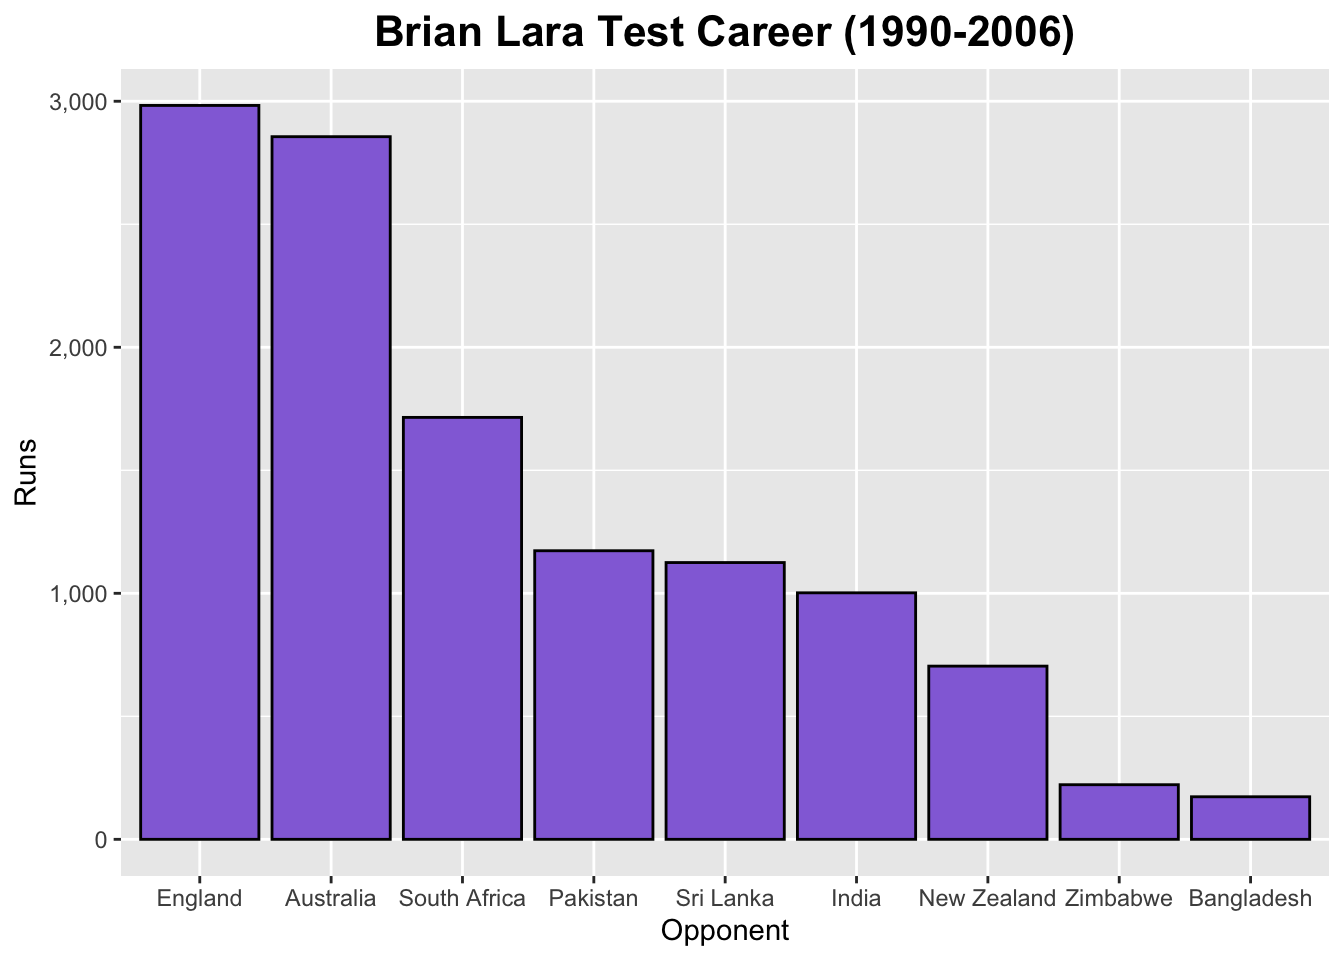
\includegraphics{gggallery_files/figure-latex/unnamed-chunk-5-1.pdf}

\hypertarget{djokovicnadal}{%
\chapter*{Djokovic vs Nadal Head-to-head}\label{djokovicnadal}}
\addcontentsline{toc}{chapter}{Djokovic vs Nadal Head-to-head}

\hypertarget{djokovicnadaldata}{%
\subsubsection*{Data}\label{djokovicnadaldata}}
\addcontentsline{toc}{subsubsection}{Data}

This plot uses the \emph{rafa\_novak} data frame from the \emph{gcubed} library. This data frame has one row for every match played between Novak Djokovic and Rafael Nadal over the course of their professional careers. In particular, the column \emph{Winner} has the name of the winner of the match.

\begin{Shaded}
\begin{Highlighting}[]
\KeywordTok{head}\NormalTok{(rafa_novak)}
\end{Highlighting}
\end{Shaded}

\begin{verbatim}
## # A tibble: 6 x 8
##    Year Event        Location   Surface   RND   Winner   Result    Loser   
##   <dbl> <chr>        <chr>      <chr>     <chr> <chr>    <chr>     <chr>   
## 1  2019 ATP Masters~ Italy      Outdoor ~ F     Rafael ~ 60 46 61  Novak D~
## 2  2019 Australian ~ Australia  Outdoor ~ F     Novak D~ 63 62 63  Rafael ~
## 3  2018 Wimbledon    Great Bri~ Outdoor ~ SF    Novak D~ 64 36 76~ Rafael ~
## 4  2018 ATP Masters~ Italy      Outdoor ~ SF    Rafael ~ 764 63    Novak D~
## 5  2017 ATP Masters~ Spain      Outdoor ~ SF    Rafael ~ 62 64     Novak D~
## 6  2016 ATP Masters~ Italy      Outdoor ~ QF    Novak D~ 75 764    Rafael ~
\end{verbatim}

This data frame is already suitable for making the plot.

\hypertarget{djokovicnadalcode}{%
\subsubsection*{Code}\label{djokovicnadalcode}}
\addcontentsline{toc}{subsubsection}{Code}

\begin{Shaded}
\begin{Highlighting}[]
\NormalTok{rafa_novak_plt <-}\StringTok{ }\KeywordTok{ggplot}\NormalTok{(rafa_novak, }\KeywordTok{aes}\NormalTok{(}\DataTypeTok{x =}\NormalTok{ Surface, }\DataTypeTok{fill =}\NormalTok{ Winner)) }\OperatorTok{+}\StringTok{ }
\StringTok{  }\KeywordTok{geom_bar}\NormalTok{(}\DataTypeTok{position =} \StringTok{"dodge"}\NormalTok{) }\OperatorTok{+}\StringTok{ }
\StringTok{  }\KeywordTok{ylab}\NormalTok{(}\StringTok{"Wins"}\NormalTok{) }\OperatorTok{+}\StringTok{ }
\StringTok{  }\KeywordTok{ggtitle}\NormalTok{(}\StringTok{"Djokovic vs Nadal Head-to-Head"}\NormalTok{) }\OperatorTok{+}\StringTok{ }
\StringTok{  }\KeywordTok{theme_bw}\NormalTok{() }\OperatorTok{+}
\StringTok{  }\KeywordTok{theme}\NormalTok{(}\DataTypeTok{panel.grid.major.x =} \KeywordTok{element_blank}\NormalTok{(),}
        \DataTypeTok{plot.title =} \KeywordTok{element_text}\NormalTok{(}\DataTypeTok{size =} \DecValTok{16}\NormalTok{, }\DataTypeTok{face =} \StringTok{"bold"}\NormalTok{, }\DataTypeTok{hjust =} \FloatTok{0.5}\NormalTok{))}

\NormalTok{rafa_novak_plt}
\end{Highlighting}
\end{Shaded}

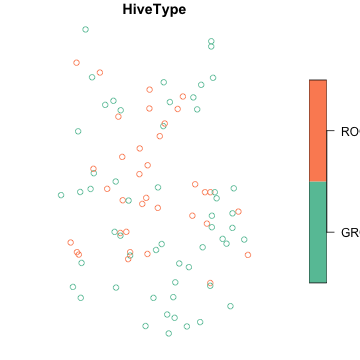
\includegraphics{gggallery_files/figure-latex/unnamed-chunk-8-1.pdf}

\hypertarget{lebron}{%
\chapter*{LeBron James Career Minutes}\label{lebron}}
\addcontentsline{toc}{chapter}{LeBron James Career Minutes}

\hypertarget{lebrondata}{%
\subsubsection*{Data}\label{lebrondata}}
\addcontentsline{toc}{subsubsection}{Data}

This plot uses the \emph{lebron\_mp} data frame from the \emph{gcubed} library. This data frame has columns \emph{MPR} and \emph{MPP} for minutes played by LeBron James during the regular season and playoffs respectively of the corresponding season.

\begin{Shaded}
\begin{Highlighting}[]
\KeywordTok{head}\NormalTok{(lebron_mp)}
\end{Highlighting}
\end{Shaded}

\begin{verbatim}
## # A tibble: 6 x 3
##   Season    MPR   MPP
##   <chr>   <dbl> <dbl>
## 1 2003-04  3122     0
## 2 2004-05  3388     0
## 3 2005-06  3361   604
## 4 2006-07  3190   893
## 5 2007-08  3027   552
## 6 2008-09  3054   580
\end{verbatim}

\hypertarget{lebroncode}{%
\subsubsection*{Code for plot}\label{lebroncode}}
\addcontentsline{toc}{subsubsection}{Code for plot}

First, add columns for cumulative career minutes for both playoffs and the regular season.

\begin{Shaded}
\begin{Highlighting}[]
\KeywordTok{library}\NormalTok{(dplyr)}

\NormalTok{df <-}\StringTok{ }\KeywordTok{mutate}\NormalTok{(lebron_mp, }\DataTypeTok{Playoffs =} \KeywordTok{cumsum}\NormalTok{(MPP),}
                    \StringTok{`}\DataTypeTok{Reg Season}\StringTok{`}\NormalTok{ =}\StringTok{ }\KeywordTok{cumsum}\NormalTok{(MPR))}
\KeywordTok{head}\NormalTok{(df)}
\end{Highlighting}
\end{Shaded}

\begin{verbatim}
## # A tibble: 6 x 5
##   Season    MPR   MPP Playoffs `Reg Season`
##   <chr>   <dbl> <dbl>    <dbl>        <dbl>
## 1 2003-04  3122     0        0         3122
## 2 2004-05  3388     0        0         6510
## 3 2005-06  3361   604      604         9871
## 4 2006-07  3190   893     1497        13061
## 5 2007-08  3027   552     2049        16088
## 6 2008-09  3054   580     2629        19142
\end{verbatim}

\begin{Shaded}
\begin{Highlighting}[]
\KeywordTok{library}\NormalTok{(tidyr)}
\NormalTok{df <-}\StringTok{ }\KeywordTok{gather}\NormalTok{(df, }\DataTypeTok{key =}\NormalTok{ RegPlayoffs, }\DataTypeTok{value =}\NormalTok{ MP, Playoffs}\OperatorTok{:}\StringTok{`}\DataTypeTok{Reg Season}\StringTok{`}\NormalTok{) }

\KeywordTok{head}\NormalTok{(df)}
\end{Highlighting}
\end{Shaded}

\begin{verbatim}
## # A tibble: 6 x 5
##   Season    MPR   MPP RegPlayoffs    MP
##   <chr>   <dbl> <dbl> <chr>       <dbl>
## 1 2003-04  3122     0 Playoffs        0
## 2 2004-05  3388     0 Playoffs        0
## 3 2005-06  3361   604 Playoffs      604
## 4 2006-07  3190   893 Playoffs     1497
## 5 2007-08  3027   552 Playoffs     2049
## 6 2008-09  3054   580 Playoffs     2629
\end{verbatim}

\begin{Shaded}
\begin{Highlighting}[]
\KeywordTok{library}\NormalTok{(ggplot2)}
\KeywordTok{library}\NormalTok{(scales)}

\NormalTok{lbj_plt <-}\StringTok{ }\KeywordTok{ggplot}\NormalTok{(df, }\KeywordTok{aes}\NormalTok{(}\DataTypeTok{x =}\NormalTok{ Season, }\DataTypeTok{y =}\NormalTok{ MP, }\DataTypeTok{fill =}\NormalTok{ RegPlayoffs)) }\OperatorTok{+}\StringTok{ }
\StringTok{  }\KeywordTok{geom_bar}\NormalTok{(}\DataTypeTok{stat =} \StringTok{"identity"}\NormalTok{) }\OperatorTok{+}\StringTok{ }
\StringTok{  }\KeywordTok{scale_fill_manual}\NormalTok{(}\DataTypeTok{values =} \KeywordTok{c}\NormalTok{(}\StringTok{"#D9717D"}\NormalTok{, }\StringTok{"#4DB6D0"}\NormalTok{)) }\OperatorTok{+}\StringTok{ }
\StringTok{  }\KeywordTok{scale_y_continuous}\NormalTok{(}\DataTypeTok{label=}\NormalTok{comma, }\DataTypeTok{limits =} \KeywordTok{c}\NormalTok{(}\DecValTok{0}\NormalTok{,}\DecValTok{70000}\NormalTok{)) }\OperatorTok{+}\StringTok{ }
\StringTok{  }\KeywordTok{theme_bw}\NormalTok{() }\OperatorTok{+}\StringTok{ }\CommentTok{#change the background colour to white}
\StringTok{  }\KeywordTok{theme}\NormalTok{(}\DataTypeTok{panel.grid.major =} \KeywordTok{element_blank}\NormalTok{(), }\DataTypeTok{panel.grid.minor =} \KeywordTok{element_blank}\NormalTok{(), }
        \DataTypeTok{axis.text.x =} \KeywordTok{element_text}\NormalTok{(}\DataTypeTok{angle =} \DecValTok{90}\NormalTok{),}
        \DataTypeTok{plot.title =} \KeywordTok{element_text}\NormalTok{(}\DataTypeTok{size =} \DecValTok{18}\NormalTok{, }\DataTypeTok{face =} \StringTok{"bold"}\NormalTok{, }\DataTypeTok{hjust =} \FloatTok{0.5}\NormalTok{),}
        \DataTypeTok{legend.title =} \KeywordTok{element_blank}\NormalTok{()}
\NormalTok{        )}\OperatorTok{+}\StringTok{ }
\StringTok{  }\KeywordTok{ylab}\NormalTok{(}\StringTok{"Cumulative Minutes"}\NormalTok{) }\OperatorTok{+}\StringTok{ }
\StringTok{  }\KeywordTok{ggtitle}\NormalTok{(}\StringTok{"LeBron James Career Minutes Played"}\NormalTok{)}

\NormalTok{lbj_plt}
\end{Highlighting}
\end{Shaded}

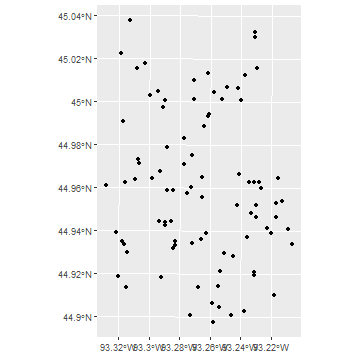
\includegraphics{gggallery_files/figure-latex/unnamed-chunk-14-1.pdf}

Adding annotations for other significant NBA players:

\begin{Shaded}
\begin{Highlighting}[]
\NormalTok{lbj_plt <-}\StringTok{ }\NormalTok{lbj_plt }\OperatorTok{+}\StringTok{ }
\StringTok{  }\KeywordTok{geom_segment}\NormalTok{(}\DataTypeTok{x =} \DecValTok{12}\NormalTok{, }\DataTypeTok{xend =} \DecValTok{17}\NormalTok{, }\DataTypeTok{y=}\DecValTok{66297}\NormalTok{, }\DataTypeTok{yend =} \DecValTok{66297}\NormalTok{, }\DataTypeTok{linetype=}\StringTok{"dashed"}\NormalTok{) }\OperatorTok{+}\StringTok{ }
\StringTok{  }\KeywordTok{geom_text}\NormalTok{(}\KeywordTok{aes}\NormalTok{(}\DecValTok{14}\NormalTok{,}\DecValTok{66297}\NormalTok{,}\DataTypeTok{label =} \StringTok{"Kareem Abdul-Jabbar"}\NormalTok{, }\DataTypeTok{vjust =} \DecValTok{-1}\NormalTok{)) }\OperatorTok{+}\StringTok{ }
\StringTok{  }\KeywordTok{geom_segment}\NormalTok{(}\DataTypeTok{x =} \DecValTok{8}\NormalTok{, }\DataTypeTok{xend =} \DecValTok{17}\NormalTok{, }\DataTypeTok{y =} \DecValTok{62759}\NormalTok{, }\DataTypeTok{yend =} \DecValTok{62759}\NormalTok{, }\DataTypeTok{linetype=}\StringTok{"dashed"}\NormalTok{) }\OperatorTok{+}\StringTok{ }
\StringTok{  }\KeywordTok{geom_text}\NormalTok{(}\KeywordTok{aes}\NormalTok{(}\DecValTok{9}\NormalTok{,}\DecValTok{62759}\NormalTok{,}\DataTypeTok{label =} \StringTok{"Karl Malone"}\NormalTok{, }\DataTypeTok{vjust =} \DecValTok{-1}\NormalTok{)) }\OperatorTok{+}
\StringTok{  }\KeywordTok{geom_segment}\NormalTok{(}\DataTypeTok{x =} \DecValTok{5}\NormalTok{, }\DataTypeTok{xend =} \DecValTok{17}\NormalTok{, }\DataTypeTok{y =} \DecValTok{57278}\NormalTok{, }\DataTypeTok{yend =} \DecValTok{57278}\NormalTok{, }\DataTypeTok{linetype=}\StringTok{"dashed"}\NormalTok{) }\OperatorTok{+}\StringTok{ }
\StringTok{  }\KeywordTok{geom_text}\NormalTok{(}\KeywordTok{aes}\NormalTok{(}\DecValTok{6}\NormalTok{,}\DecValTok{57278}\NormalTok{,}\DataTypeTok{label =} \StringTok{"Kobe Bryant"}\NormalTok{, }\DataTypeTok{vjust =} \DecValTok{-1}\NormalTok{)) }\OperatorTok{+}
\StringTok{  }\KeywordTok{geom_segment}\NormalTok{(}\DataTypeTok{x =} \DecValTok{5}\NormalTok{, }\DataTypeTok{xend =} \DecValTok{17}\NormalTok{, }\DataTypeTok{y =} \DecValTok{56738}\NormalTok{, }\DataTypeTok{yend =} \DecValTok{56738}\NormalTok{, }\DataTypeTok{linetype=}\StringTok{"dashed"}\NormalTok{) }\OperatorTok{+}\StringTok{ }
\StringTok{  }\KeywordTok{geom_text}\NormalTok{(}\KeywordTok{aes}\NormalTok{(}\DecValTok{6}\NormalTok{,}\DecValTok{56738}\NormalTok{,}\DataTypeTok{label =} \StringTok{"Tim Duncan"}\NormalTok{, }\DataTypeTok{vjust =} \FloatTok{1.5}\NormalTok{)) }\OperatorTok{+}
\StringTok{  }\KeywordTok{geom_segment}\NormalTok{(}\DataTypeTok{x =} \DecValTok{1}\NormalTok{, }\DataTypeTok{xend =} \DecValTok{17}\NormalTok{, }\DataTypeTok{y =} \DecValTok{50016}\NormalTok{, }\DataTypeTok{yend =} \DecValTok{50016}\NormalTok{, }\DataTypeTok{linetype=}\StringTok{"dashed"}\NormalTok{) }\OperatorTok{+}\StringTok{ }
\StringTok{  }\KeywordTok{geom_text}\NormalTok{(}\KeywordTok{aes}\NormalTok{(}\FloatTok{2.5}\NormalTok{,}\DecValTok{50016}\NormalTok{,}\DataTypeTok{label =} \StringTok{"Shaquille O'Neal"}\NormalTok{, }\DataTypeTok{vjust =} \DecValTok{-1}\NormalTok{)) }\OperatorTok{+}
\StringTok{  }\KeywordTok{geom_segment}\NormalTok{(}\DataTypeTok{x =} \DecValTok{1}\NormalTok{, }\DataTypeTok{xend =} \DecValTok{17}\NormalTok{, }\DataTypeTok{y =} \DecValTok{48485}\NormalTok{, }\DataTypeTok{yend =} \DecValTok{48485}\NormalTok{, }\DataTypeTok{linetype=}\StringTok{"dashed"}\NormalTok{) }\OperatorTok{+}\StringTok{ }
\StringTok{  }\KeywordTok{geom_text}\NormalTok{(}\KeywordTok{aes}\NormalTok{(}\FloatTok{2.4}\NormalTok{,}\DecValTok{48485}\NormalTok{,}\DataTypeTok{label =} \StringTok{"Michael Jordan"}\NormalTok{, }\DataTypeTok{vjust =} \FloatTok{1.5}\NormalTok{)) }\OperatorTok{+}
\StringTok{  }\KeywordTok{geom_segment}\NormalTok{(}\DataTypeTok{x =} \FloatTok{7.2}\NormalTok{, }\DataTypeTok{xend =} \DecValTok{17}\NormalTok{, }\DataTypeTok{y =} \DecValTok{41329}\NormalTok{, }\DataTypeTok{yend =} \DecValTok{41329}\NormalTok{, }\DataTypeTok{linetype=}\StringTok{"dashed"}\NormalTok{) }\OperatorTok{+}\StringTok{ }
\StringTok{  }\KeywordTok{geom_text}\NormalTok{(}\KeywordTok{aes}\NormalTok{(}\DecValTok{8}\NormalTok{,}\DecValTok{41329}\NormalTok{,}\DataTypeTok{label =} \StringTok{"Larry Bird"}\NormalTok{, }\DataTypeTok{vjust =} \DecValTok{-1}\NormalTok{)) }\OperatorTok{+}
\StringTok{  }\KeywordTok{geom_segment}\NormalTok{(}\DataTypeTok{x =} \FloatTok{7.2}\NormalTok{, }\DataTypeTok{xend =} \DecValTok{17}\NormalTok{, }\DataTypeTok{y =} \DecValTok{40783}\NormalTok{, }\DataTypeTok{yend =} \DecValTok{40783}\NormalTok{, }\DataTypeTok{linetype=}\StringTok{"dashed"}\NormalTok{) }\OperatorTok{+}
\StringTok{  }\KeywordTok{geom_text}\NormalTok{(}\KeywordTok{aes}\NormalTok{(}\FloatTok{8.5}\NormalTok{,}\DecValTok{40783}\NormalTok{,}\DataTypeTok{label =} \StringTok{"Magic Johnson"}\NormalTok{, }\DataTypeTok{vjust =} \FloatTok{1.5}\NormalTok{)) }

\NormalTok{lbj_plt}
\end{Highlighting}
\end{Shaded}

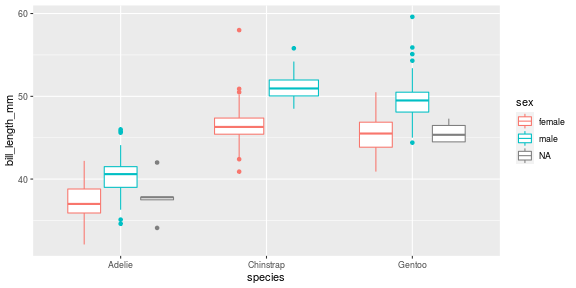
\includegraphics{gggallery_files/figure-latex/unnamed-chunk-15-1.pdf}

\hypertarget{code-for-complete-plot}{%
\paragraph{Code for complete plot}\label{code-for-complete-plot}}

\begin{Shaded}
\begin{Highlighting}[]
\NormalTok{lbj_plt <-}\StringTok{ }\KeywordTok{ggplot}\NormalTok{(df, }\KeywordTok{aes}\NormalTok{(}\DataTypeTok{x =}\NormalTok{ Season, }\DataTypeTok{y =}\NormalTok{ MP, }\DataTypeTok{fill =}\NormalTok{ RegPlayoffs)) }\OperatorTok{+}\StringTok{ }
\StringTok{  }\KeywordTok{geom_bar}\NormalTok{(}\DataTypeTok{stat =} \StringTok{"identity"}\NormalTok{) }\OperatorTok{+}\StringTok{ }
\StringTok{  }\KeywordTok{scale_fill_manual}\NormalTok{(}\DataTypeTok{values =} \KeywordTok{c}\NormalTok{(}\StringTok{"#D9717D"}\NormalTok{, }\StringTok{"#4DB6D0"}\NormalTok{)) }\OperatorTok{+}\StringTok{ }
\StringTok{  }\KeywordTok{scale_y_continuous}\NormalTok{(}\DataTypeTok{label=}\NormalTok{comma, }\DataTypeTok{limits =} \KeywordTok{c}\NormalTok{(}\DecValTok{0}\NormalTok{,}\DecValTok{70000}\NormalTok{)) }\OperatorTok{+}\StringTok{ }
\StringTok{  }\KeywordTok{theme_bw}\NormalTok{() }\OperatorTok{+}\StringTok{ }\CommentTok{#change the background colour to white}
\StringTok{  }\KeywordTok{theme}\NormalTok{(}\DataTypeTok{panel.grid.major =} \KeywordTok{element_blank}\NormalTok{(), }\DataTypeTok{panel.grid.minor =} \KeywordTok{element_blank}\NormalTok{(), }
        \DataTypeTok{axis.text.x =} \KeywordTok{element_text}\NormalTok{(}\DataTypeTok{angle =} \DecValTok{90}\NormalTok{),}
        \DataTypeTok{plot.title =} \KeywordTok{element_text}\NormalTok{(}\DataTypeTok{size =} \DecValTok{18}\NormalTok{, }\DataTypeTok{face =} \StringTok{"bold"}\NormalTok{, }\DataTypeTok{hjust =} \FloatTok{0.5}\NormalTok{),}
        \DataTypeTok{legend.title =} \KeywordTok{element_blank}\NormalTok{()}
\NormalTok{        )}\OperatorTok{+}\StringTok{ }
\StringTok{  }\KeywordTok{ylab}\NormalTok{(}\StringTok{"Cumulative Minutes"}\NormalTok{) }\OperatorTok{+}\StringTok{ }
\StringTok{  }\KeywordTok{ggtitle}\NormalTok{(}\StringTok{"LeBron James Career Minutes Played"}\NormalTok{) }\OperatorTok{+}\StringTok{ }
\StringTok{  }\KeywordTok{geom_segment}\NormalTok{(}\DataTypeTok{x =} \DecValTok{12}\NormalTok{, }\DataTypeTok{xend =} \DecValTok{17}\NormalTok{, }\DataTypeTok{y=}\DecValTok{66297}\NormalTok{, }\DataTypeTok{yend =} \DecValTok{66297}\NormalTok{, }\DataTypeTok{linetype=}\StringTok{"dashed"}\NormalTok{) }\OperatorTok{+}\StringTok{ }
\StringTok{  }\KeywordTok{geom_text}\NormalTok{(}\KeywordTok{aes}\NormalTok{(}\DecValTok{14}\NormalTok{,}\DecValTok{66297}\NormalTok{,}\DataTypeTok{label =} \StringTok{"Kareem Abdul-Jabbar"}\NormalTok{, }\DataTypeTok{vjust =} \DecValTok{-1}\NormalTok{)) }\OperatorTok{+}\StringTok{ }
\StringTok{  }\KeywordTok{geom_segment}\NormalTok{(}\DataTypeTok{x =} \DecValTok{8}\NormalTok{, }\DataTypeTok{xend =} \DecValTok{17}\NormalTok{, }\DataTypeTok{y =} \DecValTok{62759}\NormalTok{, }\DataTypeTok{yend =} \DecValTok{62759}\NormalTok{, }\DataTypeTok{linetype=}\StringTok{"dashed"}\NormalTok{) }\OperatorTok{+}\StringTok{ }
\StringTok{  }\KeywordTok{geom_text}\NormalTok{(}\KeywordTok{aes}\NormalTok{(}\DecValTok{9}\NormalTok{,}\DecValTok{62759}\NormalTok{,}\DataTypeTok{label =} \StringTok{"Karl Malone"}\NormalTok{, }\DataTypeTok{vjust =} \DecValTok{-1}\NormalTok{)) }\OperatorTok{+}
\StringTok{  }\KeywordTok{geom_segment}\NormalTok{(}\DataTypeTok{x =} \DecValTok{5}\NormalTok{, }\DataTypeTok{xend =} \DecValTok{17}\NormalTok{, }\DataTypeTok{y =} \DecValTok{57278}\NormalTok{, }\DataTypeTok{yend =} \DecValTok{57278}\NormalTok{, }\DataTypeTok{linetype=}\StringTok{"dashed"}\NormalTok{) }\OperatorTok{+}\StringTok{ }
\StringTok{  }\KeywordTok{geom_text}\NormalTok{(}\KeywordTok{aes}\NormalTok{(}\DecValTok{6}\NormalTok{,}\DecValTok{57278}\NormalTok{,}\DataTypeTok{label =} \StringTok{"Kobe Bryant"}\NormalTok{, }\DataTypeTok{vjust =} \DecValTok{-1}\NormalTok{)) }\OperatorTok{+}
\StringTok{  }\KeywordTok{geom_segment}\NormalTok{(}\DataTypeTok{x =} \DecValTok{5}\NormalTok{, }\DataTypeTok{xend =} \DecValTok{17}\NormalTok{, }\DataTypeTok{y =} \DecValTok{56738}\NormalTok{, }\DataTypeTok{yend =} \DecValTok{56738}\NormalTok{, }\DataTypeTok{linetype=}\StringTok{"dashed"}\NormalTok{) }\OperatorTok{+}\StringTok{ }
\StringTok{  }\KeywordTok{geom_text}\NormalTok{(}\KeywordTok{aes}\NormalTok{(}\DecValTok{6}\NormalTok{,}\DecValTok{56738}\NormalTok{,}\DataTypeTok{label =} \StringTok{"Tim Duncan"}\NormalTok{, }\DataTypeTok{vjust =} \FloatTok{1.5}\NormalTok{)) }\OperatorTok{+}
\StringTok{  }\KeywordTok{geom_segment}\NormalTok{(}\DataTypeTok{x =} \DecValTok{1}\NormalTok{, }\DataTypeTok{xend =} \DecValTok{17}\NormalTok{, }\DataTypeTok{y =} \DecValTok{50016}\NormalTok{, }\DataTypeTok{yend =} \DecValTok{50016}\NormalTok{, }\DataTypeTok{linetype=}\StringTok{"dashed"}\NormalTok{) }\OperatorTok{+}\StringTok{ }
\StringTok{  }\KeywordTok{geom_text}\NormalTok{(}\KeywordTok{aes}\NormalTok{(}\FloatTok{2.5}\NormalTok{,}\DecValTok{50016}\NormalTok{,}\DataTypeTok{label =} \StringTok{"Shaquille O'Neal"}\NormalTok{, }\DataTypeTok{vjust =} \DecValTok{-1}\NormalTok{)) }\OperatorTok{+}
\StringTok{  }\KeywordTok{geom_segment}\NormalTok{(}\DataTypeTok{x =} \DecValTok{1}\NormalTok{, }\DataTypeTok{xend =} \DecValTok{17}\NormalTok{, }\DataTypeTok{y =} \DecValTok{48485}\NormalTok{, }\DataTypeTok{yend =} \DecValTok{48485}\NormalTok{, }\DataTypeTok{linetype=}\StringTok{"dashed"}\NormalTok{) }\OperatorTok{+}\StringTok{ }
\StringTok{  }\KeywordTok{geom_text}\NormalTok{(}\KeywordTok{aes}\NormalTok{(}\FloatTok{2.4}\NormalTok{,}\DecValTok{48485}\NormalTok{,}\DataTypeTok{label =} \StringTok{"Michael Jordan"}\NormalTok{, }\DataTypeTok{vjust =} \FloatTok{1.5}\NormalTok{)) }\OperatorTok{+}
\StringTok{  }\KeywordTok{geom_segment}\NormalTok{(}\DataTypeTok{x =} \FloatTok{7.2}\NormalTok{, }\DataTypeTok{xend =} \DecValTok{17}\NormalTok{, }\DataTypeTok{y =} \DecValTok{41329}\NormalTok{, }\DataTypeTok{yend =} \DecValTok{41329}\NormalTok{, }\DataTypeTok{linetype=}\StringTok{"dashed"}\NormalTok{) }\OperatorTok{+}\StringTok{ }
\StringTok{  }\KeywordTok{geom_text}\NormalTok{(}\KeywordTok{aes}\NormalTok{(}\DecValTok{8}\NormalTok{,}\DecValTok{41329}\NormalTok{,}\DataTypeTok{label =} \StringTok{"Larry Bird"}\NormalTok{, }\DataTypeTok{vjust =} \DecValTok{-1}\NormalTok{)) }\OperatorTok{+}
\StringTok{  }\KeywordTok{geom_segment}\NormalTok{(}\DataTypeTok{x =} \FloatTok{7.2}\NormalTok{, }\DataTypeTok{xend =} \DecValTok{17}\NormalTok{, }\DataTypeTok{y =} \DecValTok{40783}\NormalTok{, }\DataTypeTok{yend =} \DecValTok{40783}\NormalTok{, }\DataTypeTok{linetype=}\StringTok{"dashed"}\NormalTok{) }\OperatorTok{+}
\StringTok{  }\KeywordTok{geom_text}\NormalTok{(}\KeywordTok{aes}\NormalTok{(}\FloatTok{8.5}\NormalTok{,}\DecValTok{40783}\NormalTok{,}\DataTypeTok{label =} \StringTok{"Magic Johnson"}\NormalTok{, }\DataTypeTok{vjust =} \FloatTok{1.5}\NormalTok{)) }
\end{Highlighting}
\end{Shaded}

\hypertarget{energy18}{%
\chapter*{Global Energy Consumption 2018}\label{energy18}}
\addcontentsline{toc}{chapter}{Global Energy Consumption 2018}

\hypertarget{energy18data}{%
\subsubsection*{Data}\label{energy18data}}
\addcontentsline{toc}{subsubsection}{Data}

This plot uses the \emph{energy18} data frame of the \emph{gcubed} package.

\begin{Shaded}
\begin{Highlighting}[]
\KeywordTok{head}\NormalTok{(energy18)}
\end{Highlighting}
\end{Shaded}

\begin{verbatim}
## # A tibble: 6 x 8
##   Countries   Oil `Natural Gas`  Coal Nuclear Hydroelectric Renewable
##   <chr>     <dbl>         <dbl> <dbl>   <dbl>         <dbl>     <dbl>
## 1 Canada    110            99.5  14.4    22.6          87.6      10.3
## 2 Mexico     82.8          77    11.9     3.1           7.3       4.8
## 3 US        920.          703.  317     192.           65.3     104. 
## 4 Argentina  30.1          41.9   1.2     1.6           9.4       0.9
## 5 Brazil    136.           30.9  15.9     3.5          87.7      23.6
## 6 Chile      18.1           5.5   7.7     0             5.2       3.5
## # ... with 1 more variable: Region <chr>
\end{verbatim}

First get totals for each energy source (natural gas, oil, coal, nuclear, hydroelectric, renewable) for each region:

\begin{Shaded}
\begin{Highlighting}[]
\KeywordTok{library}\NormalTok{(dplyr)}

\NormalTok{df <-}\StringTok{ }\KeywordTok{group_by}\NormalTok{(energy18, Region) }\OperatorTok\StringTok{ }
\StringTok{  }\KeywordTok{summarise}\NormalTok{(}\DataTypeTok{Oil =} \KeywordTok{sum}\NormalTok{(Oil),}
            \StringTok{`}\DataTypeTok{Natural Gas}\StringTok{`}\NormalTok{ =}\StringTok{ }\KeywordTok{sum}\NormalTok{(}\StringTok{`}\DataTypeTok{Natural Gas}\StringTok{`}\NormalTok{),}
            \DataTypeTok{Coal =} \KeywordTok{sum}\NormalTok{(Coal),}
            \DataTypeTok{Nuclear =} \KeywordTok{sum}\NormalTok{(Nuclear), }
            \DataTypeTok{Hydroelectric =} \KeywordTok{sum}\NormalTok{(Hydroelectric), }
            \DataTypeTok{Renewable =} \KeywordTok{sum}\NormalTok{(Renewable))}
\KeywordTok{head}\NormalTok{(df)}
\end{Highlighting}
\end{Shaded}

\begin{verbatim}
## # A tibble: 6 x 7
##   Region          Oil `Natural Gas`   Coal Nuclear Hydroelectric Renewable
##   <chr>         <dbl>         <dbl>  <dbl>   <dbl>         <dbl>     <dbl>
## 1 Africa         191.          129.  101.      2.5          30.1       7.2
## 2 Asia Pacific  1695.          710. 2841.    125.          389.      225. 
## 3 CIS            194.          499.  135.     46.8          55.4       0.5
## 4 Europe         742.          472.  307.    212.          145.      172. 
## 5 Middle East    412           475.    8.1     1.6           3.4       1.6
## 6 North America 1112.          879.  343.    218.          160.      119.
\end{verbatim}

Now use the \textbf{gather} command of the \textbf{tidyr} package to get all the energy values into the same column while creating an accompanying column to indicate the energy source.

\begin{Shaded}
\begin{Highlighting}[]
\KeywordTok{library}\NormalTok{(tidyr)}
\NormalTok{df <-}\StringTok{ }\KeywordTok{gather}\NormalTok{(df, }\DataTypeTok{key =}\NormalTok{ Type, }\DataTypeTok{value =}\NormalTok{ Energy, }\DecValTok{-1}\NormalTok{)}

\KeywordTok{head}\NormalTok{(df)}
\end{Highlighting}
\end{Shaded}

\begin{verbatim}
## # A tibble: 6 x 3
##   Region        Type  Energy
##   <chr>         <chr>  <dbl>
## 1 Africa        Oil     191.
## 2 Asia Pacific  Oil    1695.
## 3 CIS           Oil     194.
## 4 Europe        Oil     742.
## 5 Middle East   Oil     412 
## 6 North America Oil    1112.
\end{verbatim}

The \emph{df} data frame is now suitable for making the plot.

\hypertarget{energy18code}{%
\subsubsection*{Code}\label{energy18code}}
\addcontentsline{toc}{subsubsection}{Code}

\begin{Shaded}
\begin{Highlighting}[]
\KeywordTok{library}\NormalTok{(ggplot2)}
\KeywordTok{library}\NormalTok{(scales) }\CommentTok{#for formatting the axes labels to have commas e.g. 1,000 }

\NormalTok{df}\OperatorTok{$}\NormalTok{Type <-}\StringTok{ }\KeywordTok{factor}\NormalTok{(df}\OperatorTok{$}\NormalTok{Type)}
\NormalTok{energy_plt <-}\StringTok{ }\KeywordTok{ggplot}\NormalTok{(df, }\KeywordTok{aes}\NormalTok{(Type, Energy, }\DataTypeTok{fill =}\NormalTok{ Type)) }\OperatorTok{+}\StringTok{ }\KeywordTok{geom_bar}\NormalTok{(}\DataTypeTok{stat =} \StringTok{"identity"}\NormalTok{) }\OperatorTok{+}\StringTok{ }
\StringTok{  }\KeywordTok{facet_wrap}\NormalTok{(}\OperatorTok{~}\NormalTok{Region, }\DataTypeTok{ncol =} \DecValTok{2}\NormalTok{, }\DataTypeTok{scale =} \StringTok{"free"}\NormalTok{) }\OperatorTok{+}\StringTok{ }\KeywordTok{coord_flip}\NormalTok{() }\OperatorTok{+}\StringTok{ }
\StringTok{  }\KeywordTok{scale_x_discrete}\NormalTok{(}\DataTypeTok{limits =} \KeywordTok{rev}\NormalTok{(}\KeywordTok{levels}\NormalTok{(df}\OperatorTok{$}\NormalTok{Type))) }\OperatorTok{+}\StringTok{ }
\StringTok{  }\KeywordTok{scale_y_continuous}\NormalTok{(}\DataTypeTok{label =}\NormalTok{ comma) }\OperatorTok{+}\StringTok{ }
\StringTok{  }\KeywordTok{xlab}\NormalTok{(}\StringTok{""}\NormalTok{) }\OperatorTok{+}\StringTok{ }
\StringTok{  }\KeywordTok{ylab}\NormalTok{(}\StringTok{"Million tonnes oil equivalent"}\NormalTok{) }\OperatorTok{+}
\StringTok{  }\KeywordTok{theme}\NormalTok{(}\DataTypeTok{plot.title =} \KeywordTok{element_text}\NormalTok{(}\DataTypeTok{size =} \DecValTok{16}\NormalTok{, }\DataTypeTok{face =} \StringTok{"bold"}\NormalTok{, }\DataTypeTok{hjust =} \FloatTok{0.5}\NormalTok{),}
        \DataTypeTok{legend.title =} \KeywordTok{element_blank}\NormalTok{()) }\OperatorTok{+}\StringTok{ }
\StringTok{  }\KeywordTok{ggtitle}\NormalTok{(}\StringTok{"Global Energy Consumption (2018)"}\NormalTok{)  }

\NormalTok{energy_plt}
\end{Highlighting}
\end{Shaded}

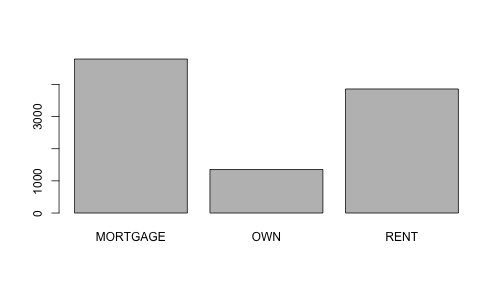
\includegraphics{gggallery_files/figure-latex/unnamed-chunk-22-1.pdf}

\hypertarget{iris}{%
\chapter*{Iris Data Set}\label{iris}}
\addcontentsline{toc}{chapter}{Iris Data Set}

\hypertarget{irisdata}{%
\subsubsection*{Data}\label{irisdata}}
\addcontentsline{toc}{subsubsection}{Data}

This plot uses the \emph{iris} data set that comes with R. This data frame contains the widths and lengths of the petals and sepals of 150 iris flowers.
The flowers are of three different species: setosa, versicolor and virginica. There are 50 specimens of each species.

\begin{Shaded}
\begin{Highlighting}[]
\KeywordTok{head}\NormalTok{(iris)}
\end{Highlighting}
\end{Shaded}

\begin{verbatim}
##   Sepal.Length Sepal.Width Petal.Length Petal.Width Species
## 1          5.1         3.5          1.4         0.2  setosa
## 2          4.9         3.0          1.4         0.2  setosa
## 3          4.7         3.2          1.3         0.2  setosa
## 4          4.6         3.1          1.5         0.2  setosa
## 5          5.0         3.6          1.4         0.2  setosa
## 6          5.4         3.9          1.7         0.4  setosa
\end{verbatim}

\hypertarget{iriscode}{%
\subsubsection*{Code for plot}\label{iriscode}}
\addcontentsline{toc}{subsubsection}{Code for plot}

\begin{Shaded}
\begin{Highlighting}[]
\NormalTok{iris_petal_plot <-}\StringTok{ }\KeywordTok{ggplot}\NormalTok{(}\DataTypeTok{data =}\NormalTok{ iris, }\KeywordTok{aes}\NormalTok{(}\DataTypeTok{x =}\NormalTok{ Petal.Width, }\DataTypeTok{y =}\NormalTok{ Petal.Length, }\DataTypeTok{colour =}\NormalTok{ Species)) }\OperatorTok{+}\StringTok{ }
\StringTok{  }\KeywordTok{geom_point}\NormalTok{() }\OperatorTok{+}\StringTok{ }\KeywordTok{theme_bw}\NormalTok{() }\OperatorTok{+}
\StringTok{  }\KeywordTok{xlab}\NormalTok{(}\StringTok{"Petal Width (cm)"}\NormalTok{) }\OperatorTok{+}\StringTok{ }
\StringTok{  }\KeywordTok{ylab}\NormalTok{(}\StringTok{"Petal Length (cm)"}\NormalTok{) }\OperatorTok{+}\StringTok{ }
\StringTok{  }\KeywordTok{ggtitle}\NormalTok{(}\StringTok{"Petals of the iris data set"}\NormalTok{) }\OperatorTok{+}\StringTok{ }
\StringTok{  }\KeywordTok{theme}\NormalTok{(}\DataTypeTok{plot.title =} \KeywordTok{element_text}\NormalTok{(}\DataTypeTok{size =} \DecValTok{16}\NormalTok{, }\DataTypeTok{face =} \StringTok{"bold"}\NormalTok{, }\DataTypeTok{hjust =} \FloatTok{0.5}\NormalTok{))}

\NormalTok{iris_petal_plot}
\end{Highlighting}
\end{Shaded}

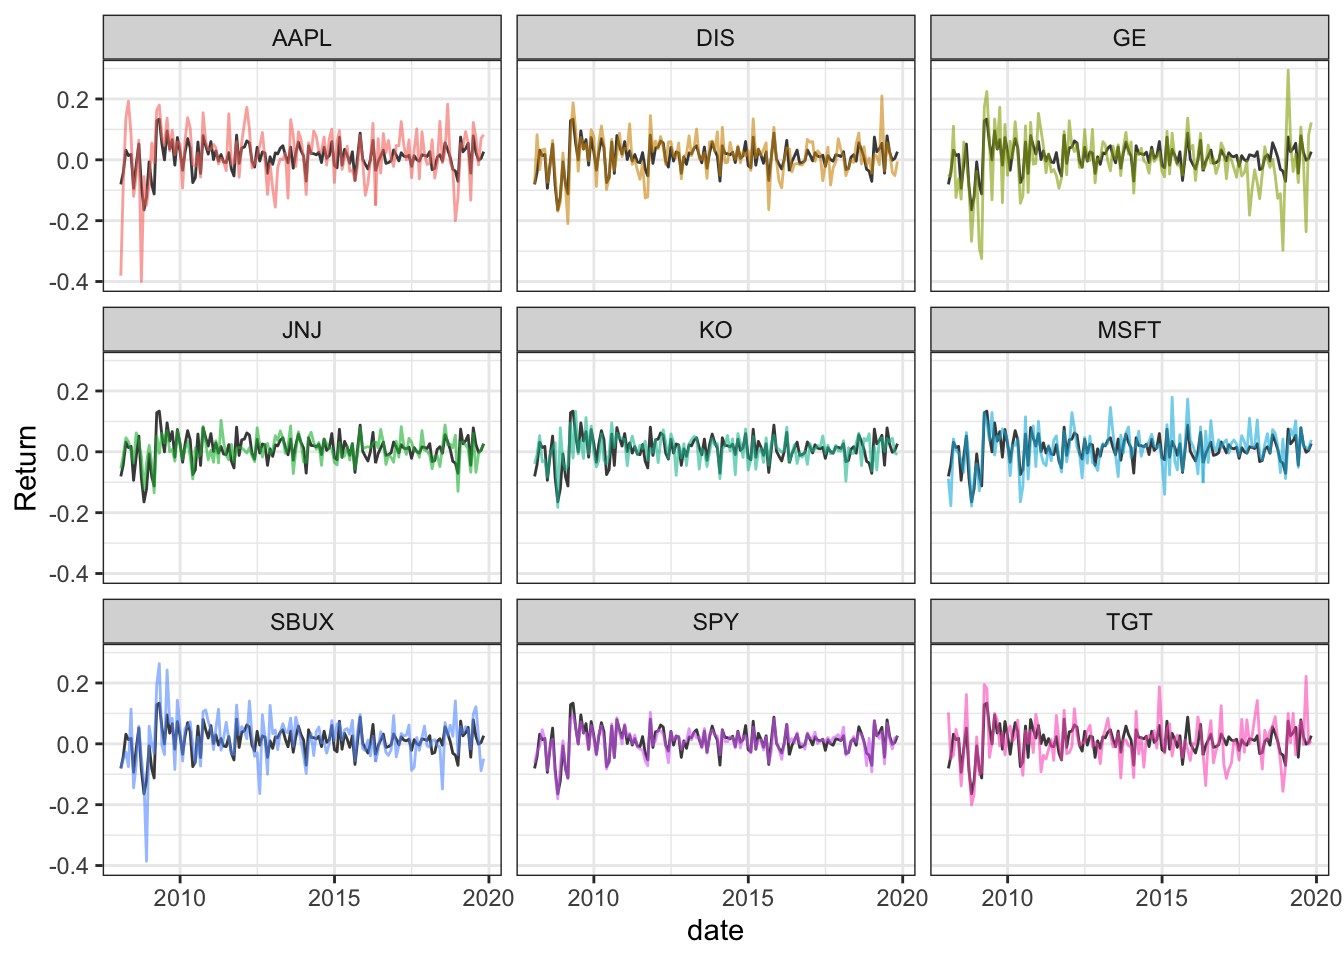
\includegraphics{gggallery_files/figure-latex/unnamed-chunk-25-1.pdf}

\hypertarget{unemp}{%
\chapter*{10 Yr History of US Unemployment: Line Chart}\label{unemp}}
\addcontentsline{toc}{chapter}{10 Yr History of US Unemployment: Line Chart}

\hypertarget{unempdata}{%
\subsubsection*{Data}\label{unempdata}}
\addcontentsline{toc}{subsubsection}{Data}

This plot uses the \emph{us\_unemp} data frame of the \emph{gcubed} package. This data frame contains \href{https://data.bls.gov/timeseries/LNS14000000}{unemployment rates for the United States} published by the Bureau of Labor and Statistics. Rates are published monthly.

\begin{Shaded}
\begin{Highlighting}[]
\KeywordTok{head}\NormalTok{(us_unemp)}
\end{Highlighting}
\end{Shaded}

\begin{verbatim}
## # A tibble: 6 x 2
##   Date        Rate
##   <date>     <dbl>
## 1 2010-01-01   9.8
## 2 2010-02-01   9.8
## 3 2010-03-01   9.9
## 4 2010-04-01   9.9
## 5 2010-05-01   9.6
## 6 2010-06-01   9.4
\end{verbatim}

\hypertarget{unempcode}{%
\subsubsection*{Code for plot}\label{unempcode}}
\addcontentsline{toc}{subsubsection}{Code for plot}

This plot uses \emph{geom\_line} to create a line chart.

\begin{Shaded}
\begin{Highlighting}[]
\NormalTok{unemp_plt <-}\StringTok{ }\KeywordTok{ggplot}\NormalTok{(us_unemp, }\KeywordTok{aes}\NormalTok{(}\DataTypeTok{x =}\NormalTok{ Date, }\DataTypeTok{y =}\NormalTok{ Rate)) }\OperatorTok{+}\StringTok{ }
\StringTok{  }\KeywordTok{geom_line}\NormalTok{() }\OperatorTok{+}\StringTok{ }
\StringTok{  }\KeywordTok{ggtitle}\NormalTok{(}\StringTok{"10 Year History of US Unemployment Rates (2004 - 2019)"}\NormalTok{)}

\NormalTok{unemp_plt}
\end{Highlighting}
\end{Shaded}

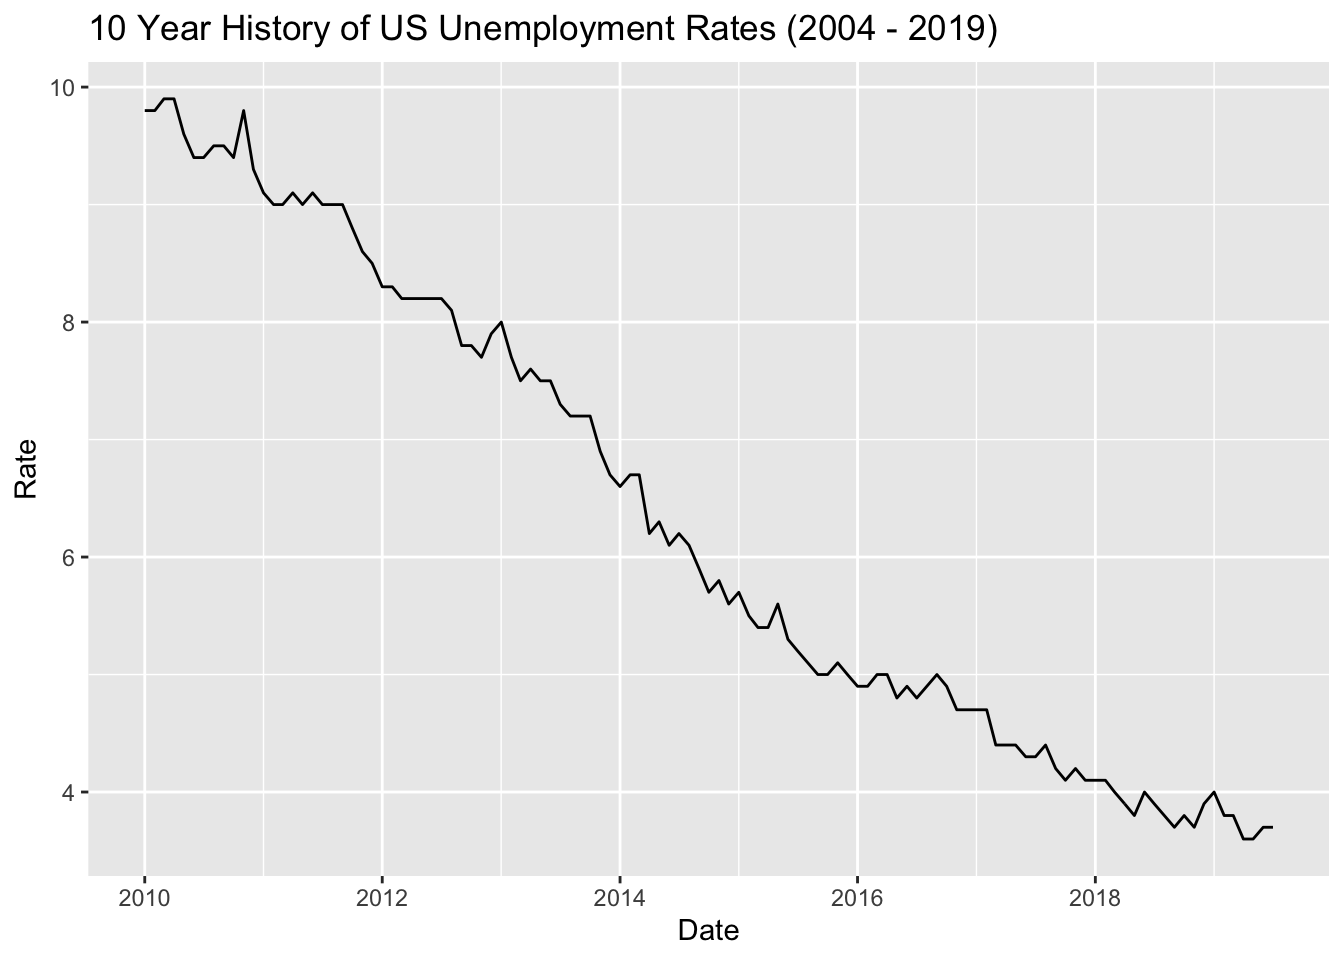
\includegraphics{gggallery_files/figure-latex/unnamed-chunk-29-1.pdf}

\hypertarget{unempp}{%
\chapter*{10 Yr History of US Unemployment: Line and Point plot}\label{unempp}}
\addcontentsline{toc}{chapter}{10 Yr History of US Unemployment: Line and Point plot}

\hypertarget{unemppdata}{%
\subsubsection*{Data}\label{unemppdata}}
\addcontentsline{toc}{subsubsection}{Data}

This plot uses the \emph{us\_unemp} data frame of the \emph{gcubed} package. This data frame contains \href{https://data.bls.gov/timeseries/LNS14000000}{unemployment rates for the United States} published by the Bureau of Labor and Statistics. Rates are published monthly.

\begin{Shaded}
\begin{Highlighting}[]
\KeywordTok{head}\NormalTok{(us_unemp)}
\end{Highlighting}
\end{Shaded}

\begin{verbatim}
## # A tibble: 6 x 2
##   Date        Rate
##   <date>     <dbl>
## 1 2010-01-01   9.8
## 2 2010-02-01   9.8
## 3 2010-03-01   9.9
## 4 2010-04-01   9.9
## 5 2010-05-01   9.6
## 6 2010-06-01   9.4
\end{verbatim}

\hypertarget{unemppcode}{%
\subsubsection*{Code for plot}\label{unemppcode}}
\addcontentsline{toc}{subsubsection}{Code for plot}

This plot uses \emph{geom\_line} (to create the line chart) and \emph{geom\_point} to highlight the data
points simultaneously.

\begin{Shaded}
\begin{Highlighting}[]
\NormalTok{unemp_ptline_plt <-}\StringTok{ }\KeywordTok{ggplot}\NormalTok{(us_unemp, }\KeywordTok{aes}\NormalTok{(}\DataTypeTok{x =}\NormalTok{ Date, }\DataTypeTok{y =}\NormalTok{ Rate)) }\OperatorTok{+}\StringTok{ }
\StringTok{  }\KeywordTok{geom_line}\NormalTok{() }\OperatorTok{+}\StringTok{ }\KeywordTok{geom_point}\NormalTok{() }\OperatorTok{+}
\StringTok{  }\KeywordTok{ggtitle}\NormalTok{(}\StringTok{"10 Year History of US Unemployment Rates (2004 - 2019)"}\NormalTok{)  }\OperatorTok{+}
\StringTok{  }\KeywordTok{theme_bw}\NormalTok{()}

\NormalTok{unemp_ptline_plt}
\end{Highlighting}
\end{Shaded}

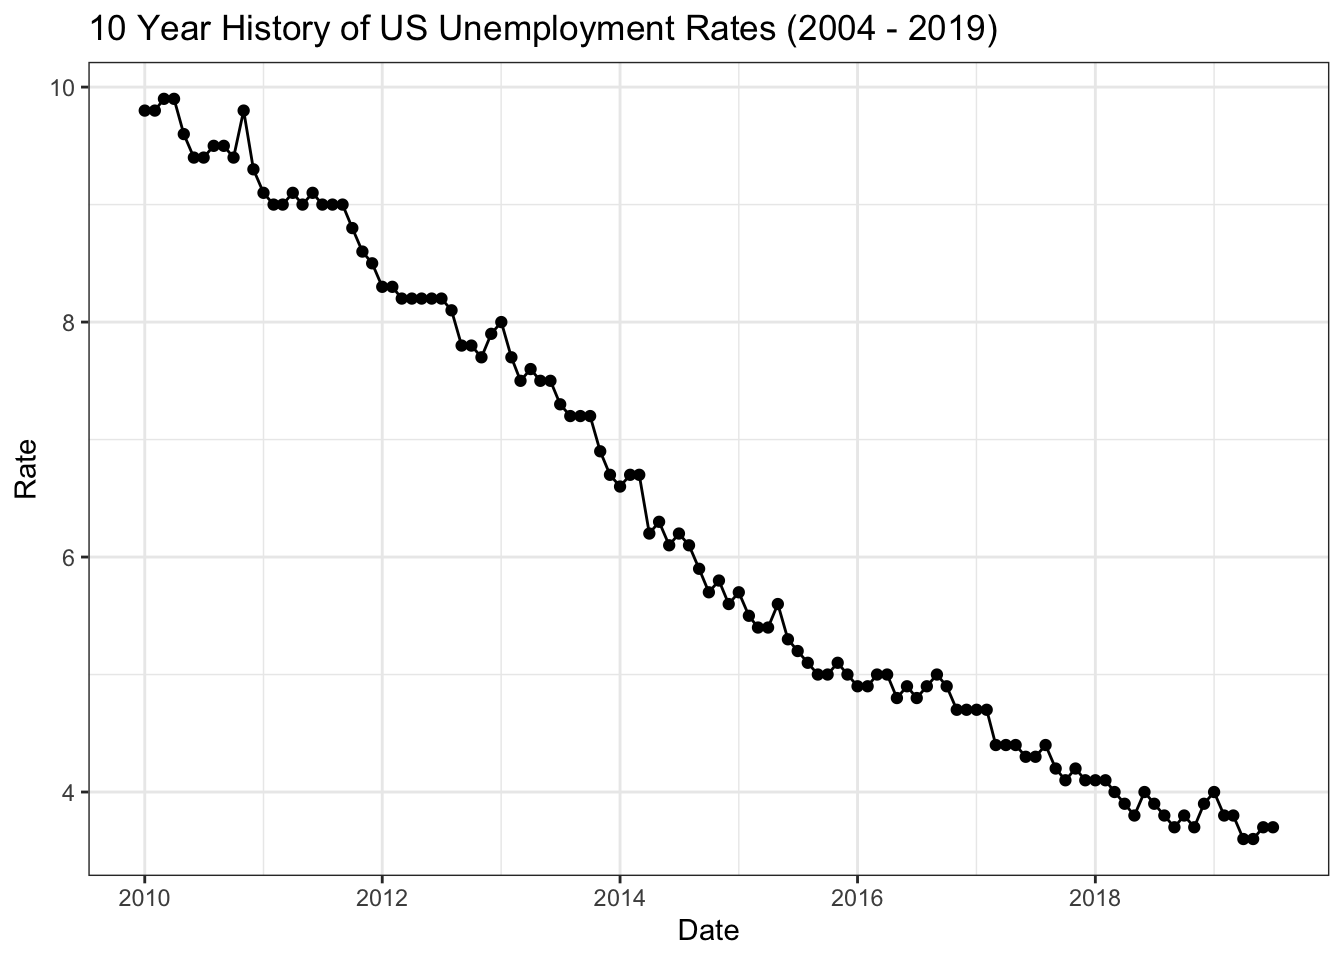
\includegraphics{gggallery_files/figure-latex/unnamed-chunk-32-1.pdf}

\hypertarget{unemppp}{%
\chapter*{10 Yr History of US Unemployment: Lollipop chart}\label{unemppp}}
\addcontentsline{toc}{chapter}{10 Yr History of US Unemployment: Lollipop chart}

\hypertarget{unempppdata}{%
\subsubsection*{Data}\label{unempppdata}}
\addcontentsline{toc}{subsubsection}{Data}

This plot uses the \emph{us\_unemp} data frame of the \emph{gcubed} package. This data frame contains \href{https://data.bls.gov/timeseries/LNS14000000}{unemployment rates for the United States} published by the Bureau of Labor and Statistics. Rates are published monthly.

\begin{Shaded}
\begin{Highlighting}[]
\KeywordTok{head}\NormalTok{(us_unemp)}
\end{Highlighting}
\end{Shaded}

\begin{verbatim}
## # A tibble: 6 x 2
##   Date        Rate
##   <date>     <dbl>
## 1 2010-01-01   9.8
## 2 2010-02-01   9.8
## 3 2010-03-01   9.9
## 4 2010-04-01   9.9
## 5 2010-05-01   9.6
## 6 2010-06-01   9.4
\end{verbatim}

\hypertarget{unempppcode}{%
\subsubsection*{Code for plot}\label{unempppcode}}
\addcontentsline{toc}{subsubsection}{Code for plot}

\begin{Shaded}
\begin{Highlighting}[]
\NormalTok{unemp_plt <-}\StringTok{ }\KeywordTok{ggplot}\NormalTok{(us_unemp, }\KeywordTok{aes}\NormalTok{(}\DataTypeTok{x =}\NormalTok{ Date, }\DataTypeTok{y =}\NormalTok{ Rate)) }\OperatorTok{+}\StringTok{ }\KeywordTok{geom_point}\NormalTok{() }\OperatorTok{+}\StringTok{ }
\StringTok{  }\KeywordTok{geom_segment}\NormalTok{(}\KeywordTok{aes}\NormalTok{(}\DataTypeTok{x =}\NormalTok{ Date, }\DataTypeTok{xend =}\NormalTok{ Date, }\DataTypeTok{y =} \DecValTok{0}\NormalTok{, }\DataTypeTok{yend =}\NormalTok{ Rate)) }\OperatorTok{+}\StringTok{ }
\StringTok{  }\KeywordTok{ggtitle}\NormalTok{(}\StringTok{"10 Year History of US Unemployment Rates (2004 - 2019)"}\NormalTok{)  }\OperatorTok{+}
\StringTok{  }\KeywordTok{theme_bw}\NormalTok{()}


\NormalTok{unemp_plt}
\end{Highlighting}
\end{Shaded}

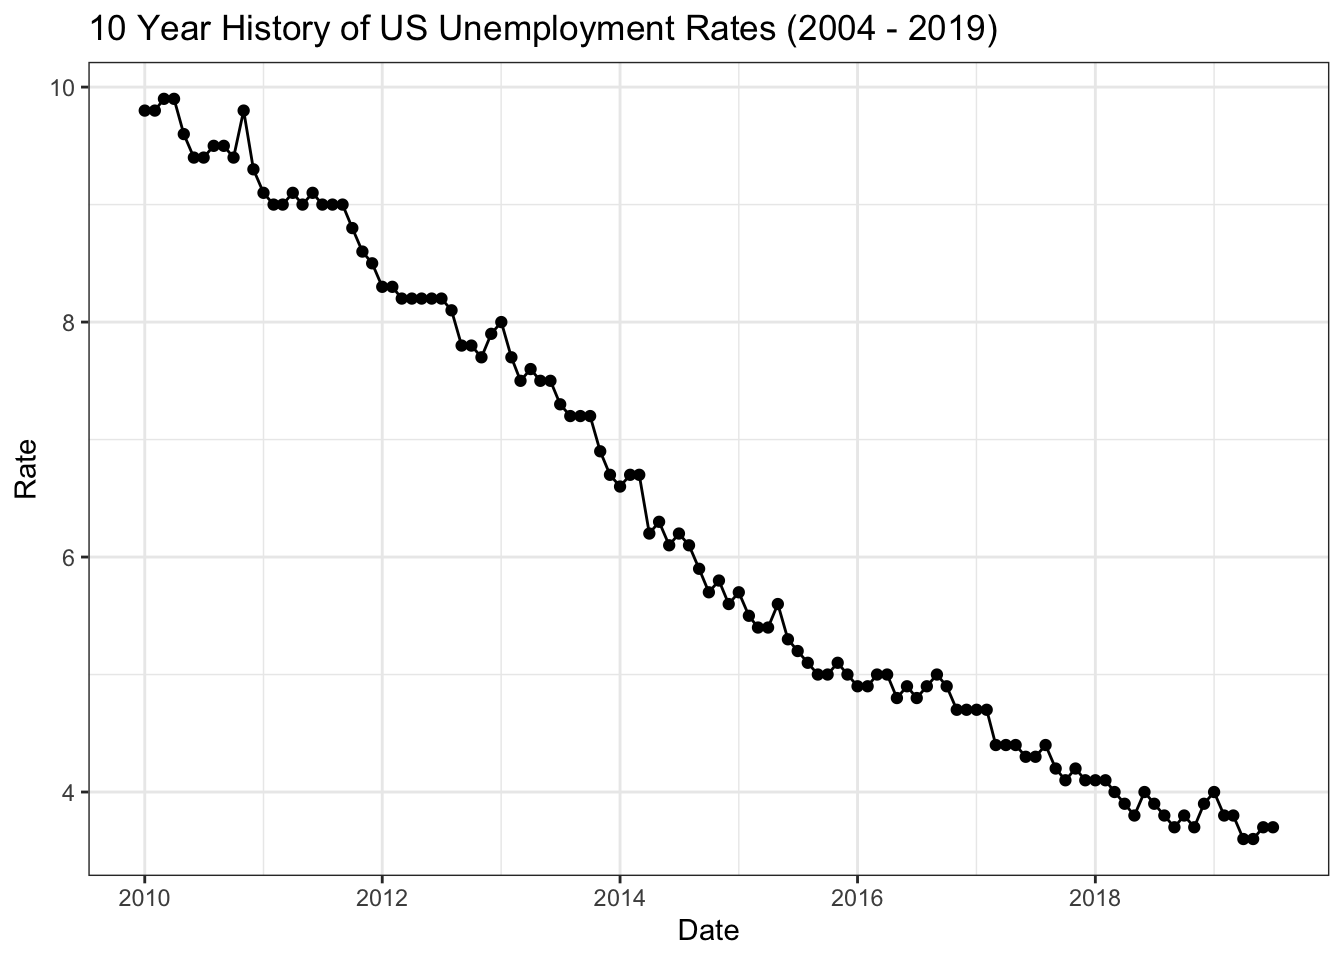
\includegraphics{gggallery_files/figure-latex/unnamed-chunk-35-1.pdf}

\hypertarget{unempppp}{%
\chapter*{10 Yr History of US Unemployment: Step Plot}\label{unempppp}}
\addcontentsline{toc}{chapter}{10 Yr History of US Unemployment: Step Plot}

\hypertarget{unemppppdata}{%
\subsubsection*{Data}\label{unemppppdata}}
\addcontentsline{toc}{subsubsection}{Data}

This plot uses the \emph{us\_unemp} data frame of the \emph{gcubed} package. This data frame contains \href{https://data.bls.gov/timeseries/LNS14000000}{unemployment rates for the United States} published by the Bureau of Labor and Statistics. Rates are published monthly.

\begin{Shaded}
\begin{Highlighting}[]
\KeywordTok{head}\NormalTok{(us_unemp)}
\end{Highlighting}
\end{Shaded}

\begin{verbatim}
## # A tibble: 6 x 2
##   Date        Rate
##   <date>     <dbl>
## 1 2010-01-01   9.8
## 2 2010-02-01   9.8
## 3 2010-03-01   9.9
## 4 2010-04-01   9.9
## 5 2010-05-01   9.6
## 6 2010-06-01   9.4
\end{verbatim}

\hypertarget{unemppppcode}{%
\subsubsection*{Code for plot}\label{unemppppcode}}
\addcontentsline{toc}{subsubsection}{Code for plot}

This plot uses the \emph{geom\_step} geometry to get a step function appearance as opposed to the look of using \protect\hyperlink{unemp1code}{\emph{geom\_line}}.

\begin{Shaded}
\begin{Highlighting}[]
\NormalTok{unemp_step_plt <-}\StringTok{ }\KeywordTok{ggplot}\NormalTok{(us_unemp, }\KeywordTok{aes}\NormalTok{(}\DataTypeTok{x =}\NormalTok{ Date, }\DataTypeTok{y =}\NormalTok{ Rate)) }\OperatorTok{+}\StringTok{ }\KeywordTok{geom_step}\NormalTok{() }\OperatorTok{+}\StringTok{ }
\StringTok{  }\KeywordTok{ggtitle}\NormalTok{(}\StringTok{"10 Year History of US Unemployment Rates (2004 - 2019)"}\NormalTok{)}
  
  
\NormalTok{unemp_step_plt}
\end{Highlighting}
\end{Shaded}

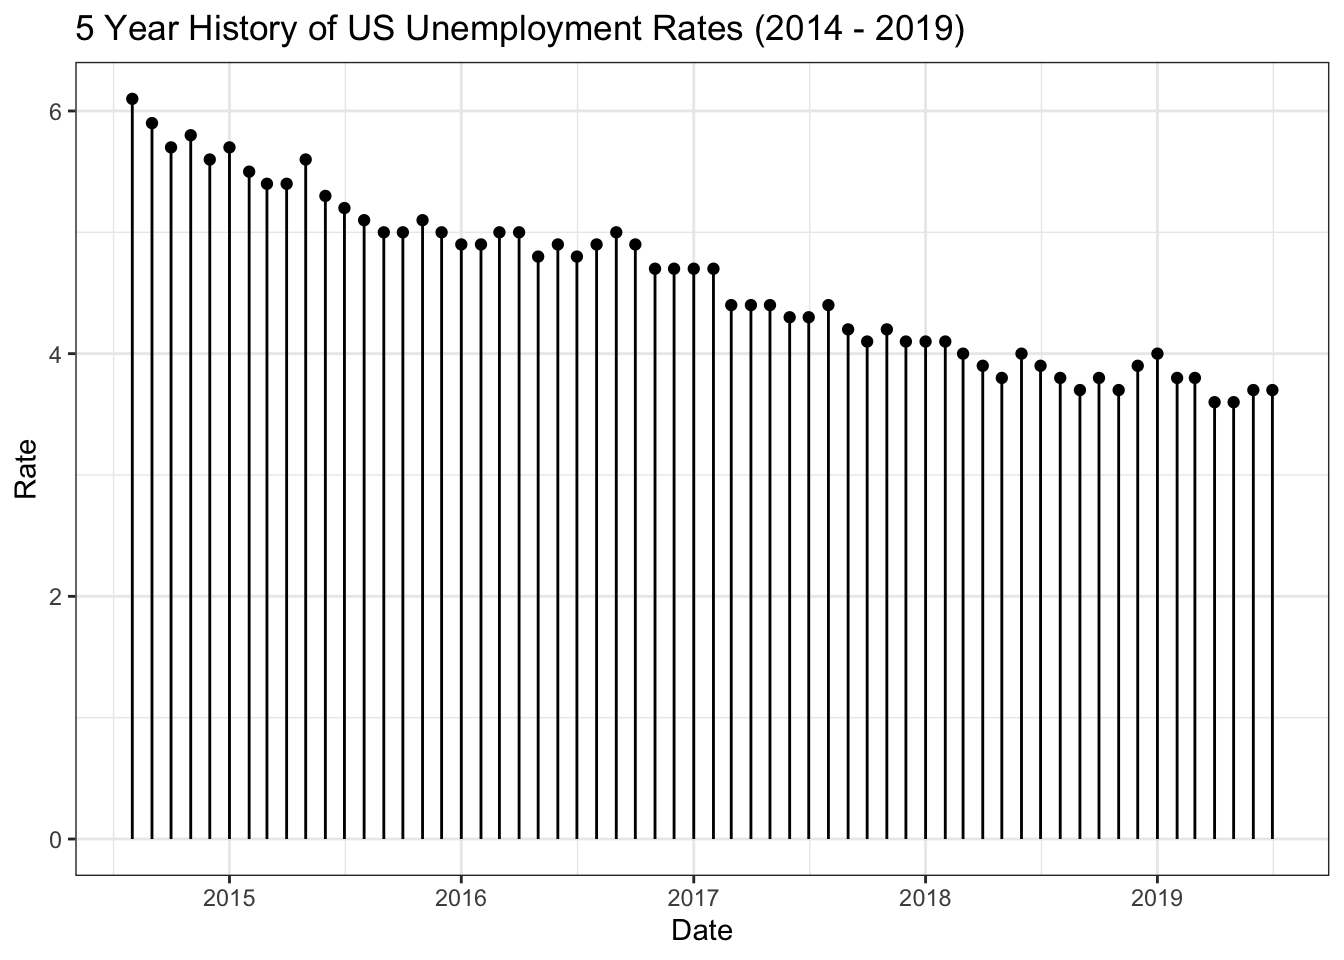
\includegraphics{gggallery_files/figure-latex/unnamed-chunk-38-1.pdf}

\hypertarget{lex}{%
\chapter*{Global life expectancy: Line chart}\label{lex}}
\addcontentsline{toc}{chapter}{Global life expectancy: Line chart}

\hypertarget{lexdata}{%
\subsubsection*{Data}\label{lexdata}}
\addcontentsline{toc}{subsubsection}{Data}

This plot uses the \emph{life\_ex} data frame of the \emph{gcubed} package. This data frame contains life expectancy data for numerous countries and groups of countries in the \emph{Entity} column.

\begin{Shaded}
\begin{Highlighting}[]
\KeywordTok{head}\NormalTok{(life_ex)}
\end{Highlighting}
\end{Shaded}

\begin{verbatim}
## # A tibble: 6 x 4
##   Entity      Code   Year    LE
##   <chr>       <chr> <dbl> <dbl>
## 1 Afghanistan AFG    1950  27.5
## 2 Afghanistan AFG    1951  27.8
## 3 Afghanistan AFG    1952  28.4
## 4 Afghanistan AFG    1953  28.9
## 5 Afghanistan AFG    1954  29.4
## 6 Afghanistan AFG    1955  29.9
\end{verbatim}

\hypertarget{lexcode}{%
\subsubsection*{Code for plot}\label{lexcode}}
\addcontentsline{toc}{subsubsection}{Code for plot}

First, we will restrict the data set to only those rows that contain the life expectancy values for the country groups we are interested in. (Note that this filtering of rows could also have been done using base R.)

\begin{Shaded}
\begin{Highlighting}[]
\NormalTok{groups <-}\StringTok{ }\KeywordTok{c}\NormalTok{(}\StringTok{"Upper-middle-income countries"}\NormalTok{, }\StringTok{"Middle-income countries"}\NormalTok{, }\StringTok{"Low-income countries"}\NormalTok{,}
  \StringTok{"Lower-middle-income countries"}\NormalTok{,}\StringTok{"High-income countries"}\NormalTok{)}

\KeywordTok{library}\NormalTok{(dplyr)}
\NormalTok{df <-}\StringTok{ }\KeywordTok{filter}\NormalTok{(life_ex, Entity }\OperatorTok\StringTok{ }\NormalTok{groups)}
\KeywordTok{head}\NormalTok{(df)}
\end{Highlighting}
\end{Shaded}

\begin{verbatim}
## # A tibble: 6 x 4
##   Entity                Code   Year    LE
##   <chr>                 <chr> <dbl> <dbl>
## 1 High-income countries <NA>   1950  64.3
## 2 High-income countries <NA>   1951  64.6
## 3 High-income countries <NA>   1952  65.1
## 4 High-income countries <NA>   1953  65.5
## 5 High-income countries <NA>   1954  66.0
## 6 High-income countries <NA>   1955  66.4
\end{verbatim}

The data is already in the correct shape to be used by \emph{geom\_line}: all the life expectancy values are in the single column, \emph{LE}.
To get different lines for each income group, the \emph{group} aesthetic is used in the creation of the \emph{ggplot} object. To give each line a different colour, the \emph{colour} aesthetic is used.

\begin{Shaded}
\begin{Highlighting}[]
\NormalTok{le_plt <-}\StringTok{ }\KeywordTok{ggplot}\NormalTok{(df, }\KeywordTok{aes}\NormalTok{(}\DataTypeTok{x =}\NormalTok{ Year, }\DataTypeTok{y =}\NormalTok{ LE, }\DataTypeTok{group =}\NormalTok{ Entity, }\DataTypeTok{colour =}\NormalTok{ Entity)) }\OperatorTok{+}\StringTok{ }
\StringTok{  }\KeywordTok{geom_line}\NormalTok{() }\OperatorTok{+}\StringTok{ }
\StringTok{  }\KeywordTok{ylab}\NormalTok{(}\StringTok{"Life Expectancy (Years)"}\NormalTok{) }\OperatorTok{+}\StringTok{ }
\StringTok{  }\KeywordTok{ggtitle}\NormalTok{(}\StringTok{"Global Life Expectancy (1960 - 2015)"}\NormalTok{) }\OperatorTok{+}
\StringTok{  }\KeywordTok{theme}\NormalTok{(}\DataTypeTok{legend.title =} \KeywordTok{element_blank}\NormalTok{())}

\NormalTok{le_plt}
\end{Highlighting}
\end{Shaded}

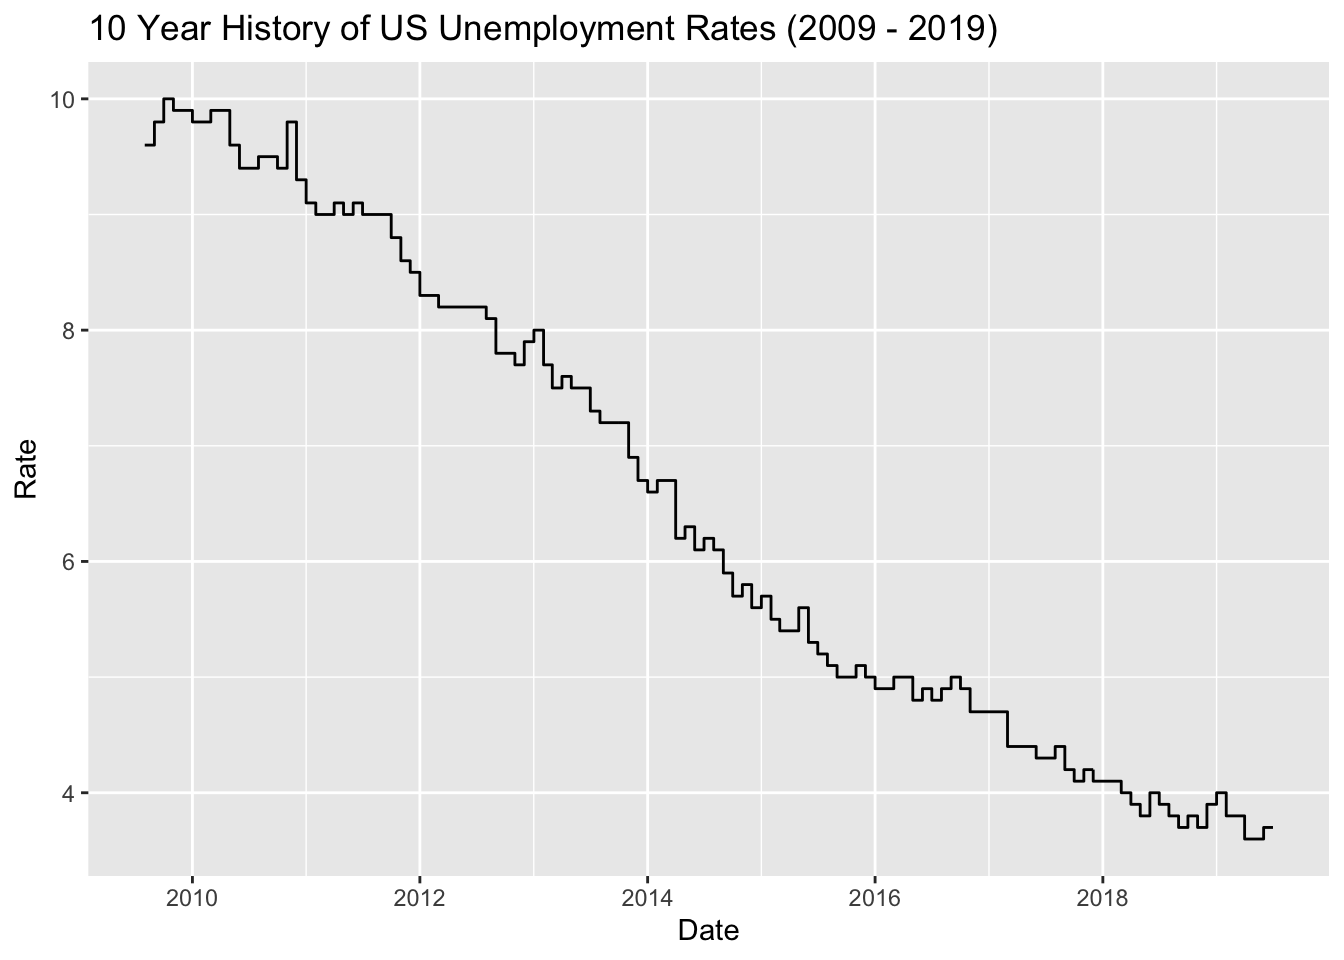
\includegraphics{gggallery_files/figure-latex/unnamed-chunk-42-1.pdf}

We can reorder the country groups so that the legend shows in the same order that the lines do in the plot.

\begin{Shaded}
\begin{Highlighting}[]
\NormalTok{group_order <-}\StringTok{ }\KeywordTok{c}\NormalTok{(}\StringTok{"High-income countries"}\NormalTok{,  }\StringTok{"Upper-middle-income countries"}\NormalTok{, }\StringTok{"Middle-income countries"}\NormalTok{,}\StringTok{"Lower-middle-income countries"}\NormalTok{, }\StringTok{"Low-income countries"}\NormalTok{)}

\NormalTok{df}\OperatorTok{$}\NormalTok{Entity <-}\StringTok{ }\KeywordTok{factor}\NormalTok{(df}\OperatorTok{$}\NormalTok{Entity, }\DataTypeTok{levels =}\NormalTok{ group_order)}

\NormalTok{le_plt <-}\StringTok{ }\KeywordTok{ggplot}\NormalTok{(df, }\KeywordTok{aes}\NormalTok{(}\DataTypeTok{x =}\NormalTok{ Year, }\DataTypeTok{y =}\NormalTok{ LE, }\DataTypeTok{group =}\NormalTok{ Entity, }\DataTypeTok{colour =}\NormalTok{ Entity)) }\OperatorTok{+}\StringTok{ }
\StringTok{  }\KeywordTok{geom_line}\NormalTok{() }\OperatorTok{+}\StringTok{ }
\StringTok{  }\KeywordTok{ylab}\NormalTok{(}\StringTok{"Life Expectancy (Years)"}\NormalTok{) }\OperatorTok{+}\StringTok{ }
\StringTok{  }\KeywordTok{ggtitle}\NormalTok{(}\StringTok{"Global Life Expectancy (1960 - 2015)"}\NormalTok{) }\OperatorTok{+}
\StringTok{  }\KeywordTok{theme}\NormalTok{(}\DataTypeTok{legend.title =} \KeywordTok{element_blank}\NormalTok{())}

\NormalTok{le_plt }
\end{Highlighting}
\end{Shaded}

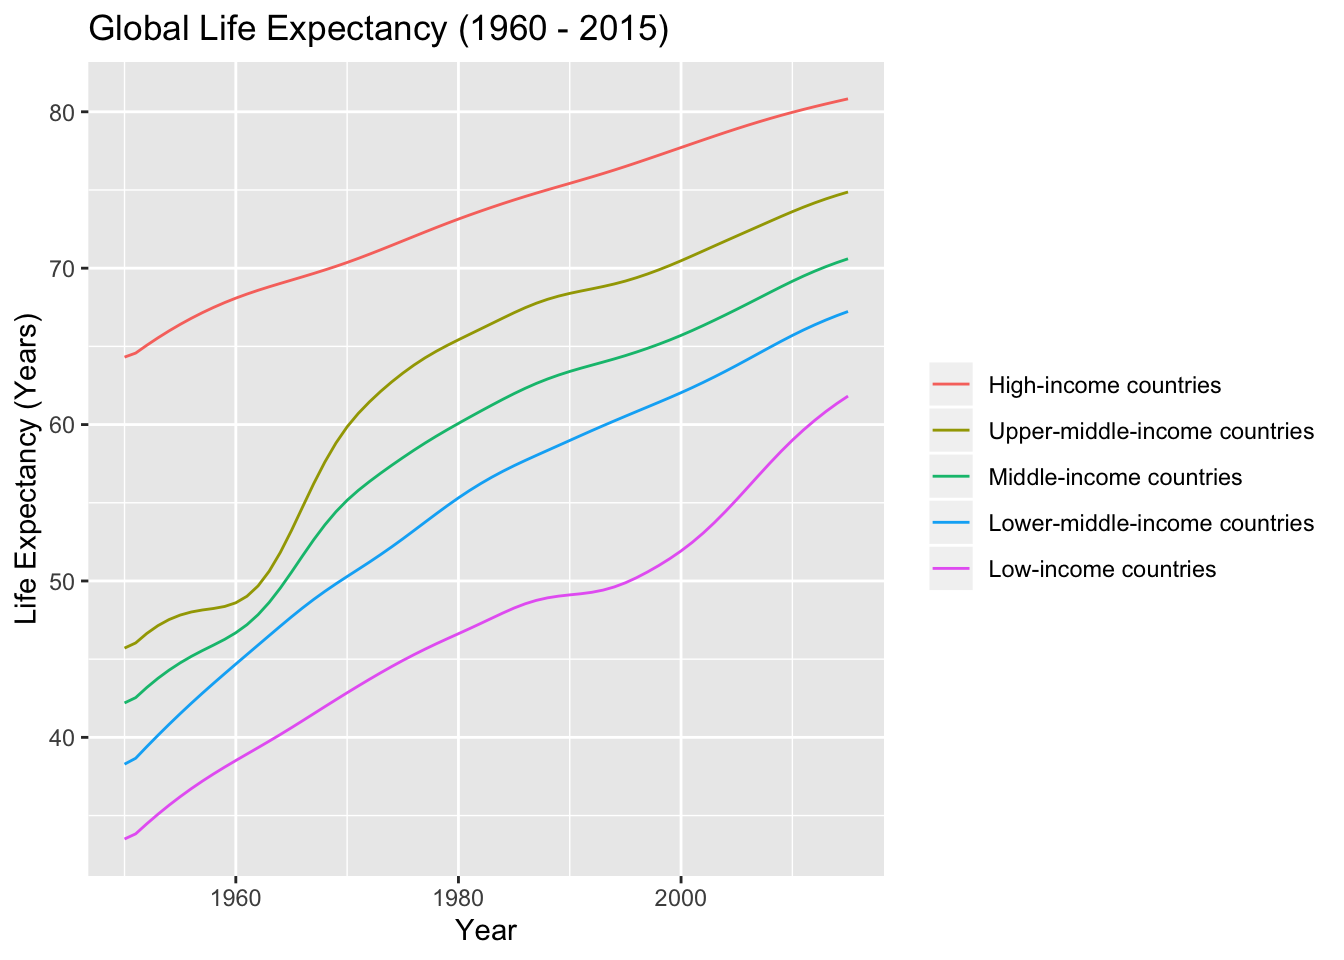
\includegraphics{gggallery_files/figure-latex/unnamed-chunk-43-1.pdf}

\hypertarget{apple}{%
\chapter*{Apple Inc Revenue}\label{apple}}
\addcontentsline{toc}{chapter}{Apple Inc Revenue}

\hypertarget{appledata}{%
\subsubsection*{Data}\label{appledata}}
\addcontentsline{toc}{subsubsection}{Data}

This plot uses the \emph{apple} data frame of the \emph{gcubed} package. This data frame contains the revenue (in millions of dollars) for each of Apple's product lines for the period 2015 to 2018.

\begin{Shaded}
\begin{Highlighting}[]
\KeywordTok{head}\NormalTok{(apple)}
\end{Highlighting}
\end{Shaded}

\begin{verbatim}
## # A tibble: 6 x 5
##    Year Quarter Product        Units Revenue
##   <int>   <int> <chr>          <dbl>   <dbl>
## 1  2015       1 iPad           21419    8985
## 2  2015       1 iPhone         74468   51182
## 3  2015       1 Mac             5519    6944
## 4  2015       1 Other Products    NA    2689
## 5  2015       1 Services          NA    4799
## 6  2015       2 iPad           12623    5428
\end{verbatim}

\hypertarget{applecode}{%
\subsubsection*{Code for plot}\label{applecode}}
\addcontentsline{toc}{subsubsection}{Code for plot}

The code makes use of both \emph{geom\_point} and \emph{geom\_line} as well as \emph{group} and \emph{colour} aesthetics.

\begin{Shaded}
\begin{Highlighting}[]
\KeywordTok{library}\NormalTok{(ggplot2)}
\KeywordTok{library}\NormalTok{(scales) }\CommentTok{#for formatting the numerical y-axis values}

\NormalTok{apple_rev_plot <-}\StringTok{ }\KeywordTok{ggplot}\NormalTok{(}\DataTypeTok{data =}\NormalTok{ apple, }\KeywordTok{aes}\NormalTok{(}\DataTypeTok{x =} \KeywordTok{paste}\NormalTok{(Year, Quarter, }\DataTypeTok{sep =} \StringTok{" Q"}\NormalTok{), }\DataTypeTok{y =}\NormalTok{ Revenue, }\DataTypeTok{group =}\NormalTok{ Product, }\DataTypeTok{colour =}\NormalTok{ Product)) }\OperatorTok{+}\StringTok{ }
\StringTok{  }\KeywordTok{geom_point}\NormalTok{() }\OperatorTok{+}
\StringTok{  }\KeywordTok{geom_line}\NormalTok{() }\OperatorTok{+}\StringTok{ }
\StringTok{  }\KeywordTok{ggtitle}\NormalTok{(}\StringTok{"Apple Inc. Revenue (2015 - 2018)"}\NormalTok{) }\OperatorTok{+}\StringTok{ }
\StringTok{  }\KeywordTok{ylab}\NormalTok{(}\StringTok{"Revenue (millions of $)"}\NormalTok{) }\OperatorTok{+}
\StringTok{  }\KeywordTok{theme_bw}\NormalTok{() }\OperatorTok{+}\StringTok{ }
\StringTok{  }\KeywordTok{scale_y_continuous}\NormalTok{(}\DataTypeTok{label=}\NormalTok{comma) }\OperatorTok{+}\StringTok{ }
\StringTok{  }\KeywordTok{theme}\NormalTok{(}\DataTypeTok{axis.text.x =} \KeywordTok{element_text}\NormalTok{(}\DataTypeTok{angle =} \DecValTok{90}\NormalTok{),}
        \DataTypeTok{axis.title.x =} \KeywordTok{element_blank}\NormalTok{(),}
        \DataTypeTok{plot.title =} \KeywordTok{element_text}\NormalTok{(}\DataTypeTok{size =} \DecValTok{16}\NormalTok{, }\DataTypeTok{face =} \StringTok{"bold"}\NormalTok{, }\DataTypeTok{hjust =} \FloatTok{0.5}\NormalTok{))}

\NormalTok{apple_rev_plot}
\end{Highlighting}
\end{Shaded}

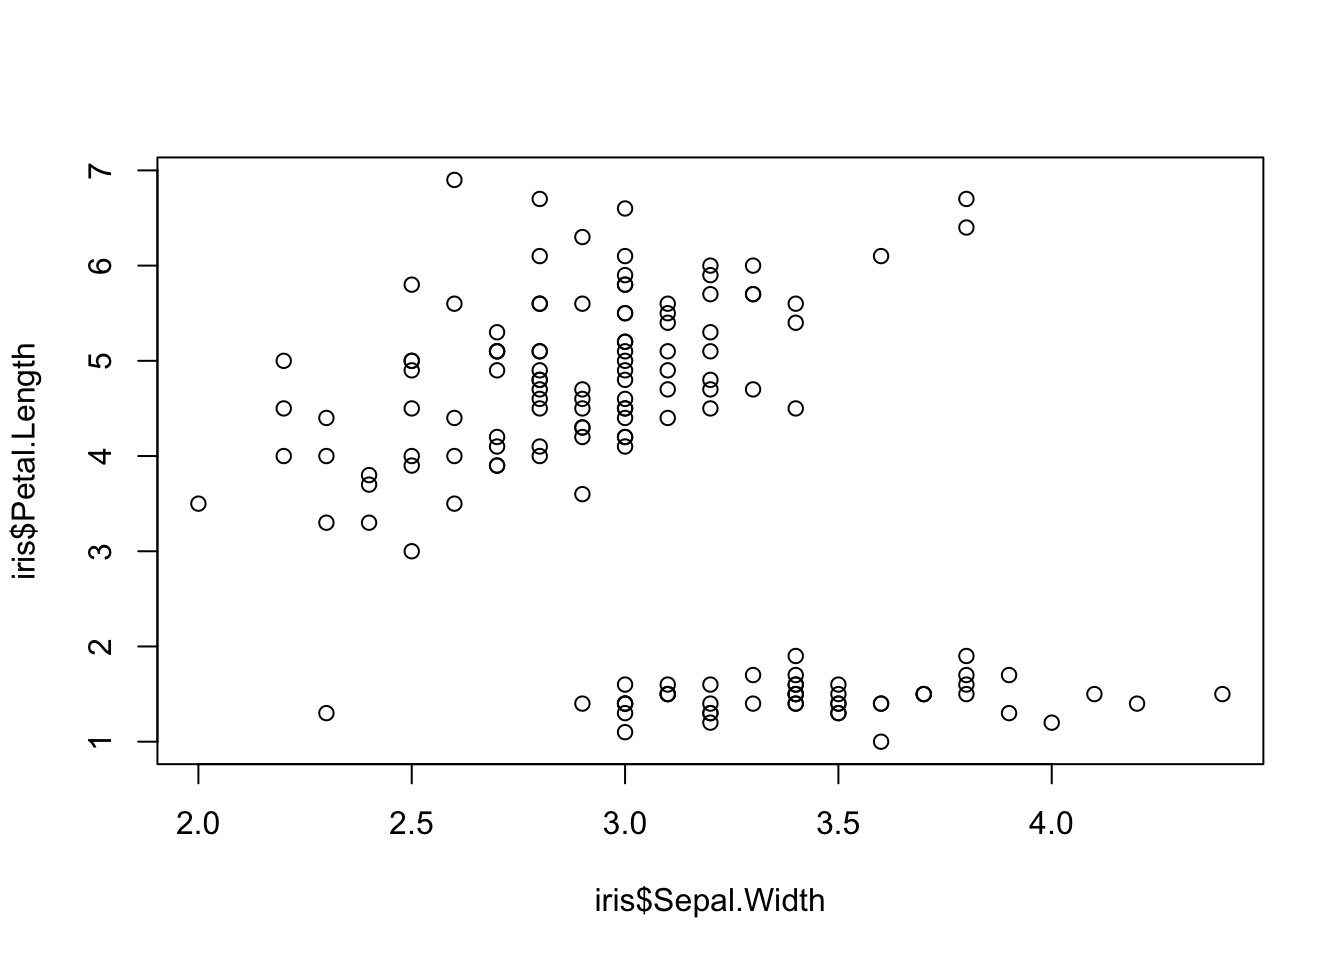
\includegraphics{gggallery_files/figure-latex/unnamed-chunk-46-1.pdf}

\hypertarget{budget}{%
\chapter*{Budget Surplus or Deficit}\label{budget}}
\addcontentsline{toc}{chapter}{Budget Surplus or Deficit}

\hypertarget{budgetdata}{%
\subsubsection*{Data}\label{budgetdata}}
\addcontentsline{toc}{subsubsection}{Data}

This plot uses the \emph{budget} data frame of the \emph{gcubed} package. In particular, the columns \emph{Year} and \emph{SurpDef\_pg} are used. \emph{SurpDef\_pg} represents the surplus/deficit as a percentage of the US GDP for the given year. Some rows of the data frame are shown below.

\begin{Shaded}
\begin{Highlighting}[]
\NormalTok{budget[budget}\OperatorTok{$}\NormalTok{Year }\OperatorTok\StringTok{ }\KeywordTok{c}\NormalTok{(}\DecValTok{1970}\NormalTok{, }\DecValTok{1980}\NormalTok{, }\DecValTok{1990}\NormalTok{, }\DecValTok{2000}\NormalTok{, }\DecValTok{2010}\NormalTok{),}
       \KeywordTok{c}\NormalTok{(}\StringTok{"Year"}\NormalTok{, }\StringTok{"SurpDef_pg"}\NormalTok{)]}
\end{Highlighting}
\end{Shaded}

\begin{verbatim}
## # A tibble: 5 x 2
##    Year SurpDef_pg
##   <dbl>      <dbl>
## 1  1970       -0.3
## 2  1980       -2.6
## 3  1990       -3.7
## 4  2000        2.3
## 5  2010       -8.7
\end{verbatim}

\hypertarget{budgetcode}{%
\subsubsection*{Code}\label{budgetcode}}
\addcontentsline{toc}{subsubsection}{Code}

First, we make a plot using \emph{geom\_line}. \emph{geom\_hline} is also used to create the x-axis.

\begin{Shaded}
\begin{Highlighting}[]
\NormalTok{df <-}\StringTok{ }\NormalTok{budget[budget}\OperatorTok{$}\NormalTok{Year }\OperatorTok{>=}\StringTok{ }\DecValTok{1950}\NormalTok{, ]}

\NormalTok{budget_plt <-}\StringTok{ }\KeywordTok{ggplot}\NormalTok{(}\DataTypeTok{data =}\NormalTok{ df, }\KeywordTok{aes}\NormalTok{(}\DataTypeTok{x =}\NormalTok{ Year, }\DataTypeTok{y =}\NormalTok{ SurpDef_pg)) }\OperatorTok{+}\StringTok{ }
\StringTok{  }\KeywordTok{geom_line}\NormalTok{() }\OperatorTok{+}\StringTok{ }
\StringTok{  }\KeywordTok{geom_hline}\NormalTok{(}\DataTypeTok{yintercept =} \DecValTok{0}\NormalTok{) }\OperatorTok{+}\StringTok{ }\CommentTok{#deficit ribbon below}
\StringTok{  }\KeywordTok{theme_bw}\NormalTok{() }\OperatorTok{+}\StringTok{  }
\StringTok{  }\KeywordTok{ylab}\NormalTok{(}\StringTok{"Surplus or Deficit (% of GDP)"}\NormalTok{) }\OperatorTok{+}\StringTok{ }
\StringTok{  }\KeywordTok{ggtitle}\NormalTok{(}\StringTok{"US Federal Budget (1950 - 2018) "}\NormalTok{) }\OperatorTok{+}\StringTok{ }
\StringTok{    }\KeywordTok{theme}\NormalTok{(}\DataTypeTok{panel.grid.minor =} \KeywordTok{element_blank}\NormalTok{(), }
        \DataTypeTok{axis.text.x =} \KeywordTok{element_text}\NormalTok{(}\DataTypeTok{angle =} \DecValTok{90}\NormalTok{), }
        \DataTypeTok{plot.title =} \KeywordTok{element_text}\NormalTok{(}\DataTypeTok{size =} \DecValTok{20}\NormalTok{, }\DataTypeTok{face =} \StringTok{"bold"}\NormalTok{, }\DataTypeTok{hjust =} \FloatTok{0.5}\NormalTok{),}
        \DataTypeTok{legend.title =} \KeywordTok{element_blank}\NormalTok{())}

\NormalTok{budget_plt }
\end{Highlighting}
\end{Shaded}

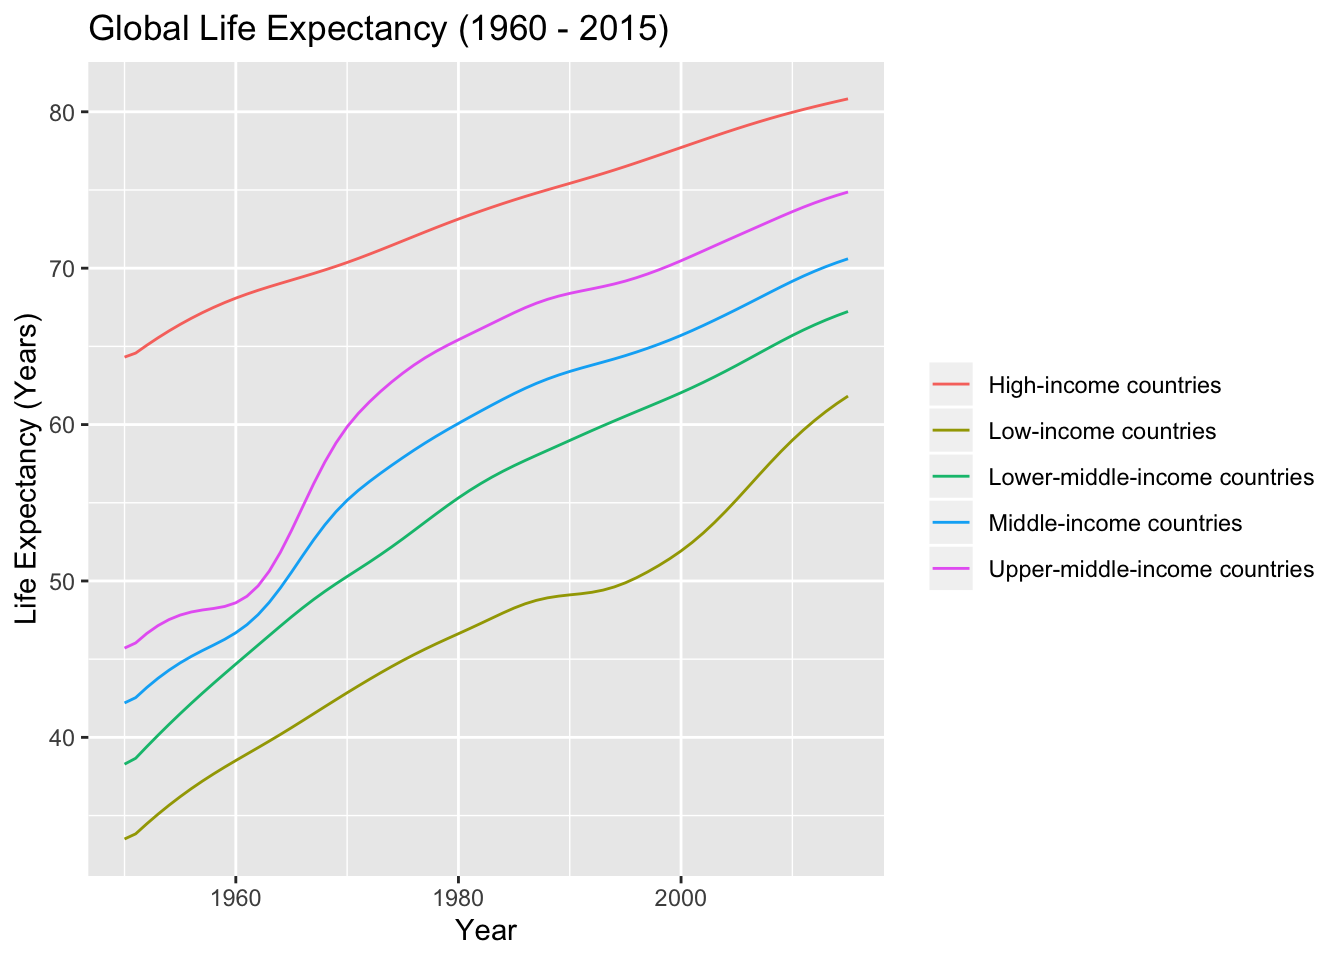
\includegraphics{gggallery_files/figure-latex/unnamed-chunk-49-1.pdf}

The filled-in regions are added using the \emph{geom\_ribbon} geometry.

\begin{Shaded}
\begin{Highlighting}[]
\NormalTok{budget_plt <-}\StringTok{ }\NormalTok{budget_plt }\OperatorTok{+}\StringTok{ }
\StringTok{  }\KeywordTok{geom_ribbon}\NormalTok{(}\KeywordTok{aes}\NormalTok{(}\DataTypeTok{ymin =} \KeywordTok{ifelse}\NormalTok{(SurpDef_pg }\OperatorTok{<}\StringTok{ }\DecValTok{0}\NormalTok{, SurpDef_pg, }\DecValTok{0}\NormalTok{), }
                  \DataTypeTok{ymax =} \DecValTok{0}\NormalTok{, }
                  \DataTypeTok{fill =} \StringTok{"Deficit"}\NormalTok{), }\DataTypeTok{alpha =} \FloatTok{0.2}\NormalTok{) }\OperatorTok{+}
\StringTok{  }\KeywordTok{geom_ribbon}\NormalTok{(}\KeywordTok{aes}\NormalTok{(}\DataTypeTok{ymin =} \DecValTok{0}\NormalTok{,}
                  \DataTypeTok{ymax =} \KeywordTok{ifelse}\NormalTok{(SurpDef_pg }\OperatorTok{>}\StringTok{ }\DecValTok{0}\NormalTok{, SurpDef_pg, }\DecValTok{0}\NormalTok{), }
                  \DataTypeTok{fill =} \StringTok{"Surplus"}\NormalTok{), }\DataTypeTok{alpha =} \FloatTok{0.2}\NormalTok{) }
  

\NormalTok{budget_plt}
\end{Highlighting}
\end{Shaded}

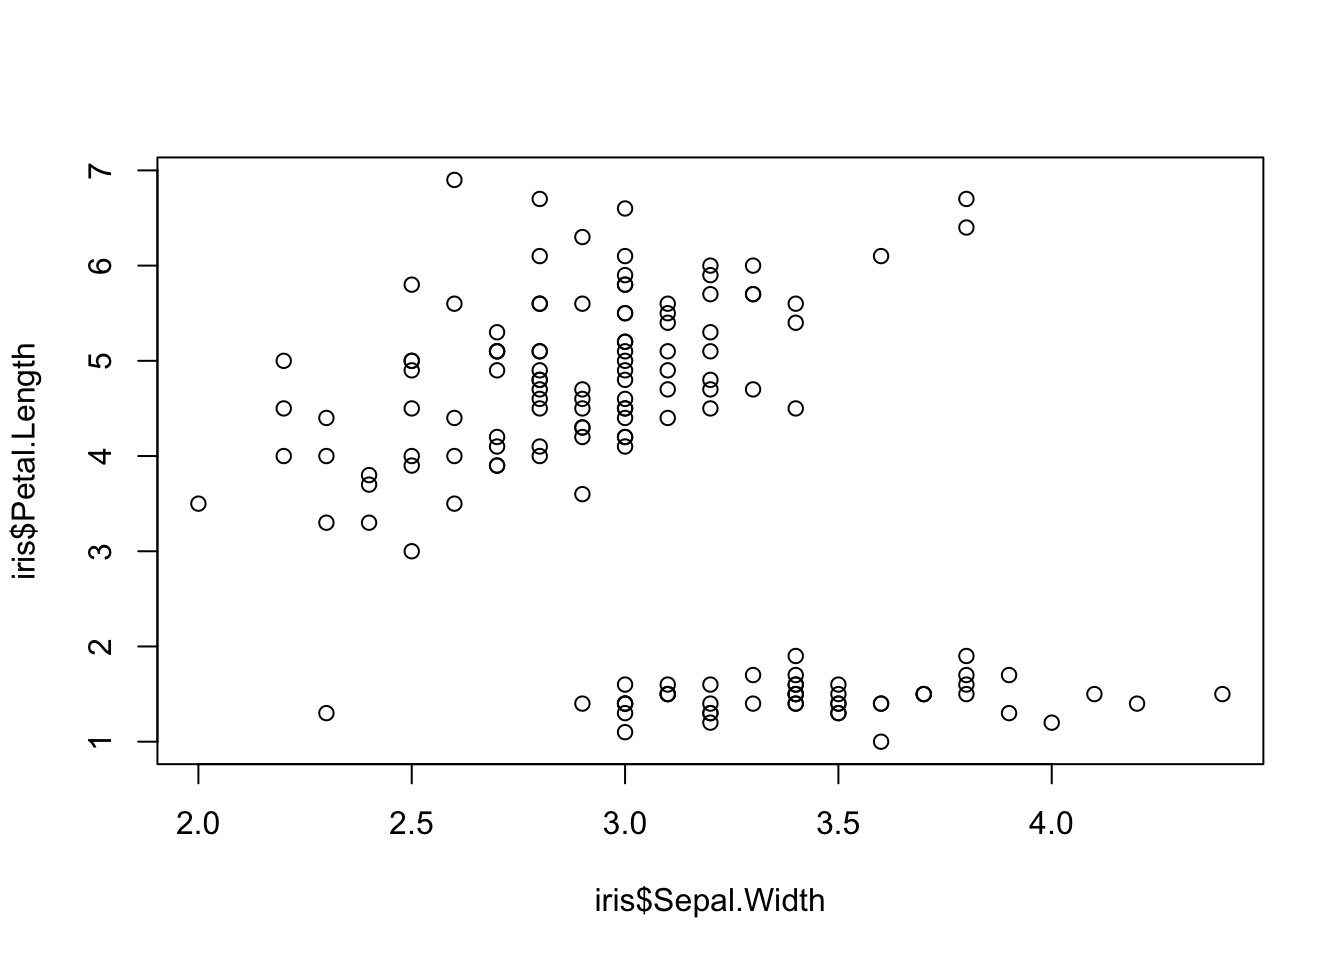
\includegraphics{gggallery_files/figure-latex/unnamed-chunk-50-1.pdf}

Alternatively, all the code for the entire plot is shown below.

\begin{Shaded}
\begin{Highlighting}[]
\NormalTok{budget_plt <-}\StringTok{ }\KeywordTok{ggplot}\NormalTok{(}\DataTypeTok{data =}\NormalTok{ df, }\KeywordTok{aes}\NormalTok{(}\DataTypeTok{x =}\NormalTok{ Year, }\DataTypeTok{y =}\NormalTok{ SurpDef_pg)) }\OperatorTok{+}\StringTok{ }
\StringTok{  }\KeywordTok{geom_line}\NormalTok{() }\OperatorTok{+}\StringTok{ }
\StringTok{  }\KeywordTok{geom_hline}\NormalTok{(}\DataTypeTok{yintercept =} \DecValTok{0}\NormalTok{) }\OperatorTok{+}\StringTok{ }\CommentTok{#deficit ribbon below}
\StringTok{  }\KeywordTok{theme_bw}\NormalTok{() }\OperatorTok{+}\StringTok{  }
\StringTok{  }\KeywordTok{ylab}\NormalTok{(}\StringTok{"Surplus or Deficit (% of GDP)"}\NormalTok{) }\OperatorTok{+}\StringTok{ }
\StringTok{  }\KeywordTok{ggtitle}\NormalTok{(}\StringTok{"US Federal Budget (1950 - 2018) "}\NormalTok{) }\OperatorTok{+}\StringTok{ }
\StringTok{    }\KeywordTok{theme}\NormalTok{(}\DataTypeTok{panel.grid.minor =} \KeywordTok{element_blank}\NormalTok{(), }
        \DataTypeTok{axis.text.x =} \KeywordTok{element_text}\NormalTok{(}\DataTypeTok{angle =} \DecValTok{90}\NormalTok{), }
        \DataTypeTok{plot.title =} \KeywordTok{element_text}\NormalTok{(}\DataTypeTok{size =} \DecValTok{20}\NormalTok{, }\DataTypeTok{face =} \StringTok{"bold"}\NormalTok{, }\DataTypeTok{hjust =} \FloatTok{0.5}\NormalTok{),}
        \DataTypeTok{legend.title =} \KeywordTok{element_blank}\NormalTok{()) }\OperatorTok{+}\StringTok{ }
\StringTok{  }\KeywordTok{geom_ribbon}\NormalTok{(}\KeywordTok{aes}\NormalTok{(}\DataTypeTok{ymin =} \KeywordTok{ifelse}\NormalTok{(SurpDef_pg }\OperatorTok{<}\StringTok{ }\DecValTok{0}\NormalTok{, SurpDef_pg, }\DecValTok{0}\NormalTok{), }
                  \DataTypeTok{ymax =} \DecValTok{0}\NormalTok{, }
                  \DataTypeTok{fill =} \StringTok{"Deficit"}\NormalTok{), }\DataTypeTok{alpha =} \FloatTok{0.2}\NormalTok{) }\OperatorTok{+}
\StringTok{  }\KeywordTok{geom_ribbon}\NormalTok{(}\KeywordTok{aes}\NormalTok{(}\DataTypeTok{ymin =} \DecValTok{0}\NormalTok{,}
                  \DataTypeTok{ymax =} \KeywordTok{ifelse}\NormalTok{(SurpDef_pg }\OperatorTok{>}\StringTok{ }\DecValTok{0}\NormalTok{, SurpDef_pg, }\DecValTok{0}\NormalTok{), }
                  \DataTypeTok{fill =} \StringTok{"Surplus"}\NormalTok{), }\DataTypeTok{alpha =} \FloatTok{0.2}\NormalTok{) }
\end{Highlighting}
\end{Shaded}

\hypertarget{atp}{%
\chapter*{2 Year History of Top-ranked ATP Players}\label{atp}}
\addcontentsline{toc}{chapter}{2 Year History of Top-ranked ATP Players}

\hypertarget{atpdata}{%
\subsubsection*{Data}\label{atpdata}}
\addcontentsline{toc}{subsubsection}{Data}

For this plot, we will use the \emph{atp\_rankings} data frame of the \emph{gcubed} package.

\begin{Shaded}
\begin{Highlighting}[]
\KeywordTok{head}\NormalTok{(atp_rankings)}
\end{Highlighting}
\end{Shaded}

\begin{verbatim}
## # A tibble: 6 x 6
##    Year Month   Day Singles Player    Date               
##   <dbl> <dbl> <dbl>   <int> <chr>     <dttm>             
## 1  2017     8     7       5 Djokovic  2017-08-07 12:00:00
## 2  2017     8     7       2 Nadal     2017-08-07 12:00:00
## 3  2017     8     7       3 Federer   2017-08-07 12:00:00
## 4  2017     8     7       7 Thiem     2017-08-07 12:00:00
## 5  2017     8     7     168 Tsitsipas 2017-08-07 12:00:00
## 6  2017     8    14       5 Djokovic  2017-08-14 12:00:00
\end{verbatim}

First, create a new variable, \emph{Ranking} that preserves the rankings when the player is in the top 10. When the player is not in the top 10, the new variable is set to: 11 if the player is in the top 20; 12 if the player is ranked between 21 and 50 (inclusive); 13 if the player is ranked between 51 and 100 (inclusive); 14 if the player is ranked lower than 100.

Also, we create a variable \emph{Change} to be used later to identify the points in time when the players' rankings changed.

\begin{Shaded}
\begin{Highlighting}[]
\NormalTok{rankings <-}\StringTok{ }\KeywordTok{mutate}\NormalTok{(atp_rankings, }\DataTypeTok{Ranking =} \KeywordTok{ifelse}\NormalTok{(Singles }\OperatorTok{>}\StringTok{ }\DecValTok{100}\NormalTok{, }\DecValTok{14}\NormalTok{, }
                          \KeywordTok{ifelse}\NormalTok{(Singles }\OperatorTok{>}\StringTok{ }\DecValTok{50}\NormalTok{, }\DecValTok{13}\NormalTok{, }
                                 \KeywordTok{ifelse}\NormalTok{(Singles }\OperatorTok{>}\StringTok{ }\DecValTok{20}\NormalTok{, }\DecValTok{12}\NormalTok{, }
                                        \KeywordTok{ifelse}\NormalTok{(Singles }\OperatorTok{>}\StringTok{ }\DecValTok{10}\NormalTok{, }\DecValTok{11}\NormalTok{, Singles))))) }\OperatorTok
\StringTok{  }\KeywordTok{group_by}\NormalTok{(Player) }\OperatorTok\StringTok{ }\KeywordTok{mutate}\NormalTok{(}\DataTypeTok{Change =} \KeywordTok{c}\NormalTok{(}\DecValTok{0}\NormalTok{,}\KeywordTok{diff}\NormalTok{(Ranking))) }\OperatorTok\StringTok{ }\KeywordTok{ungroup}\NormalTok{()}
\end{Highlighting}
\end{Shaded}

\hypertarget{atpcode}{%
\subsubsection*{Code for plot}\label{atpcode}}
\addcontentsline{toc}{subsubsection}{Code for plot}

\begin{Shaded}
\begin{Highlighting}[]
\NormalTok{ylabels <-}\StringTok{ }\KeywordTok{c}\NormalTok{(}\DecValTok{1}\OperatorTok{:}\DecValTok{10}\NormalTok{, }\StringTok{"Top 20"}\NormalTok{, }\StringTok{"Top 50"}\NormalTok{, }\StringTok{"Top 100"}\NormalTok{, }\StringTok{"Out of Top 100"}\NormalTok{)}


\NormalTok{show_date <-}\StringTok{ }\KeywordTok{ISOdate}\NormalTok{(}\DecValTok{2019}\NormalTok{, }\DecValTok{11}\NormalTok{,}\DecValTok{1}\NormalTok{)}
\NormalTok{begin_date <-}\StringTok{ }\KeywordTok{ISOdate}\NormalTok{(}\DecValTok{2017}\NormalTok{, }\DecValTok{8}\NormalTok{, }\DecValTok{7}\NormalTok{)}
\NormalTok{next_date <-}\StringTok{ }\KeywordTok{ISOdate}\NormalTok{(}\DecValTok{2019}\NormalTok{, }\DecValTok{8}\NormalTok{, }\DecValTok{15}\NormalTok{)}


\NormalTok{atp_plt <-}\StringTok{ }\KeywordTok{ggplot}\NormalTok{(}\DataTypeTok{data =}\NormalTok{ rankings, }\KeywordTok{aes}\NormalTok{(}\DataTypeTok{x =}\NormalTok{ Date, }\DataTypeTok{y =}\NormalTok{ Ranking, }\DataTypeTok{group =}\NormalTok{ Player)) }\OperatorTok{+}\StringTok{ }
\StringTok{  }\KeywordTok{geom_line}\NormalTok{(}\KeywordTok{aes}\NormalTok{(}\DataTypeTok{color =}\NormalTok{ Player), }\DataTypeTok{alpha =} \FloatTok{0.4}\NormalTok{, }\DataTypeTok{size =} \FloatTok{1.5}\NormalTok{) }\OperatorTok{+}
\StringTok{  }\KeywordTok{scale_y_continuous}\NormalTok{(}\DataTypeTok{breaks =} \KeywordTok{c}\NormalTok{(}\DecValTok{1}\OperatorTok{:}\DecValTok{14}\NormalTok{), }\DataTypeTok{labels =}\NormalTok{ ylabels, }\DataTypeTok{trans =} \StringTok{"reverse"}\NormalTok{) }\OperatorTok{+}\StringTok{ }
\StringTok{  }\KeywordTok{ggtitle}\NormalTok{(}\StringTok{"2 Year History of Top Ranked ATP Players"}\NormalTok{) }\OperatorTok{+}\StringTok{ }
\StringTok{  }\KeywordTok{xlim}\NormalTok{(}\KeywordTok{c}\NormalTok{(begin_date, show_date)) }\OperatorTok{+}
\StringTok{  }\KeywordTok{theme_bw}\NormalTok{() }

\NormalTok{atp_plt}
\end{Highlighting}
\end{Shaded}

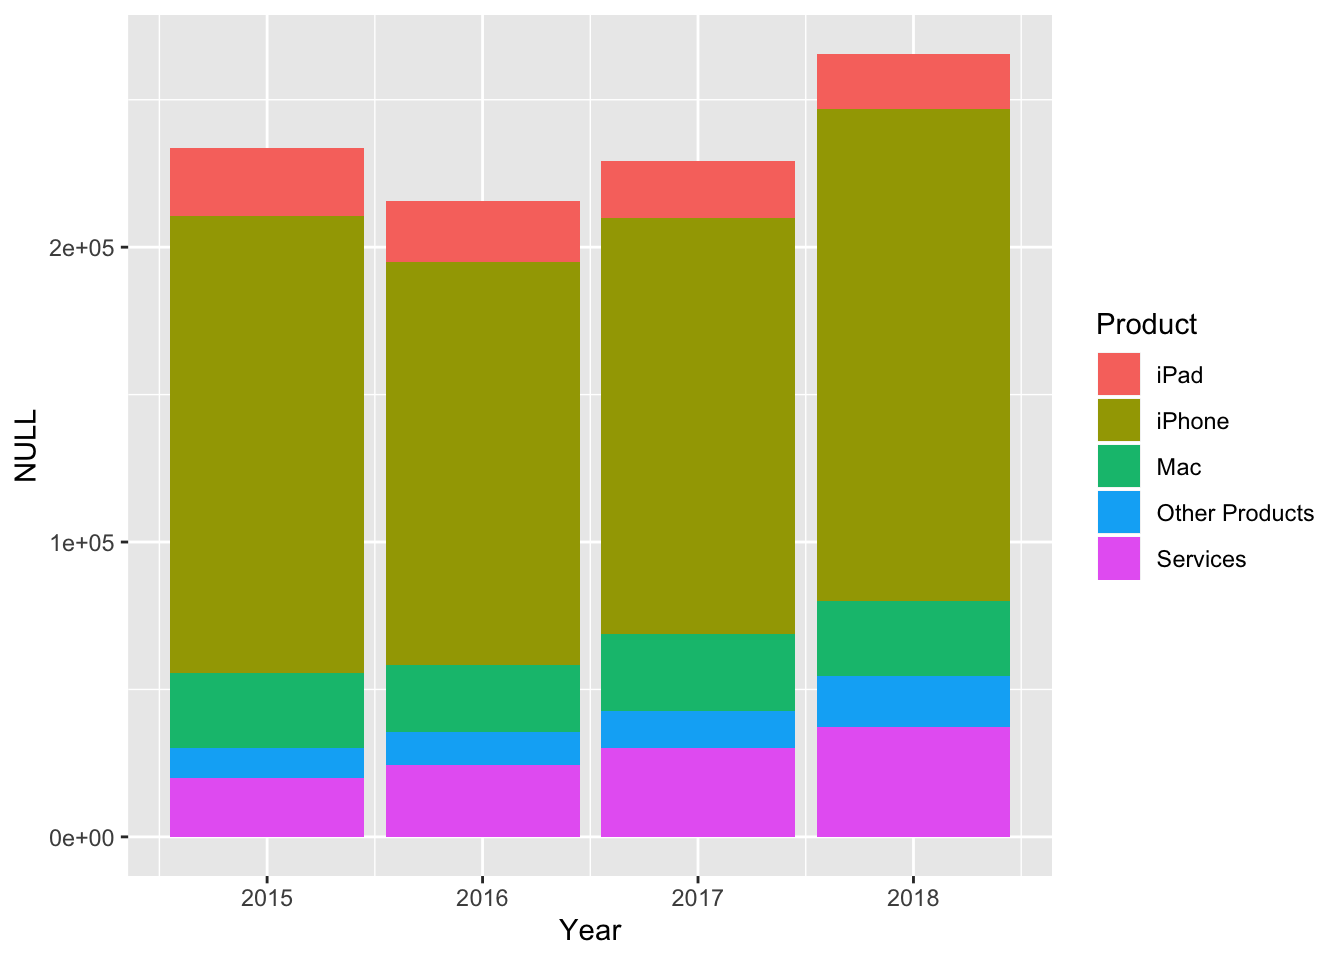
\includegraphics{gggallery_files/figure-latex/unnamed-chunk-55-1.pdf}

Next, we can change the overall look of the plot using the \emph{theme} function to change several
details of the graph.

\begin{Shaded}
\begin{Highlighting}[]
\NormalTok{atp_plt <-}\StringTok{ }\NormalTok{atp_plt }\OperatorTok{+}\StringTok{ }
\StringTok{  }\KeywordTok{theme}\NormalTok{(}\DataTypeTok{panel.grid.major.y =} \KeywordTok{element_blank}\NormalTok{(), }\DataTypeTok{panel.grid.minor.y =} \KeywordTok{element_blank}\NormalTok{(),}
        \DataTypeTok{panel.grid.minor.x =} \KeywordTok{element_blank}\NormalTok{(), }\DataTypeTok{axis.ticks =} \KeywordTok{element_blank}\NormalTok{(), }
        \DataTypeTok{legend.position =} \StringTok{"none"}\NormalTok{, }\DataTypeTok{panel.border =} \KeywordTok{element_blank}\NormalTok{(),}
        \DataTypeTok{axis.title.x =} \KeywordTok{element_blank}\NormalTok{(), }\DataTypeTok{axis.title.y =} \KeywordTok{element_blank}\NormalTok{(),}
        \DataTypeTok{plot.title =} \KeywordTok{element_text}\NormalTok{(}\DataTypeTok{size =} \DecValTok{16}\NormalTok{, }\DataTypeTok{face =} \StringTok{"bold"}\NormalTok{, }\DataTypeTok{hjust =} \FloatTok{0.5}\NormalTok{)) }

\NormalTok{atp_plt}
\end{Highlighting}
\end{Shaded}

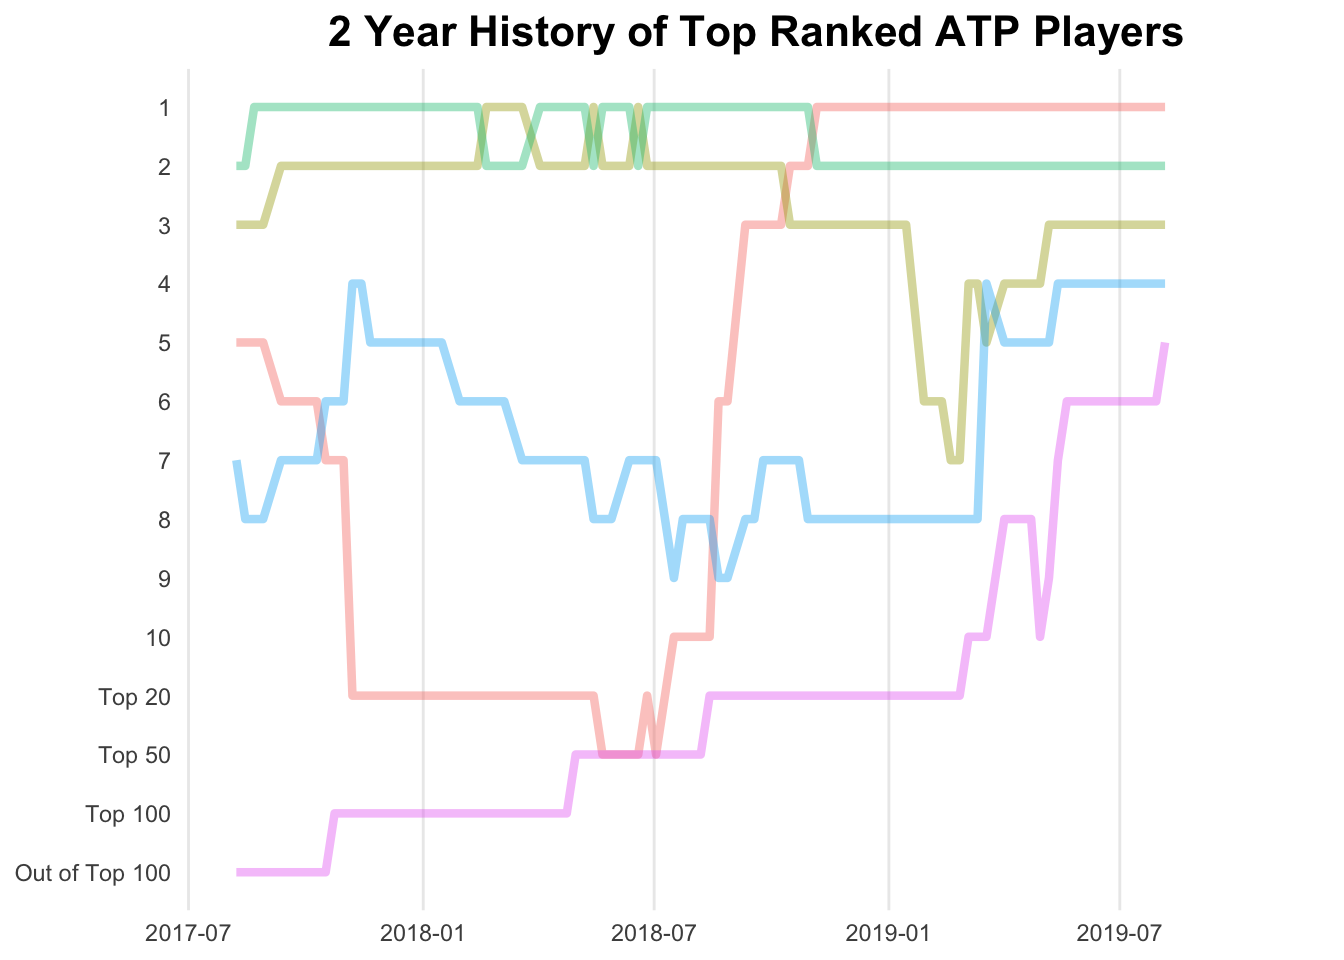
\includegraphics{gggallery_files/figure-latex/unnamed-chunk-56-1.pdf}

Adding some points to signify the times at which the players' rankings changed using \emph{geom\_point}.
We are going to use two \emph{geom\_point} geometries to create a smaller white circle inside the coloured larger circles.

\begin{Shaded}
\begin{Highlighting}[]
\NormalTok{changes <-}\StringTok{ }\KeywordTok{filter}\NormalTok{(rankings, Change }\OperatorTok{!=}\StringTok{ }\DecValTok{0}\NormalTok{)}


\NormalTok{atp_plt <-}\StringTok{ }\NormalTok{atp_plt }\OperatorTok{+}\StringTok{ }\KeywordTok{geom_point}\NormalTok{(}\DataTypeTok{data =}\NormalTok{ changes, }\KeywordTok{aes}\NormalTok{(}\DataTypeTok{x =}\NormalTok{ Date, }\DataTypeTok{y =}\NormalTok{ Ranking, }\DataTypeTok{color =}\NormalTok{ Player)) }\OperatorTok{+}
\StringTok{  }\KeywordTok{geom_point}\NormalTok{(}\DataTypeTok{data =}\NormalTok{ changes, }\DataTypeTok{color =} \StringTok{"#FFFFFF"}\NormalTok{, }\DataTypeTok{size =} \FloatTok{0.25}\NormalTok{) }

\NormalTok{atp_plt}
\end{Highlighting}
\end{Shaded}

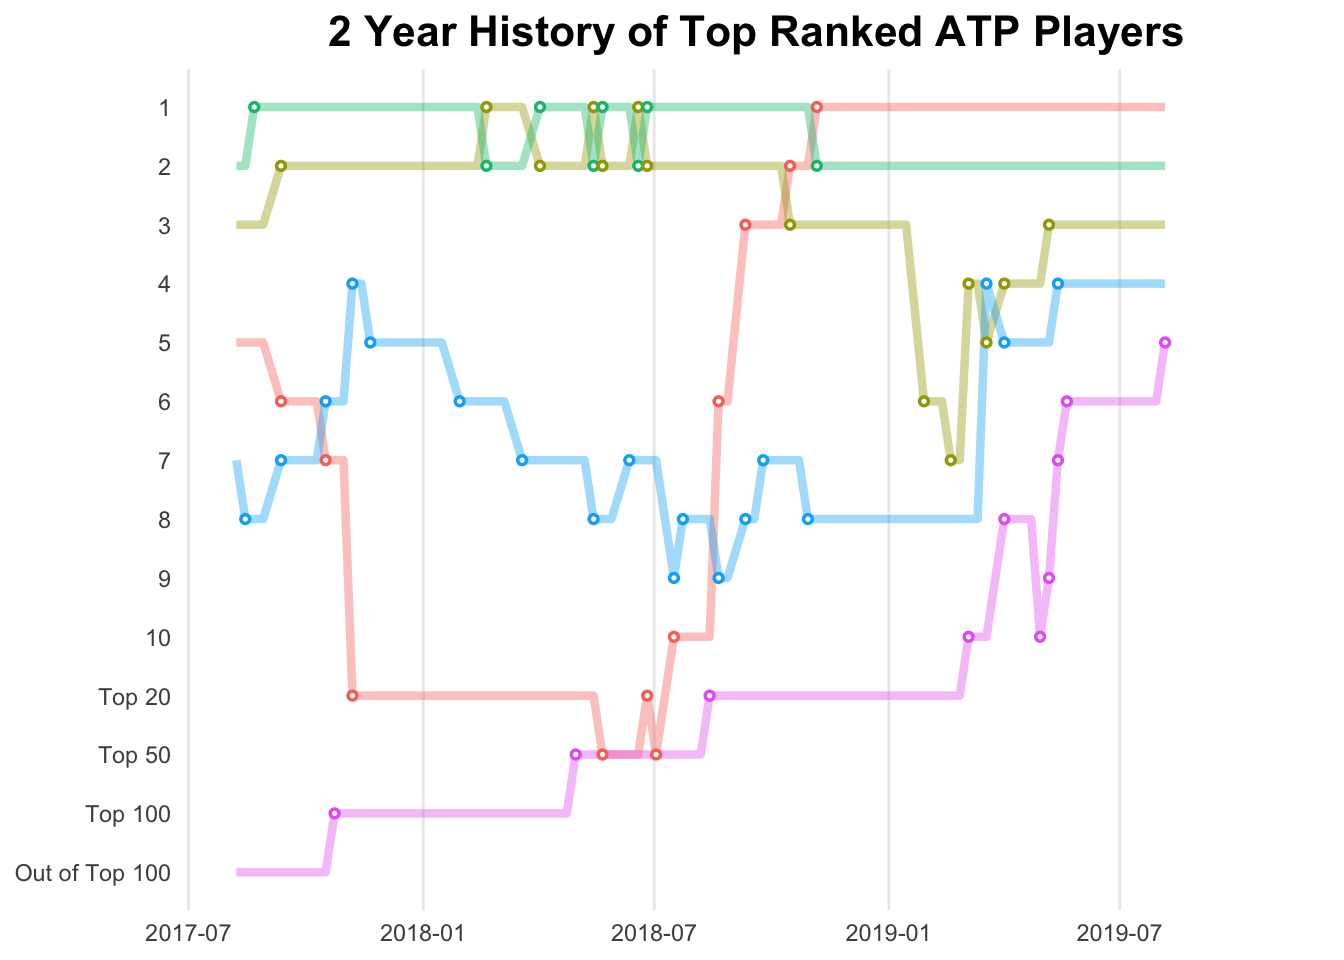
\includegraphics{gggallery_files/figure-latex/unnamed-chunk-57-1.pdf}

Now to add the annotation of the players' names using \emph{geom\_text}.

\begin{Shaded}
\begin{Highlighting}[]
\NormalTok{last_rankings <-}\StringTok{ }\NormalTok{rankings }\OperatorTok\StringTok{ }\KeywordTok{top_n}\NormalTok{(}\DecValTok{5}\NormalTok{, Date) }

\NormalTok{last_rankings}\OperatorTok{$}\NormalTok{nextd <-}\StringTok{ }\NormalTok{next_date}

\NormalTok{atp_plt <-}\StringTok{ }\NormalTok{atp_plt }\OperatorTok{+}\StringTok{ }\KeywordTok{geom_text}\NormalTok{(}\DataTypeTok{data =}\NormalTok{ last_rankings,}
            \KeywordTok{aes}\NormalTok{(}\DataTypeTok{label =}\NormalTok{ Player, }\DataTypeTok{x =}\NormalTok{ nextd,  }\DataTypeTok{colour =}\NormalTok{ Player) , }\DataTypeTok{hjust =} \DecValTok{0}\NormalTok{,}
            \DataTypeTok{fontface =} \StringTok{"bold"}\NormalTok{, }\DataTypeTok{size =} \DecValTok{4}\NormalTok{)}

\NormalTok{atp_plt}
\end{Highlighting}
\end{Shaded}

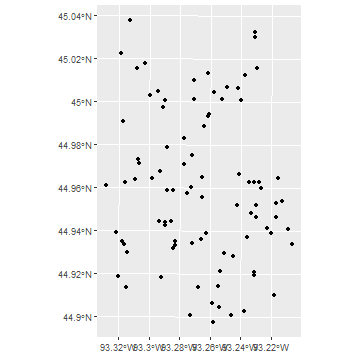
\includegraphics{gggallery_files/figure-latex/unnamed-chunk-58-1.pdf}

The complete code for the plot:

\begin{Shaded}
\begin{Highlighting}[]
\NormalTok{atp_plt <-}\StringTok{ }\KeywordTok{ggplot}\NormalTok{(}\DataTypeTok{data =}\NormalTok{ rankings, }\KeywordTok{aes}\NormalTok{(}\DataTypeTok{x =}\NormalTok{ Date, }\DataTypeTok{y =}\NormalTok{ Ranking, }\DataTypeTok{group =}\NormalTok{ Player)) }\OperatorTok{+}\StringTok{ }
\StringTok{  }\KeywordTok{geom_line}\NormalTok{(}\KeywordTok{aes}\NormalTok{(}\DataTypeTok{color =}\NormalTok{ Player), }\DataTypeTok{alpha =} \FloatTok{0.4}\NormalTok{, }\DataTypeTok{size =} \FloatTok{1.5}\NormalTok{) }\OperatorTok{+}
\StringTok{  }\KeywordTok{scale_y_continuous}\NormalTok{(}\DataTypeTok{breaks =} \KeywordTok{c}\NormalTok{(}\DecValTok{1}\OperatorTok{:}\DecValTok{14}\NormalTok{), }\DataTypeTok{labels =}\NormalTok{ ylabels, }\DataTypeTok{trans =} \StringTok{"reverse"}\NormalTok{) }\OperatorTok{+}\StringTok{ }
\StringTok{  }\KeywordTok{ggtitle}\NormalTok{(}\StringTok{"2 Year History of Top Ranked ATP Players"}\NormalTok{) }\OperatorTok{+}\StringTok{ }
\StringTok{  }\KeywordTok{xlim}\NormalTok{(}\KeywordTok{c}\NormalTok{(begin_date, show_date)) }\OperatorTok{+}
\StringTok{  }\KeywordTok{theme_bw}\NormalTok{() }\OperatorTok{+}\StringTok{ }
\StringTok{  }\KeywordTok{theme}\NormalTok{(}\DataTypeTok{panel.grid.major.y =} \KeywordTok{element_blank}\NormalTok{(), }\DataTypeTok{panel.grid.minor.y =} \KeywordTok{element_blank}\NormalTok{(),}
        \DataTypeTok{panel.grid.minor.x =} \KeywordTok{element_blank}\NormalTok{(), }\DataTypeTok{axis.ticks =} \KeywordTok{element_blank}\NormalTok{(), }
        \DataTypeTok{legend.position =} \StringTok{"none"}\NormalTok{, }\DataTypeTok{panel.border =} \KeywordTok{element_blank}\NormalTok{(),}
        \DataTypeTok{axis.title.x =} \KeywordTok{element_blank}\NormalTok{(), }\DataTypeTok{axis.title.y =} \KeywordTok{element_blank}\NormalTok{(),}
        \DataTypeTok{plot.title =} \KeywordTok{element_text}\NormalTok{(}\DataTypeTok{size =} \DecValTok{16}\NormalTok{, }\DataTypeTok{face =} \StringTok{"bold"}\NormalTok{, }\DataTypeTok{hjust =} \FloatTok{0.5}\NormalTok{)) }\OperatorTok{+}\StringTok{ }\KeywordTok{geom_point}\NormalTok{(}\DataTypeTok{data =}\NormalTok{ changes, }\KeywordTok{aes}\NormalTok{(}\DataTypeTok{x =}\NormalTok{ Date, }\DataTypeTok{y =}\NormalTok{ Ranking, }\DataTypeTok{color =}\NormalTok{ Player)) }\OperatorTok{+}
\StringTok{  }\KeywordTok{geom_point}\NormalTok{(}\DataTypeTok{data =}\NormalTok{ changes, }\DataTypeTok{color =} \StringTok{"#FFFFFF"}\NormalTok{, }\DataTypeTok{size =} \FloatTok{0.25}\NormalTok{) }\OperatorTok{+}\StringTok{ }\KeywordTok{geom_text}\NormalTok{(}\DataTypeTok{data =}\NormalTok{ last_rankings,}
            \KeywordTok{aes}\NormalTok{(}\DataTypeTok{label =}\NormalTok{ Player, }\DataTypeTok{x =}\NormalTok{ nextd,  }\DataTypeTok{colour =}\NormalTok{ Player) , }\DataTypeTok{hjust =} \DecValTok{0}\NormalTok{,}
            \DataTypeTok{fontface =} \StringTok{"bold"}\NormalTok{, }\DataTypeTok{size =} \DecValTok{4}\NormalTok{)}

\NormalTok{atp_plt}
\end{Highlighting}
\end{Shaded}

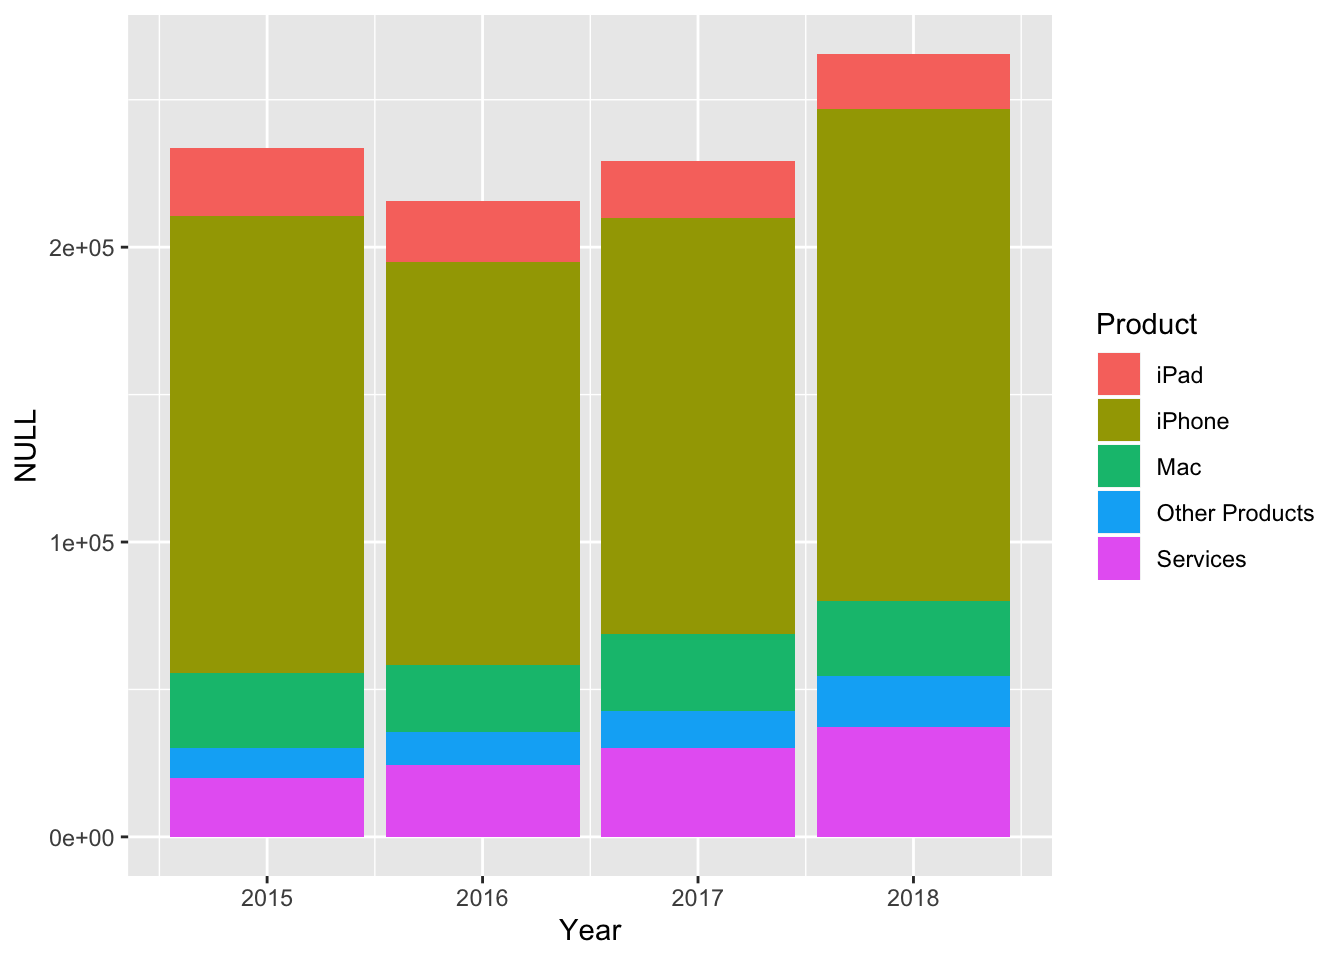
\includegraphics{gggallery_files/figure-latex/unnamed-chunk-59-1.pdf}

\hypertarget{wta}{%
\chapter*{2 Year History of Top-ranked WTA Players}\label{wta}}
\addcontentsline{toc}{chapter}{2 Year History of Top-ranked WTA Players}

\hypertarget{wtadata}{%
\subsubsection*{Data}\label{wtadata}}
\addcontentsline{toc}{subsubsection}{Data}

For this plot, we will use the \emph{wta\_rankings} data frame of the \emph{gcubed} package.

\begin{Shaded}
\begin{Highlighting}[]
\KeywordTok{head}\NormalTok{(wta_rankings)}
\end{Highlighting}
\end{Shaded}

\begin{verbatim}
## # A tibble: 6 x 6
##   Month   Day  Year Singles Player   Date               
##   <dbl> <dbl> <dbl>   <int> <chr>    <dttm>             
## 1     8     7  2017      58 Barty    2017-08-07 12:00:00
## 2     8     7  2017      50 Osaka    2017-08-07 12:00:00
## 3     8     7  2017       1 Pliskova 2017-08-07 12:00:00
## 4     8     7  2017       2 Halep    2017-08-07 12:00:00
## 5     8     7  2017      27 Bertens  2017-08-07 12:00:00
## 6     8    14  2017      48 Barty    2017-08-14 12:00:00
\end{verbatim}

First, create a new variable, \emph{Ranking} that preserves the rankings when the player is in the top 10. When the player is not in the top 10, the new variable is set to: 11 if the player is in the top 20; 12 if the player is ranked between 21 and 50 (inclusive); 13 if the player is ranked between 51 and 100 (inclusive); 14 if the player is ranked lower than 100.

Also, we create a variable \emph{Change} to be used later to identify the points in time when the players' rankings changed.

\begin{Shaded}
\begin{Highlighting}[]
\NormalTok{rankings <-}\StringTok{ }\KeywordTok{mutate}\NormalTok{(wta_rankings, }\DataTypeTok{Ranking =} \KeywordTok{ifelse}\NormalTok{(Singles }\OperatorTok{>}\StringTok{ }\DecValTok{100}\NormalTok{, }\DecValTok{14}\NormalTok{, }
                          \KeywordTok{ifelse}\NormalTok{(Singles }\OperatorTok{>}\StringTok{ }\DecValTok{50}\NormalTok{, }\DecValTok{13}\NormalTok{, }
                                 \KeywordTok{ifelse}\NormalTok{(Singles }\OperatorTok{>}\StringTok{ }\DecValTok{20}\NormalTok{, }\DecValTok{12}\NormalTok{, }
                                        \KeywordTok{ifelse}\NormalTok{(Singles }\OperatorTok{>}\StringTok{ }\DecValTok{10}\NormalTok{, }\DecValTok{11}\NormalTok{, Singles))))) }\OperatorTok
\StringTok{  }\KeywordTok{group_by}\NormalTok{(Player) }\OperatorTok\StringTok{ }\KeywordTok{mutate}\NormalTok{(}\DataTypeTok{Change =} \KeywordTok{c}\NormalTok{(}\DecValTok{0}\NormalTok{,}\KeywordTok{diff}\NormalTok{(Ranking))) }\OperatorTok\StringTok{ }\KeywordTok{ungroup}\NormalTok{()}
\end{Highlighting}
\end{Shaded}

\hypertarget{wtacode}{%
\subsubsection*{Code for plot}\label{wtacode}}
\addcontentsline{toc}{subsubsection}{Code for plot}

\begin{Shaded}
\begin{Highlighting}[]
\NormalTok{ylabels <-}\StringTok{ }\KeywordTok{c}\NormalTok{(}\DecValTok{1}\OperatorTok{:}\DecValTok{10}\NormalTok{, }\StringTok{"Top 20"}\NormalTok{, }\StringTok{"Top 50"}\NormalTok{, }\StringTok{"Top 100"}\NormalTok{, }\StringTok{"Out of Top 100"}\NormalTok{)}


\NormalTok{show_date <-}\StringTok{ }\KeywordTok{ISOdate}\NormalTok{(}\DecValTok{2019}\NormalTok{, }\DecValTok{11}\NormalTok{,}\DecValTok{1}\NormalTok{)}
\NormalTok{begin_date <-}\StringTok{ }\KeywordTok{ISOdate}\NormalTok{(}\DecValTok{2017}\NormalTok{, }\DecValTok{8}\NormalTok{, }\DecValTok{7}\NormalTok{)}
\NormalTok{next_date <-}\StringTok{ }\KeywordTok{ISOdate}\NormalTok{(}\DecValTok{2019}\NormalTok{, }\DecValTok{8}\NormalTok{, }\DecValTok{15}\NormalTok{)}


\NormalTok{wta_plt <-}\StringTok{ }\KeywordTok{ggplot}\NormalTok{(}\DataTypeTok{data =}\NormalTok{ rankings, }\KeywordTok{aes}\NormalTok{(}\DataTypeTok{x =}\NormalTok{ Date, }\DataTypeTok{y =}\NormalTok{ Ranking, }\DataTypeTok{group =}\NormalTok{ Player)) }\OperatorTok{+}\StringTok{ }
\StringTok{  }\KeywordTok{geom_line}\NormalTok{(}\KeywordTok{aes}\NormalTok{(}\DataTypeTok{color =}\NormalTok{ Player), }\DataTypeTok{alpha =} \FloatTok{0.4}\NormalTok{, }\DataTypeTok{size =} \FloatTok{1.5}\NormalTok{) }\OperatorTok{+}
\StringTok{  }\KeywordTok{scale_y_continuous}\NormalTok{(}\DataTypeTok{breaks =} \KeywordTok{c}\NormalTok{(}\DecValTok{1}\OperatorTok{:}\DecValTok{14}\NormalTok{), }\DataTypeTok{labels =}\NormalTok{ ylabels, }\DataTypeTok{trans =} \StringTok{"reverse"}\NormalTok{) }\OperatorTok{+}\StringTok{ }
\StringTok{  }\KeywordTok{ggtitle}\NormalTok{(}\StringTok{"2 Year History of Top Ranked WTA Players"}\NormalTok{) }\OperatorTok{+}\StringTok{ }
\StringTok{  }\KeywordTok{xlim}\NormalTok{(}\KeywordTok{c}\NormalTok{(begin_date, show_date)) }\OperatorTok{+}
\StringTok{  }\KeywordTok{theme_bw}\NormalTok{() }

\NormalTok{wta_plt}
\end{Highlighting}
\end{Shaded}

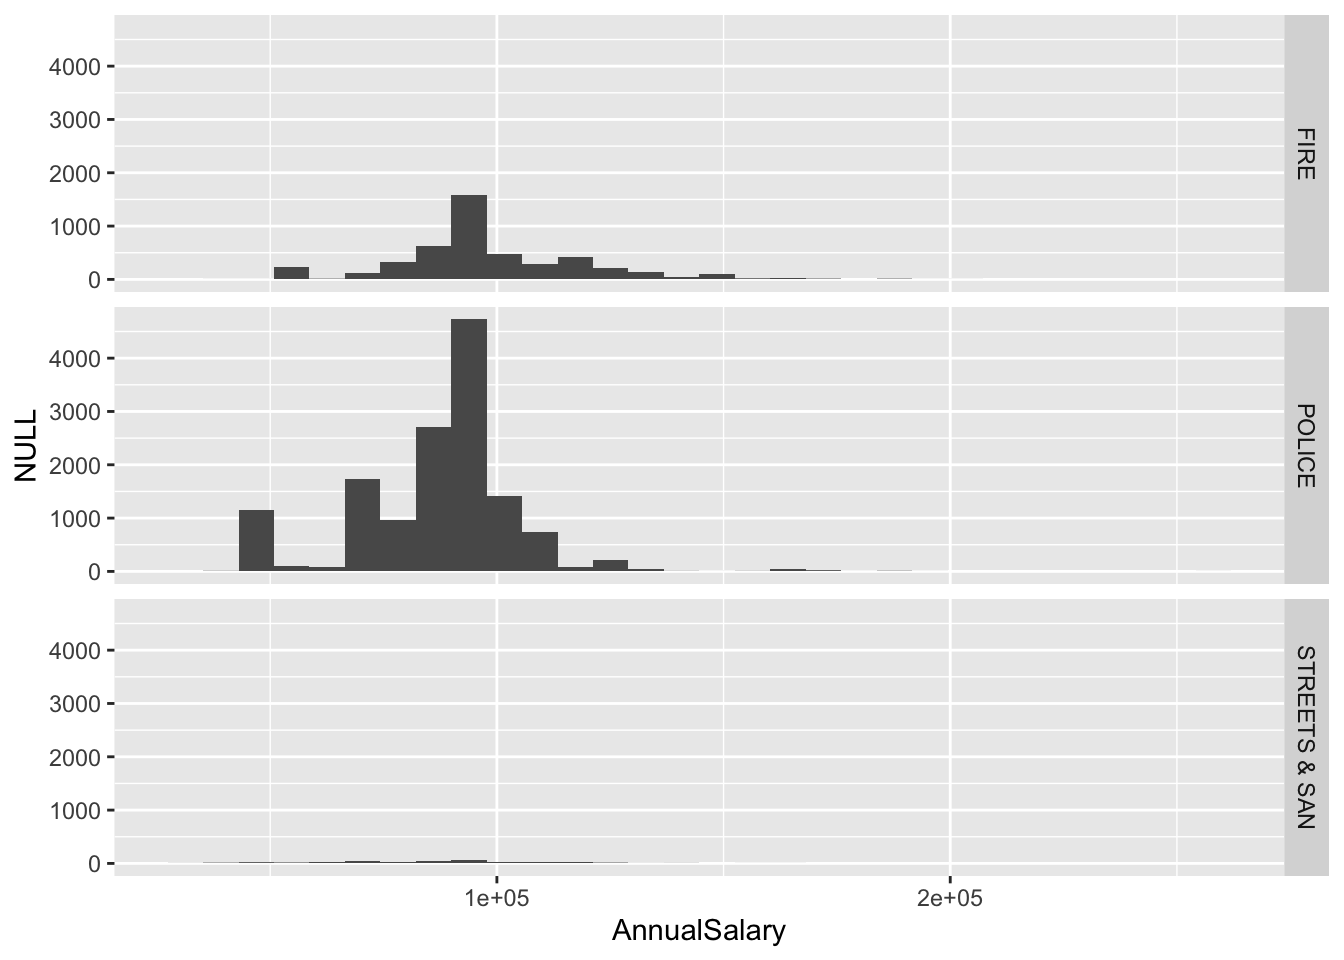
\includegraphics{gggallery_files/figure-latex/unnamed-chunk-63-1.pdf}

Next, we can change the overall look of the plot using the \emph{theme} function to change several
details of the graph.

\begin{Shaded}
\begin{Highlighting}[]
\NormalTok{wta_plt <-}\StringTok{ }\NormalTok{wta_plt }\OperatorTok{+}\StringTok{ }
\StringTok{  }\KeywordTok{theme}\NormalTok{(}\DataTypeTok{panel.grid.major.y =} \KeywordTok{element_blank}\NormalTok{(), }\DataTypeTok{panel.grid.minor.y =} \KeywordTok{element_blank}\NormalTok{(),}
        \DataTypeTok{panel.grid.minor.x =} \KeywordTok{element_blank}\NormalTok{(), }\DataTypeTok{axis.ticks =} \KeywordTok{element_blank}\NormalTok{(), }
        \DataTypeTok{legend.position =} \StringTok{"none"}\NormalTok{, }\DataTypeTok{panel.border =} \KeywordTok{element_blank}\NormalTok{(),}
        \DataTypeTok{axis.title.x =} \KeywordTok{element_blank}\NormalTok{(), }\DataTypeTok{axis.title.y =} \KeywordTok{element_blank}\NormalTok{(),}
        \DataTypeTok{plot.title =} \KeywordTok{element_text}\NormalTok{(}\DataTypeTok{size =} \DecValTok{16}\NormalTok{, }\DataTypeTok{face =} \StringTok{"bold"}\NormalTok{, }\DataTypeTok{hjust =} \FloatTok{0.5}\NormalTok{)) }

\NormalTok{wta_plt}
\end{Highlighting}
\end{Shaded}

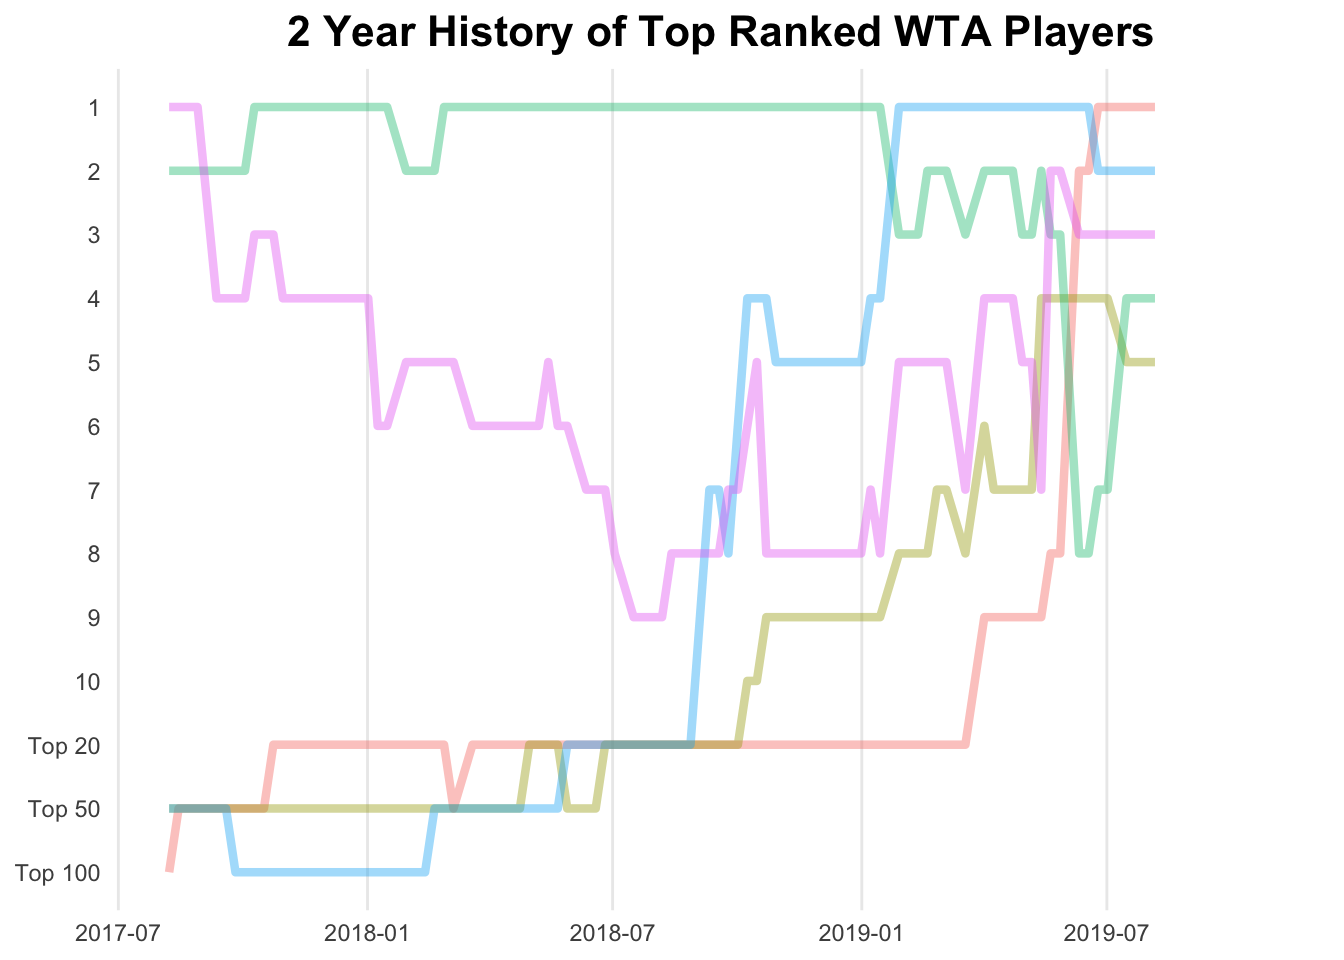
\includegraphics{gggallery_files/figure-latex/unnamed-chunk-64-1.pdf}

Adding some points to signify the times at which the players' rankings changed using \emph{geom\_point}.
We are going to use two \emph{geom\_point} geometries to create a smaller white circle inside the coloured larger circles.

\begin{Shaded}
\begin{Highlighting}[]
\NormalTok{changes <-}\StringTok{ }\KeywordTok{filter}\NormalTok{(rankings, Change }\OperatorTok{!=}\StringTok{ }\DecValTok{0}\NormalTok{)}


\NormalTok{wta_plt <-}\StringTok{ }\NormalTok{wta_plt }\OperatorTok{+}\StringTok{ }\KeywordTok{geom_point}\NormalTok{(}\DataTypeTok{data =}\NormalTok{ changes, }\KeywordTok{aes}\NormalTok{(}\DataTypeTok{x =}\NormalTok{ Date, }\DataTypeTok{y =}\NormalTok{ Ranking, }\DataTypeTok{color =}\NormalTok{ Player)) }\OperatorTok{+}
\StringTok{  }\KeywordTok{geom_point}\NormalTok{(}\DataTypeTok{data =}\NormalTok{ changes, }\DataTypeTok{color =} \StringTok{"#FFFFFF"}\NormalTok{, }\DataTypeTok{size =} \FloatTok{0.25}\NormalTok{) }

\NormalTok{wta_plt}
\end{Highlighting}
\end{Shaded}

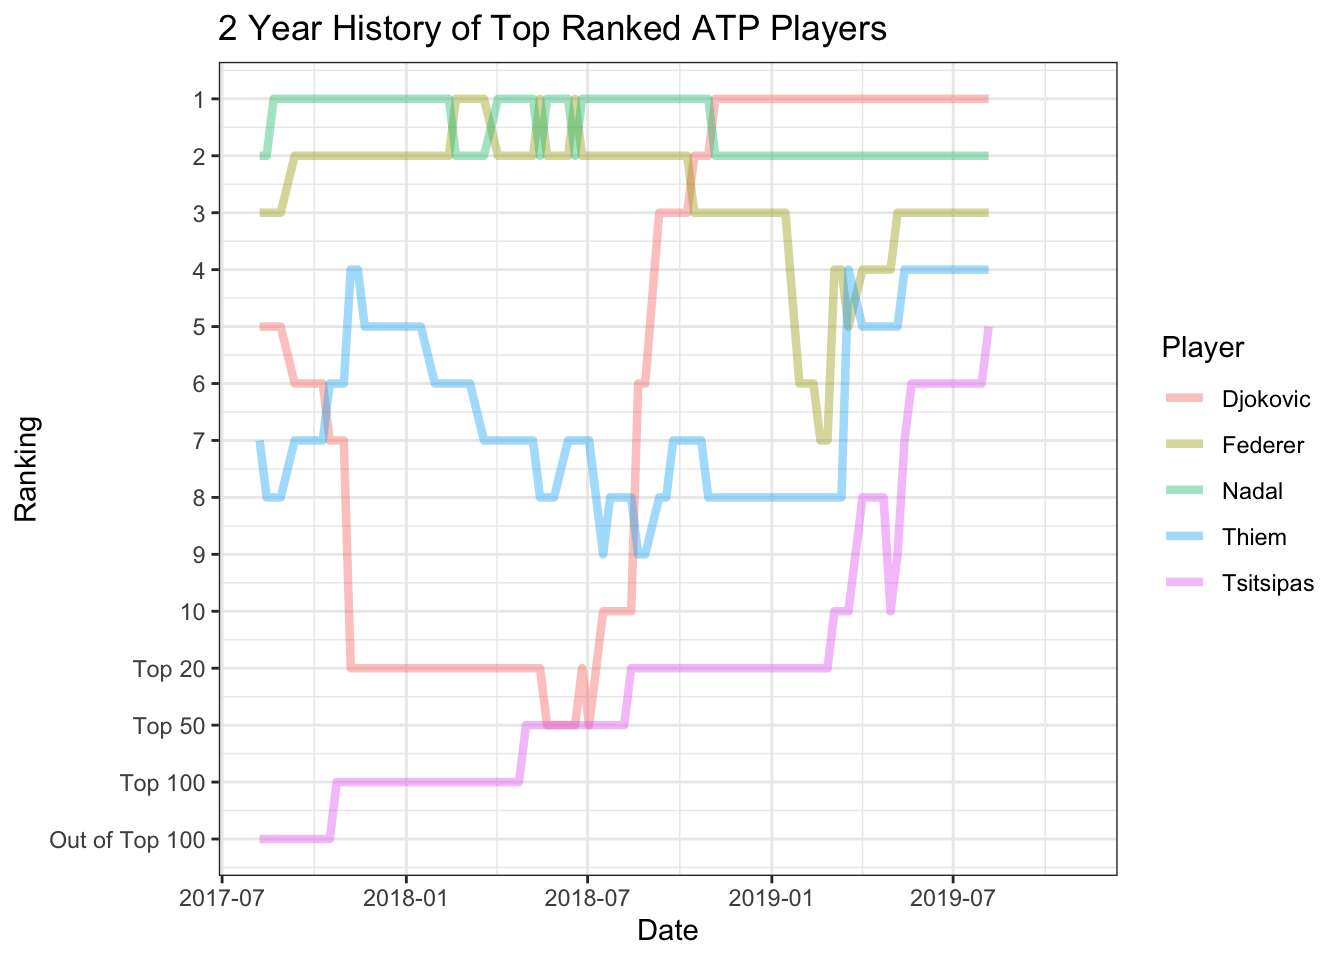
\includegraphics{gggallery_files/figure-latex/unnamed-chunk-65-1.pdf}

Now to add the annotation of the players' names using \emph{geom\_text}.

\begin{Shaded}
\begin{Highlighting}[]
\NormalTok{last_rankings <-}\StringTok{ }\NormalTok{rankings }\OperatorTok\StringTok{ }\KeywordTok{top_n}\NormalTok{(}\DecValTok{5}\NormalTok{, Date) }

\NormalTok{last_rankings}\OperatorTok{$}\NormalTok{nextd <-}\StringTok{ }\NormalTok{next_date}

\NormalTok{wta_plt <-}\StringTok{ }\NormalTok{wta_plt }\OperatorTok{+}\StringTok{ }\KeywordTok{geom_text}\NormalTok{(}\DataTypeTok{data =}\NormalTok{ last_rankings,}
            \KeywordTok{aes}\NormalTok{(}\DataTypeTok{label =}\NormalTok{ Player, }\DataTypeTok{x =}\NormalTok{ nextd,  }\DataTypeTok{colour =}\NormalTok{ Player) , }\DataTypeTok{hjust =} \DecValTok{0}\NormalTok{,}
            \DataTypeTok{fontface =} \StringTok{"bold"}\NormalTok{, }\DataTypeTok{size =} \DecValTok{4}\NormalTok{)}

\NormalTok{wta_plt}
\end{Highlighting}
\end{Shaded}

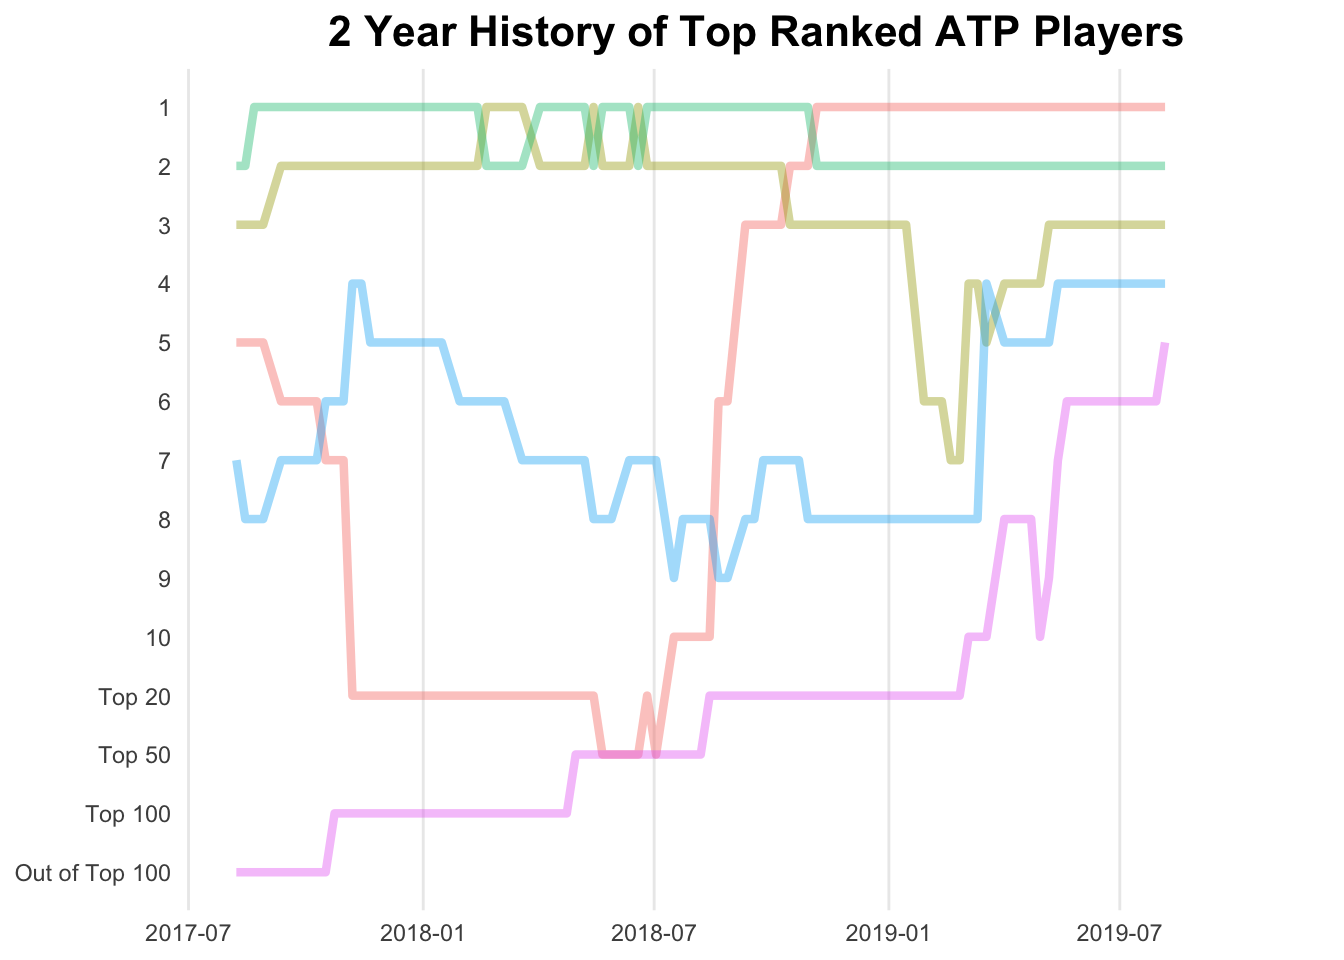
\includegraphics{gggallery_files/figure-latex/unnamed-chunk-66-1.pdf}

The complete code for the plot:

\begin{Shaded}
\begin{Highlighting}[]
\NormalTok{wta_plt <-}\StringTok{ }\KeywordTok{ggplot}\NormalTok{(}\DataTypeTok{data =}\NormalTok{ rankings, }\KeywordTok{aes}\NormalTok{(}\DataTypeTok{x =}\NormalTok{ Date, }\DataTypeTok{y =}\NormalTok{ Ranking, }\DataTypeTok{group =}\NormalTok{ Player)) }\OperatorTok{+}\StringTok{ }
\StringTok{  }\KeywordTok{geom_line}\NormalTok{(}\KeywordTok{aes}\NormalTok{(}\DataTypeTok{color =}\NormalTok{ Player), }\DataTypeTok{alpha =} \FloatTok{0.4}\NormalTok{, }\DataTypeTok{size =} \FloatTok{1.5}\NormalTok{) }\OperatorTok{+}
\StringTok{  }\KeywordTok{scale_y_continuous}\NormalTok{(}\DataTypeTok{breaks =} \KeywordTok{c}\NormalTok{(}\DecValTok{1}\OperatorTok{:}\DecValTok{14}\NormalTok{), }\DataTypeTok{labels =}\NormalTok{ ylabels, }\DataTypeTok{trans =} \StringTok{"reverse"}\NormalTok{) }\OperatorTok{+}\StringTok{ }
\StringTok{  }\KeywordTok{ggtitle}\NormalTok{(}\StringTok{"2 Year History of Top Ranked WTA Players"}\NormalTok{) }\OperatorTok{+}\StringTok{ }
\StringTok{  }\KeywordTok{xlim}\NormalTok{(}\KeywordTok{c}\NormalTok{(begin_date, show_date)) }\OperatorTok{+}
\StringTok{  }\KeywordTok{theme_bw}\NormalTok{() }\OperatorTok{+}\StringTok{ }
\StringTok{  }\KeywordTok{theme}\NormalTok{(}\DataTypeTok{panel.grid.major.y =} \KeywordTok{element_blank}\NormalTok{(), }\DataTypeTok{panel.grid.minor.y =} \KeywordTok{element_blank}\NormalTok{(),}
        \DataTypeTok{panel.grid.minor.x =} \KeywordTok{element_blank}\NormalTok{(), }\DataTypeTok{axis.ticks =} \KeywordTok{element_blank}\NormalTok{(), }
        \DataTypeTok{legend.position =} \StringTok{"none"}\NormalTok{, }\DataTypeTok{panel.border =} \KeywordTok{element_blank}\NormalTok{(),}
        \DataTypeTok{axis.title.x =} \KeywordTok{element_blank}\NormalTok{(), }\DataTypeTok{axis.title.y =} \KeywordTok{element_blank}\NormalTok{(),}
        \DataTypeTok{plot.title =} \KeywordTok{element_text}\NormalTok{(}\DataTypeTok{size =} \DecValTok{16}\NormalTok{, }\DataTypeTok{face =} \StringTok{"bold"}\NormalTok{, }\DataTypeTok{hjust =} \FloatTok{0.5}\NormalTok{)) }\OperatorTok{+}\StringTok{ }\KeywordTok{geom_point}\NormalTok{(}\DataTypeTok{data =}\NormalTok{ changes, }\KeywordTok{aes}\NormalTok{(}\DataTypeTok{x =}\NormalTok{ Date, }\DataTypeTok{y =}\NormalTok{ Ranking, }\DataTypeTok{color =}\NormalTok{ Player)) }\OperatorTok{+}
\StringTok{  }\KeywordTok{geom_point}\NormalTok{(}\DataTypeTok{data =}\NormalTok{ changes, }\DataTypeTok{color =} \StringTok{"#FFFFFF"}\NormalTok{, }\DataTypeTok{size =} \FloatTok{0.25}\NormalTok{) }\OperatorTok{+}\StringTok{ }\KeywordTok{geom_text}\NormalTok{(}\DataTypeTok{data =}\NormalTok{ last_rankings,}
            \KeywordTok{aes}\NormalTok{(}\DataTypeTok{label =}\NormalTok{ Player, }\DataTypeTok{x =}\NormalTok{ nextd,  }\DataTypeTok{colour =}\NormalTok{ Player) , }\DataTypeTok{hjust =} \DecValTok{0}\NormalTok{,}
            \DataTypeTok{fontface =} \StringTok{"bold"}\NormalTok{, }\DataTypeTok{size =} \DecValTok{4}\NormalTok{)}

\NormalTok{wta_plt}
\end{Highlighting}
\end{Shaded}

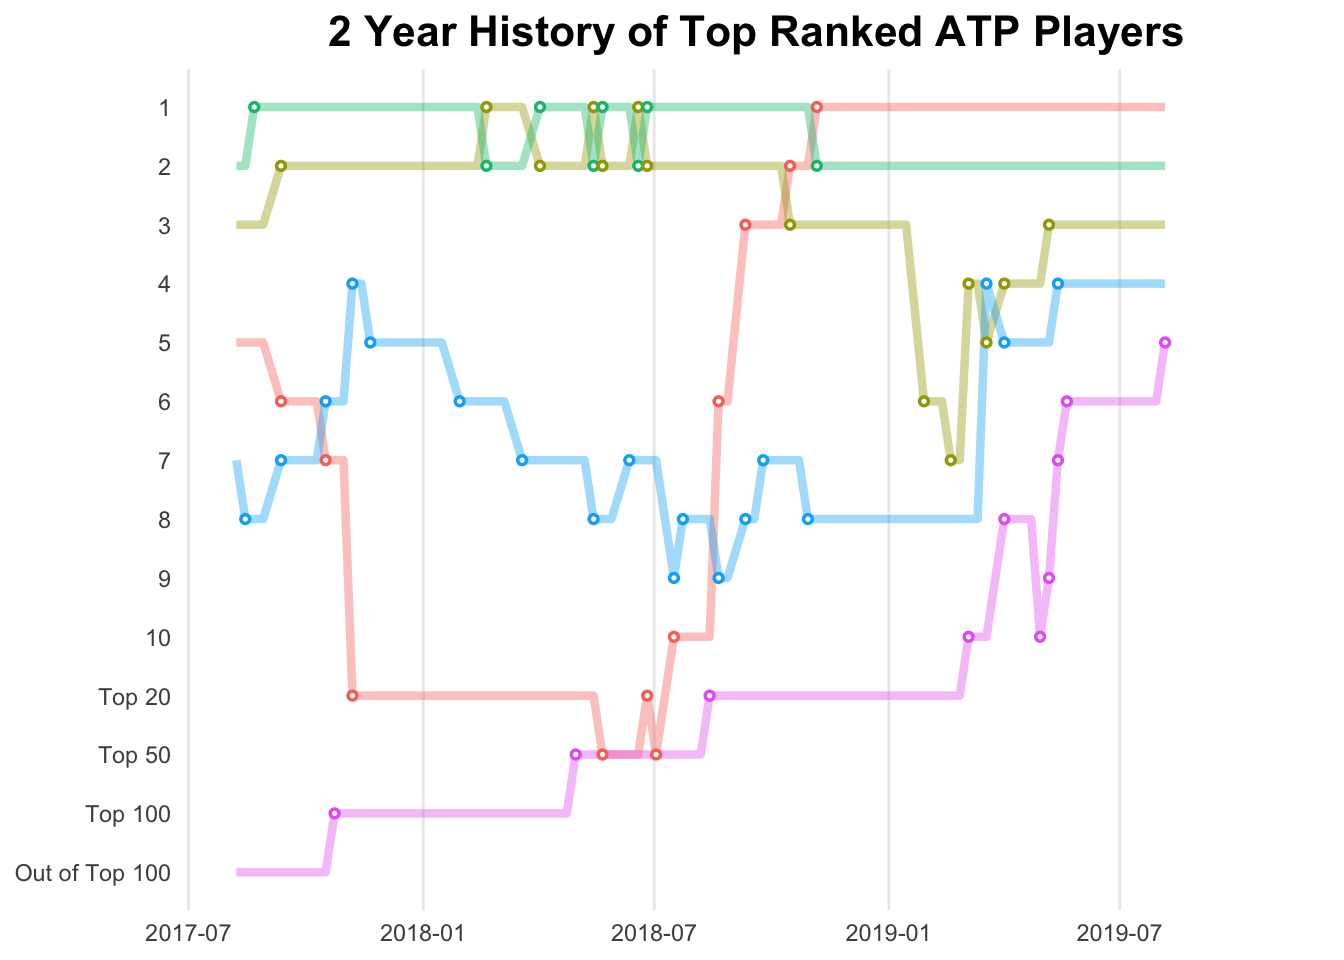
\includegraphics{gggallery_files/figure-latex/unnamed-chunk-67-1.pdf}

\hypertarget{sp}{%
\chapter*{S\&P 500 daily returns in 2018}\label{sp}}
\addcontentsline{toc}{chapter}{S\&P 500 daily returns in 2018}

\hypertarget{spdata}{%
\paragraph{Data}\label{spdata}}
\addcontentsline{toc}{paragraph}{Data}

This plot uses the \emph{sp500} data frame of the \emph{gcubed} package.

\begin{Shaded}
\begin{Highlighting}[]
\KeywordTok{tail}\NormalTok{(sp500)}
\end{Highlighting}
\end{Shaded}

\begin{verbatim}
## # A tibble: 6 x 7
##   Month   Day  Year  Open Close PrevClose daily_return
##   <int> <int> <int> <dbl> <dbl>     <dbl>        <dbl>
## 1    12    21  2018 2465. 2417.     2467.       -2.06 
## 2    12    24  2018 2401. 2351.     2417.       -2.71 
## 3    12    26  2018 2363. 2468.     2351.        4.96 
## 4    12    27  2018 2442. 2489.     2468.        0.856
## 5    12    28  2018 2499. 2486.     2489.       -0.124
## 6    12    31  2018 2499. 2507.     2486.        0.849
\end{verbatim}

First, we will restrict the data to only those entries from the year 2018. Then we will create a new column, \emph{updown} that will simply say whether or not each day's return represented a gain or a loss. This will be used later to colour the bars of the plot.

\hypertarget{spcode}{%
\subsubsection*{Code for plot}\label{spcode}}
\addcontentsline{toc}{subsubsection}{Code for plot}

We will use the \emph{geom\_bar} geometry to create this plot. The \emph{fill} aesthetic\_ will be used to colour the bars appropriately for positive and negative daily returns.

\begin{Shaded}
\begin{Highlighting}[]
\KeywordTok{library}\NormalTok{(ggplot2)}

\NormalTok{sp18_plt <-}\StringTok{ }\KeywordTok{ggplot}\NormalTok{(}\DataTypeTok{data =}\NormalTok{ sp18, }\KeywordTok{aes}\NormalTok{(}\DataTypeTok{x =}\NormalTok{ Date, }\DataTypeTok{y =}\NormalTok{ daily_return, }\DataTypeTok{fill =}\NormalTok{ updown )) }\OperatorTok{+}
\StringTok{  }\KeywordTok{geom_bar}\NormalTok{(}\DataTypeTok{stat =} \StringTok{"identity"}\NormalTok{) }\OperatorTok{+}
\StringTok{  }\KeywordTok{ylab}\NormalTok{(}\StringTok{"Daily Returns (% of Prev Close)"}\NormalTok{)}\OperatorTok{+}
\StringTok{  }\KeywordTok{guides}\NormalTok{(}\DataTypeTok{fill =} \KeywordTok{guide_legend}\NormalTok{(}\DataTypeTok{override.aes=} \KeywordTok{list}\NormalTok{(}\DataTypeTok{alpha =} \FloatTok{0.2}\NormalTok{))) }\OperatorTok{+}
\StringTok{  }\KeywordTok{ggtitle}\NormalTok{(}\StringTok{"S&P 500 Daily Returns (2018) "}\NormalTok{) }\OperatorTok{+}
\StringTok{  }\KeywordTok{theme}\NormalTok{(}\DataTypeTok{plot.title =} \KeywordTok{element_text}\NormalTok{(}\DataTypeTok{size =} \DecValTok{16}\NormalTok{, }\DataTypeTok{face =} \StringTok{"bold"}\NormalTok{, }\DataTypeTok{hjust =} \FloatTok{0.5}\NormalTok{), }
        \DataTypeTok{panel.background =} \KeywordTok{element_blank}\NormalTok{(),}
        \DataTypeTok{axis.title.x=}\KeywordTok{element_blank}\NormalTok{(),}
        \DataTypeTok{legend.position =} \StringTok{"none"}\NormalTok{) }\OperatorTok{+}\StringTok{ }
\StringTok{  }\KeywordTok{scale_fill_manual}\NormalTok{(}\DataTypeTok{values =} \KeywordTok{c}\NormalTok{(}\StringTok{"blue"}\NormalTok{, }\StringTok{"red"}\NormalTok{))}

\NormalTok{sp18_plt}
\end{Highlighting}
\end{Shaded}

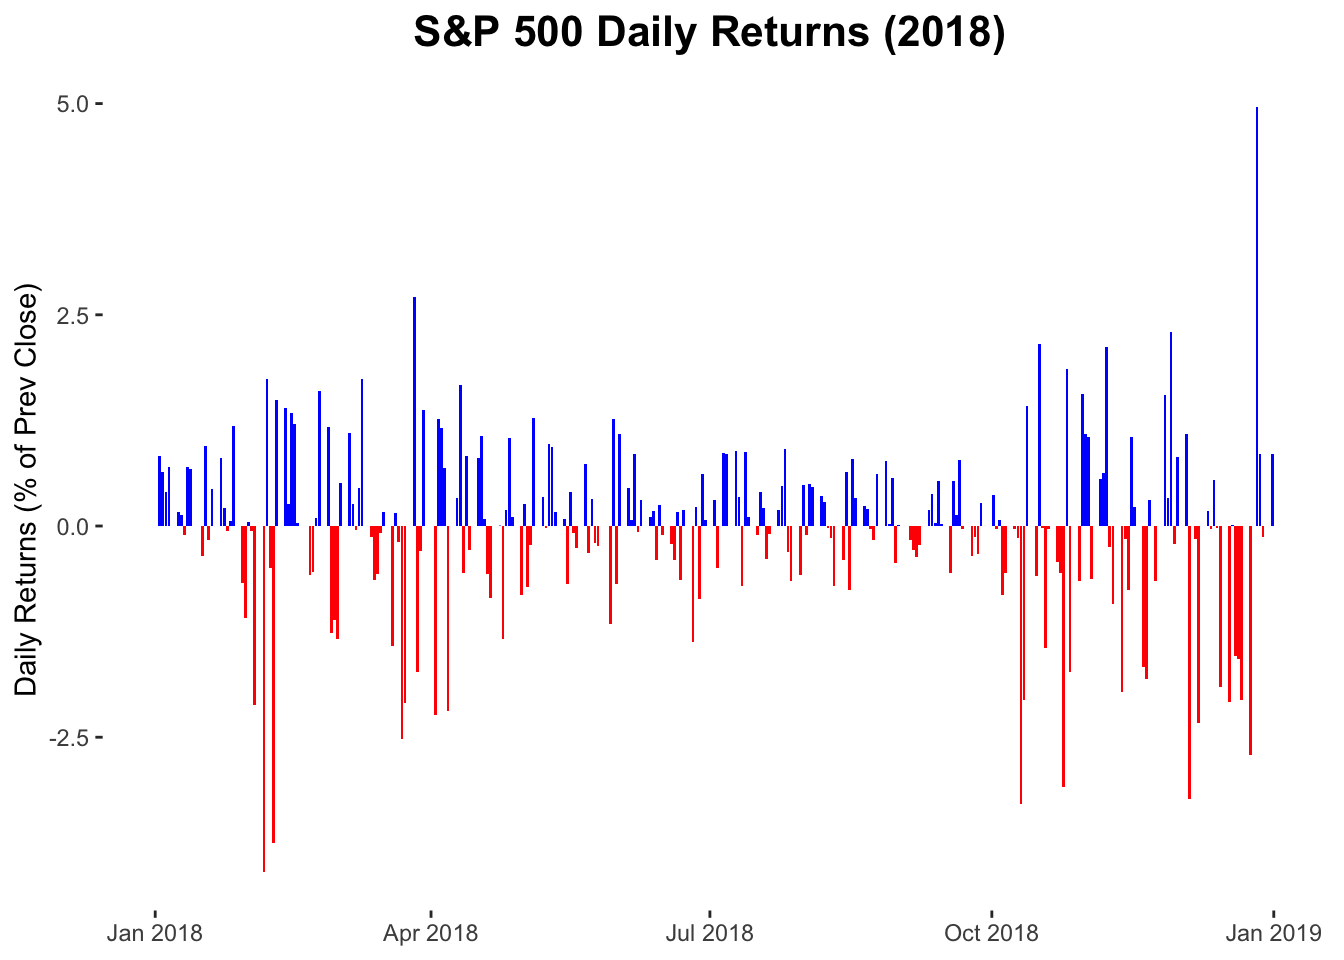
\includegraphics{gggallery_files/figure-latex/unnamed-chunk-72-1.pdf}

\hypertarget{spfour}{%
\chapter*{S\&P 500 daily returns 2015 - 2018}\label{spfour}}
\addcontentsline{toc}{chapter}{S\&P 500 daily returns 2015 - 2018}

\hypertarget{spfourdata}{%
\paragraph{Data}\label{spfourdata}}
\addcontentsline{toc}{paragraph}{Data}

This plot uses the \emph{sp500} data frame of the \emph{gcubed} package. Rows 250, 500, 750 and 1000 of the data frame are shown below.

\begin{Shaded}
\begin{Highlighting}[]
\NormalTok{sp500[}\KeywordTok{c}\NormalTok{(}\DecValTok{250}\NormalTok{,}\DecValTok{500}\NormalTok{,}\DecValTok{750}\NormalTok{,}\DecValTok{1000}\NormalTok{),]}
\end{Highlighting}
\end{Shaded}

\begin{verbatim}
## # A tibble: 4 x 7
##   Month   Day  Year  Open Close PrevClose daily_return
##   <int> <int> <int> <dbl> <dbl>     <dbl>        <dbl>
## 1    12    29  2015 2061. 2078.     2056.        1.06 
## 2    12    23  2016 2260. 2264.     2261.        0.125
## 3    12    21  2017 2683. 2685.     2679.        0.199
## 4    12    20  2018 2497. 2467.     2507.       -1.58
\end{verbatim}

First, we will restrict the data to only those entries from the year 2018. Then we will create a new column, \emph{updown} that will simply say whether or not each day's return represented a gain or a loss. This will be used later to colour the bars of the plot.

\begin{verbatim}
## # A tibble: 4 x 8
##   Month   Day  Year  Open Close PrevClose daily_return MonthDay
##   <int> <int> <int> <dbl> <dbl>     <dbl>        <dbl> <chr>   
## 1    12    29  2015 2061. 2078.     2056.        1.06  12-29   
## 2    12    23  2016 2260. 2264.     2261.        0.125 12-23   
## 3    12    21  2017 2683. 2685.     2679.        0.199 12-21   
## 4     5    27  2015 2105. 2123.     2104.        0.916 05-27
\end{verbatim}

\hypertarget{spfourcode}{%
\subsubsection*{Code for plot}\label{spfourcode}}
\addcontentsline{toc}{subsubsection}{Code for plot}

We will use the \emph{geom\_bar} geometry to create this plot. The \emph{fill} aesthetic\_ will be used to colour the bars appropriately for positive and negative daily returns.

\begin{Shaded}
\begin{Highlighting}[]
\NormalTok{sp_plt <-}\StringTok{ }\KeywordTok{ggplot}\NormalTok{(}\DataTypeTok{data =}\NormalTok{ df, }\KeywordTok{aes}\NormalTok{(}\DataTypeTok{x =}\NormalTok{ MonthDay, }\DataTypeTok{y =}\NormalTok{ daily_return)) }\OperatorTok{+}
\StringTok{  }\KeywordTok{geom_bar}\NormalTok{(}\DataTypeTok{stat =} \StringTok{"identity"}\NormalTok{) }\OperatorTok{+}
\StringTok{  }\KeywordTok{facet_wrap}\NormalTok{(}\OperatorTok{~}\NormalTok{Year) }\OperatorTok{+}\StringTok{ }
\StringTok{  }\KeywordTok{ylab}\NormalTok{(}\StringTok{"Daily Returns (% of Prev Close)"}\NormalTok{) }\OperatorTok{+}
\StringTok{  }\KeywordTok{ggtitle}\NormalTok{(}\StringTok{"S&P 500 Daily Returns (2015 - 2018)"}\NormalTok{)}
  

\NormalTok{sp_plt}
\end{Highlighting}
\end{Shaded}

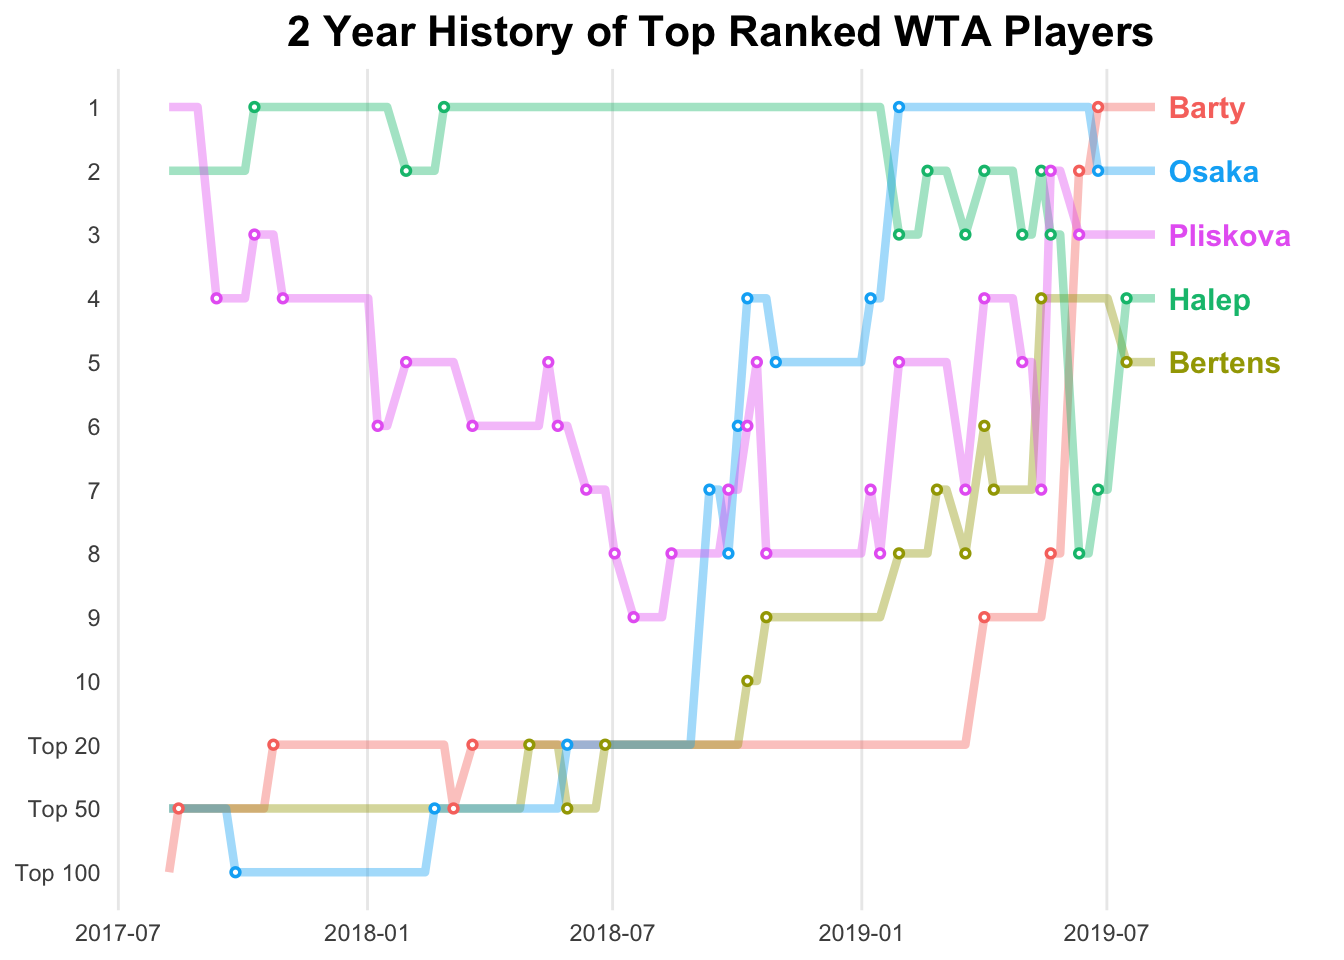
\includegraphics{gggallery_files/figure-latex/unnamed-chunk-77-1.pdf}

At present the x-axis labels are from a categorical variable, \emph{MonthDay}. The hundreds of overlapping values being displayed can be removed to de-clutter the lower portion of the plot.

\begin{Shaded}
\begin{Highlighting}[]
\NormalTok{sp_plt <-}\StringTok{ }\NormalTok{sp_plt }\OperatorTok{+}\StringTok{ }
\StringTok{  }\KeywordTok{theme}\NormalTok{(}\DataTypeTok{plot.title =} \KeywordTok{element_text}\NormalTok{(}\DataTypeTok{size =} \DecValTok{16}\NormalTok{, }\DataTypeTok{face =} \StringTok{"bold"}\NormalTok{, }\DataTypeTok{hjust =} \FloatTok{0.5}\NormalTok{), }
        \DataTypeTok{panel.background =} \KeywordTok{element_blank}\NormalTok{(), }\DataTypeTok{axis.title.x=}\KeywordTok{element_blank}\NormalTok{(), }
        \DataTypeTok{axis.text.x =}  \KeywordTok{element_blank}\NormalTok{(), }\DataTypeTok{axis.ticks.x =} \KeywordTok{element_blank}\NormalTok{()) }

\NormalTok{sp_plt}
\end{Highlighting}
\end{Shaded}

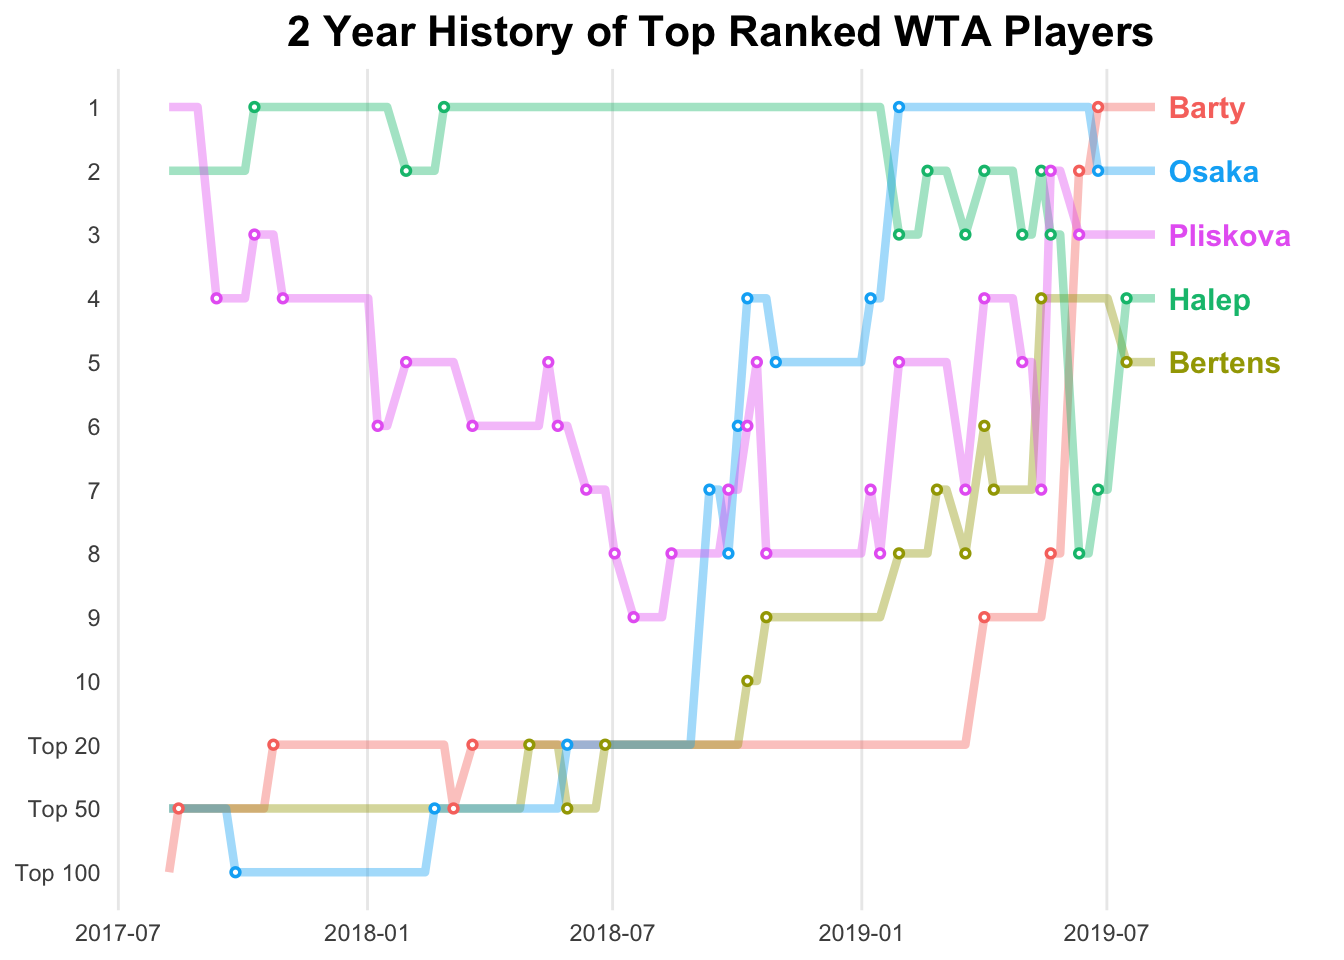
\includegraphics{gggallery_files/figure-latex/unnamed-chunk-78-1.pdf}

To add bands representing 95th and 99th percentile moves, first we use determine what the 95th and 99th percentile moves are.

\begin{Shaded}
\begin{Highlighting}[]
\NormalTok{df}\OperatorTok{$}\NormalTok{abs_return <-}\StringTok{ }\KeywordTok{abs}\NormalTok{(df}\OperatorTok{$}\NormalTok{daily_return)}
\KeywordTok{head}\NormalTok{(df)}
\end{Highlighting}
\end{Shaded}

\begin{verbatim}
## # A tibble: 6 x 9
##   Month   Day  Year  Open Close PrevClose daily_return MonthDay abs_return
##   <int> <int> <int> <dbl> <dbl>     <dbl>        <dbl> <chr>         <dbl>
## 1     1     2  2015 2059. 2058.     2059.      -0.0340 01-02        0.0340
## 2     1     5  2015 2054. 2021.     2058.      -1.83   01-05        1.83  
## 3     1     6  2015 2022. 2003.     2021.      -0.889  01-06        0.889 
## 4     1     7  2015 2006. 2026.     2003.       1.16   01-07        1.16  
## 5     1     8  2015 2031. 2062.     2026.       1.79   01-08        1.79  
## 6     1     9  2015 2063. 2045.     2062.      -0.840  01-09        0.840
\end{verbatim}

\begin{Shaded}
\begin{Highlighting}[]
\NormalTok{pct95 <-}\StringTok{ }\KeywordTok{quantile}\NormalTok{(df}\OperatorTok{$}\NormalTok{abs_return, }\FloatTok{.95}\NormalTok{)}
\NormalTok{pct95}
\end{Highlighting}
\end{Shaded}

\begin{verbatim}
##      95% 
## 1.817147
\end{verbatim}

\begin{Shaded}
\begin{Highlighting}[]
\NormalTok{pct99 <-}\StringTok{ }\KeywordTok{quantile}\NormalTok{(df}\OperatorTok{$}\NormalTok{abs_return, }\FloatTok{.99}\NormalTok{)}
\NormalTok{pct99}
\end{Highlighting}
\end{Shaded}

\begin{verbatim}
##      99% 
## 2.945549
\end{verbatim}

The bands can be added using \emph{annotate} to create the ribbons.

\begin{Shaded}
\begin{Highlighting}[]
\NormalTok{sp_plt <-}\StringTok{ }\NormalTok{sp_plt }\OperatorTok{+}\StringTok{ }
\StringTok{  }\KeywordTok{annotate}\NormalTok{(}\StringTok{"ribbon"}\NormalTok{, }\DataTypeTok{ymin =}\NormalTok{ pct95, }\DataTypeTok{ymax =}\NormalTok{ pct99, }\DataTypeTok{x =} \KeywordTok{c}\NormalTok{(}\OperatorTok{-}\OtherTok{Inf}\NormalTok{,}\OtherTok{Inf}\NormalTok{), }\DataTypeTok{alpha =} \FloatTok{0.3}\NormalTok{, }\DataTypeTok{fill =} \StringTok{"95"}\NormalTok{) }\OperatorTok{+}
\StringTok{  }\KeywordTok{annotate}\NormalTok{(}\StringTok{"ribbon"}\NormalTok{, }\DataTypeTok{ymin =}\NormalTok{ pct99, }\DataTypeTok{ymax =} \OtherTok{Inf}\NormalTok{, }\DataTypeTok{x =} \KeywordTok{c}\NormalTok{(}\OperatorTok{-}\OtherTok{Inf}\NormalTok{, }\OtherTok{Inf}\NormalTok{), }\DataTypeTok{alpha =} \FloatTok{0.3}\NormalTok{, }\DataTypeTok{fill =} \StringTok{"99"}\NormalTok{) }\OperatorTok{+}\StringTok{ }
\StringTok{  }\KeywordTok{annotate}\NormalTok{(}\StringTok{"ribbon"}\NormalTok{, }\DataTypeTok{ymax =} \OperatorTok{-}\NormalTok{pct95, }\DataTypeTok{ymin =} \OperatorTok{-}\NormalTok{pct99, }\DataTypeTok{x =} \KeywordTok{c}\NormalTok{(}\OperatorTok{-}\OtherTok{Inf}\NormalTok{,}\OtherTok{Inf}\NormalTok{), }\DataTypeTok{alpha =} \FloatTok{0.3}\NormalTok{, }\DataTypeTok{fill =} \StringTok{"95"}\NormalTok{) }\OperatorTok{+}\StringTok{ }
\StringTok{  }\KeywordTok{annotate}\NormalTok{(}\StringTok{"ribbon"}\NormalTok{, }\DataTypeTok{ymax =} \OperatorTok{-}\NormalTok{pct99, }\DataTypeTok{ymin =} \OperatorTok{-}\OtherTok{Inf}\NormalTok{, }\DataTypeTok{x =} \KeywordTok{c}\NormalTok{(}\OperatorTok{-}\OtherTok{Inf}\NormalTok{, }\OtherTok{Inf}\NormalTok{), }\DataTypeTok{alpha =} \FloatTok{0.3}\NormalTok{, }\DataTypeTok{fill =} \StringTok{"99"}\NormalTok{) }

\NormalTok{sp_plt }
\end{Highlighting}
\end{Shaded}

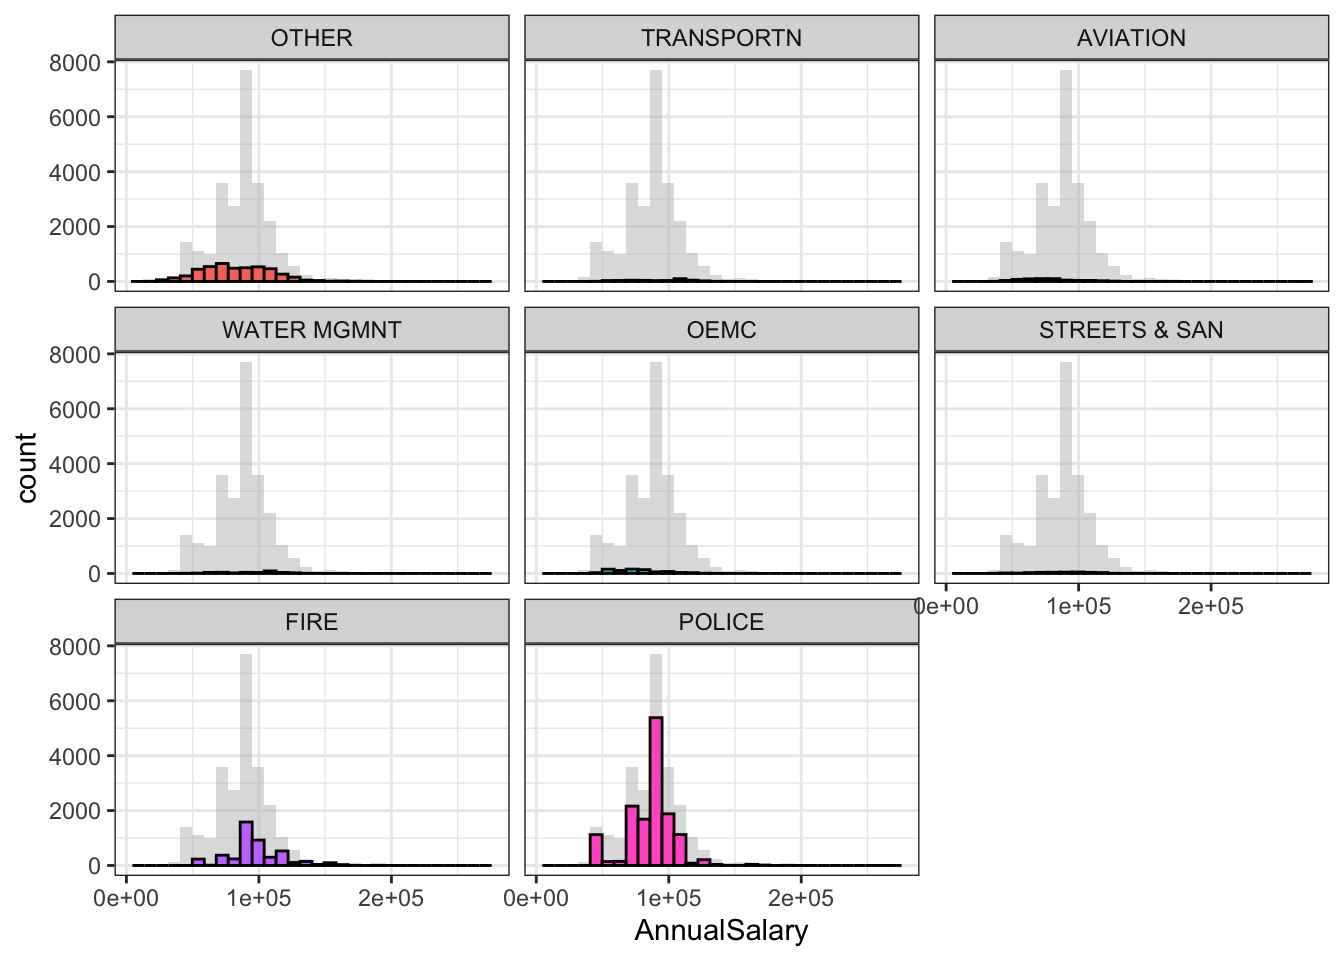
\includegraphics{gggallery_files/figure-latex/unnamed-chunk-82-1.pdf}
To add the text, \emph{annotate} can be used again. This time with the \emph{geom} argument set to ``text''.

\begin{Shaded}
\begin{Highlighting}[]
\NormalTok{sp_plt <-}\StringTok{ }\NormalTok{sp_plt }\OperatorTok{+}\StringTok{ }
\StringTok{  }\KeywordTok{annotate}\NormalTok{(}\StringTok{"text"}\NormalTok{, }\DataTypeTok{label =} \StringTok{"95th percentile"}\NormalTok{, }\DataTypeTok{y =}\NormalTok{ (pct95}\OperatorTok{+}\NormalTok{pct99)}\OperatorTok{/}\DecValTok{2}\NormalTok{, }\DataTypeTok{x =} \StringTok{"06-01"}\NormalTok{ ) }\OperatorTok{+}
\StringTok{  }\KeywordTok{annotate}\NormalTok{(}\StringTok{"text"}\NormalTok{, }\DataTypeTok{label =} \StringTok{"99th percentile"}\NormalTok{, }\DataTypeTok{y =}\NormalTok{ pct99 }\OperatorTok{+}\StringTok{ }\NormalTok{(pct99}\OperatorTok{-}\NormalTok{pct95)}\OperatorTok{/}\DecValTok{2}\NormalTok{, }\DataTypeTok{x =} \StringTok{"06-01"}\NormalTok{)}

\NormalTok{sp_plt}
\end{Highlighting}
\end{Shaded}

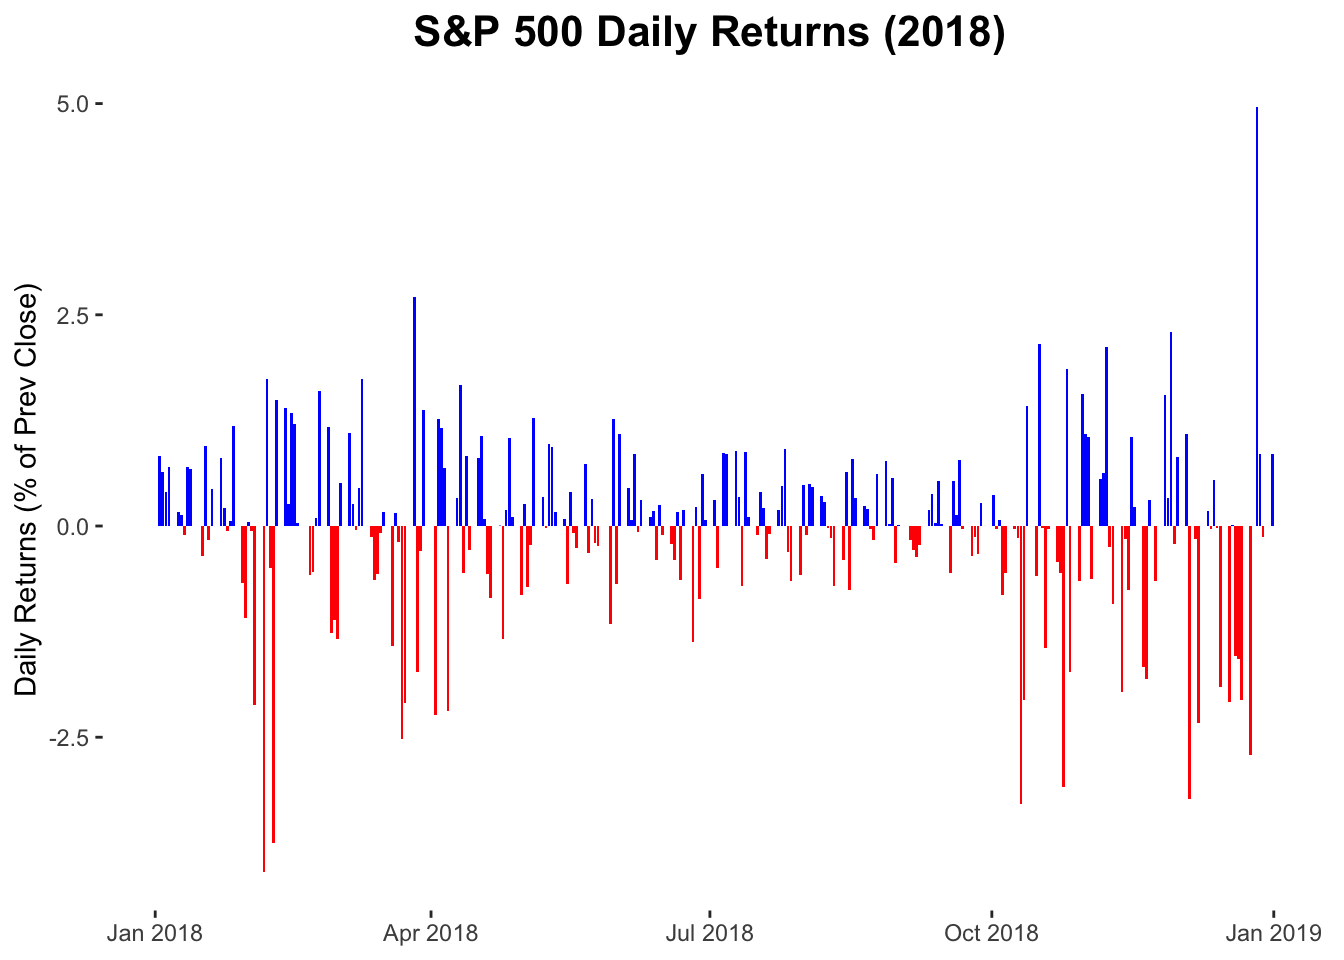
\includegraphics{gggallery_files/figure-latex/unnamed-chunk-83-1.pdf}

The complete code for the plot

\begin{Shaded}
\begin{Highlighting}[]
\NormalTok{sp_plt <-}\StringTok{ }\KeywordTok{ggplot}\NormalTok{(}\DataTypeTok{data =}\NormalTok{ df, }\KeywordTok{aes}\NormalTok{(}\DataTypeTok{x =}\NormalTok{ MonthDay, }\DataTypeTok{y =}\NormalTok{ daily_return)) }\OperatorTok{+}
\StringTok{  }\KeywordTok{geom_bar}\NormalTok{(}\DataTypeTok{stat =} \StringTok{"identity"}\NormalTok{) }\OperatorTok{+}
\StringTok{  }\KeywordTok{facet_wrap}\NormalTok{(}\OperatorTok{~}\NormalTok{Year) }\OperatorTok{+}\StringTok{ }
\StringTok{  }\KeywordTok{ylab}\NormalTok{(}\StringTok{"Daily Returns (% of Prev Close)"}\NormalTok{) }\OperatorTok{+}
\StringTok{  }\KeywordTok{ggtitle}\NormalTok{(}\StringTok{"S&P 500 Daily Returns (2015 - 2018)"}\NormalTok{) }\OperatorTok{+}\StringTok{ }
\StringTok{  }\KeywordTok{theme}\NormalTok{(}\DataTypeTok{plot.title =} \KeywordTok{element_text}\NormalTok{(}\DataTypeTok{size =} \DecValTok{16}\NormalTok{, }\DataTypeTok{face =} \StringTok{"bold"}\NormalTok{, }\DataTypeTok{hjust =} \FloatTok{0.5}\NormalTok{), }
        \DataTypeTok{panel.background =} \KeywordTok{element_blank}\NormalTok{(), }\DataTypeTok{axis.title.x=}\KeywordTok{element_blank}\NormalTok{(), }
        \DataTypeTok{axis.text.x =}  \KeywordTok{element_blank}\NormalTok{(), }\DataTypeTok{axis.ticks.x =} \KeywordTok{element_blank}\NormalTok{()) }\OperatorTok{+}\StringTok{ }
\StringTok{  }\KeywordTok{annotate}\NormalTok{(}\StringTok{"ribbon"}\NormalTok{, }\DataTypeTok{ymin =}\NormalTok{ pct95, }\DataTypeTok{ymax =}\NormalTok{ pct99, }\DataTypeTok{x =} \KeywordTok{c}\NormalTok{(}\OperatorTok{-}\OtherTok{Inf}\NormalTok{,}\OtherTok{Inf}\NormalTok{), }\DataTypeTok{alpha =} \FloatTok{0.3}\NormalTok{, }\DataTypeTok{fill =} \StringTok{"95"}\NormalTok{) }\OperatorTok{+}
\StringTok{  }\KeywordTok{annotate}\NormalTok{(}\StringTok{"ribbon"}\NormalTok{, }\DataTypeTok{ymin =}\NormalTok{ pct99, }\DataTypeTok{ymax =} \OtherTok{Inf}\NormalTok{, }\DataTypeTok{x =} \KeywordTok{c}\NormalTok{(}\OperatorTok{-}\OtherTok{Inf}\NormalTok{, }\OtherTok{Inf}\NormalTok{), }\DataTypeTok{alpha =} \FloatTok{0.3}\NormalTok{, }\DataTypeTok{fill =} \StringTok{"99"}\NormalTok{) }\OperatorTok{+}\StringTok{ }
\StringTok{  }\KeywordTok{annotate}\NormalTok{(}\StringTok{"ribbon"}\NormalTok{, }\DataTypeTok{ymax =} \OperatorTok{-}\NormalTok{pct95, }\DataTypeTok{ymin =} \OperatorTok{-}\NormalTok{pct99, }\DataTypeTok{x =} \KeywordTok{c}\NormalTok{(}\OperatorTok{-}\OtherTok{Inf}\NormalTok{,}\OtherTok{Inf}\NormalTok{), }\DataTypeTok{alpha =} \FloatTok{0.3}\NormalTok{, }\DataTypeTok{fill =} \StringTok{"95"}\NormalTok{) }\OperatorTok{+}\StringTok{ }
\StringTok{  }\KeywordTok{annotate}\NormalTok{(}\StringTok{"ribbon"}\NormalTok{, }\DataTypeTok{ymax =} \OperatorTok{-}\NormalTok{pct99, }\DataTypeTok{ymin =} \OperatorTok{-}\OtherTok{Inf}\NormalTok{, }\DataTypeTok{x =} \KeywordTok{c}\NormalTok{(}\OperatorTok{-}\OtherTok{Inf}\NormalTok{, }\OtherTok{Inf}\NormalTok{), }\DataTypeTok{alpha =} \FloatTok{0.3}\NormalTok{, }\DataTypeTok{fill =} \StringTok{"99"}\NormalTok{) }\OperatorTok{+}
\StringTok{  }\KeywordTok{annotate}\NormalTok{(}\StringTok{"text"}\NormalTok{, }\DataTypeTok{label =} \StringTok{"95th percentile"}\NormalTok{, }\DataTypeTok{y =}\NormalTok{ (pct95}\OperatorTok{+}\NormalTok{pct99)}\OperatorTok{/}\DecValTok{2}\NormalTok{, }\DataTypeTok{x =} \StringTok{"06-01"}\NormalTok{ ) }\OperatorTok{+}
\StringTok{  }\KeywordTok{annotate}\NormalTok{(}\StringTok{"text"}\NormalTok{, }\DataTypeTok{label =} \StringTok{"99th percentile"}\NormalTok{, }\DataTypeTok{y =}\NormalTok{ pct99 }\OperatorTok{+}\StringTok{ }\NormalTok{(pct99}\OperatorTok{-}\NormalTok{pct95)}\OperatorTok{/}\DecValTok{2}\NormalTok{, }\DataTypeTok{x =} \StringTok{"06-01"}\NormalTok{)}

\NormalTok{sp_plt}
\end{Highlighting}
\end{Shaded}

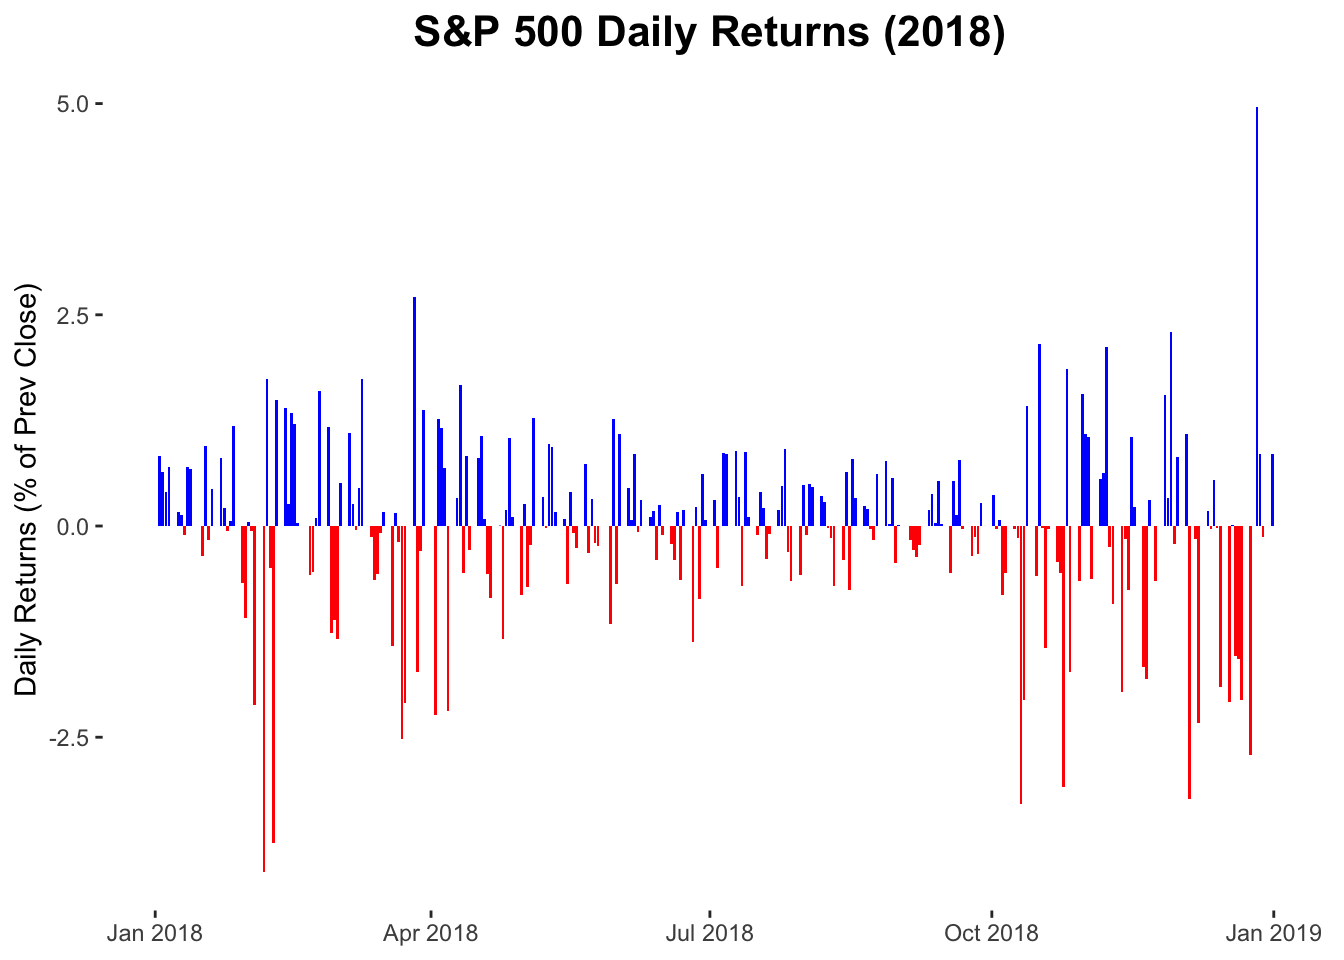
\includegraphics{gggallery_files/figure-latex/unnamed-chunk-84-1.pdf}

\hypertarget{tfwr}{%
\chapter*{World Record Progression}\label{tfwr}}
\addcontentsline{toc}{chapter}{World Record Progression}

\hypertarget{tfwrdata}{%
\subsubsection*{Data}\label{tfwrdata}}
\addcontentsline{toc}{subsubsection}{Data}

This plot uses the \emph{wr} data frame of the \emph{gcubed} package.

\begin{Shaded}
\begin{Highlighting}[]
\KeywordTok{head}\NormalTok{(wr)}
\end{Highlighting}
\end{Shaded}

\begin{verbatim}
## # A tibble: 6 x 6
##   Event    WR      Athlete                Location         Date       MF   
##   <chr>    <chr>   <chr>                  <chr>            <date>     <chr>
## 1 100 M    9.58    Usain Bolt (Jamaica)   Berlin, Germany  2009-08-16 M    
## 2 200 M    19.19   Usain Bolt (Jamaica)   Berlin, Germany  2009-08-20 M    
## 3 400 M    43.03   Wayde van Niekerk (So~ Rio de Janeiro,~ 2016-08-14 M    
## 4 800 M    01:40.9 David Rudisha (Kenya)  London, England  2012-08-09 M    
## 5 1500 M   03:26.0 Hicham El Guerrouj (M~ Rome, Italy      1998-07-14 M    
## 6 Steeple~ 07:53.6 Saïf Shaheen (Qatar)   Brussels, Belgi~ 2004-09-03 M
\end{verbatim}

\hypertarget{tfwrcode}{%
\subsubsection*{Code for plot}\label{tfwrcode}}
\addcontentsline{toc}{subsubsection}{Code for plot}

This plot uses \emph{geom\_segment} geometry.

\begin{Shaded}
\begin{Highlighting}[]
\KeywordTok{library}\NormalTok{(ggplot2)}
\KeywordTok{library}\NormalTok{(dplyr) }\CommentTok{# used for arrange which sorts data by date}

\NormalTok{today <-}\StringTok{ }\KeywordTok{as.Date}\NormalTok{(}\StringTok{"2019-08-08"}\NormalTok{)}
\NormalTok{wr <-}\StringTok{ }\KeywordTok{arrange}\NormalTok{(wr, }\KeywordTok{desc}\NormalTok{(Date)) }
\NormalTok{wr}\OperatorTok{$}\NormalTok{Event <-}\StringTok{ }\KeywordTok{factor}\NormalTok{(wr}\OperatorTok{$}\NormalTok{Event, }\DataTypeTok{levels =}\NormalTok{ wr}\OperatorTok{$}\NormalTok{Event)}
\NormalTok{wr}\OperatorTok{$}\NormalTok{MF2 <-}\StringTok{ }\KeywordTok{ifelse}\NormalTok{(wr}\OperatorTok{$}\NormalTok{MF }\OperatorTok{==}\StringTok{ "M"}\NormalTok{, }\StringTok{"Men"}\NormalTok{, }\StringTok{"Women"}\NormalTok{)}

\NormalTok{wr_plt <-}\StringTok{ }\KeywordTok{ggplot}\NormalTok{(wr, }\KeywordTok{aes}\NormalTok{(}\DataTypeTok{x =}\NormalTok{ Date, }\DataTypeTok{y =}\NormalTok{ Event)) }\OperatorTok{+}\StringTok{ }
\StringTok{  }\KeywordTok{geom_segment}\NormalTok{(}\KeywordTok{aes}\NormalTok{(}\DataTypeTok{x =}\NormalTok{ Date, }\DataTypeTok{xend =}\NormalTok{ today, }\DataTypeTok{y =}\NormalTok{ Event, }\DataTypeTok{yend =}\NormalTok{ Event, }\DataTypeTok{colour =}\NormalTok{ MF2), }\DataTypeTok{size =} \DecValTok{2}\NormalTok{) }\OperatorTok{+}
\StringTok{  }\KeywordTok{ggtitle}\NormalTok{(}\StringTok{"Longevity of Current Track & Field World Records"}\NormalTok{) }\OperatorTok{+}\StringTok{ }
\StringTok{  }\KeywordTok{theme_bw}\NormalTok{() }\OperatorTok{+}\StringTok{ }
\StringTok{  }\KeywordTok{theme}\NormalTok{(}\DataTypeTok{legend.title =} \KeywordTok{element_blank}\NormalTok{(),}
        \DataTypeTok{axis.title.y =} \KeywordTok{element_blank}\NormalTok{(),}
        \DataTypeTok{plot.title =} \KeywordTok{element_text}\NormalTok{(}\DataTypeTok{size =} \DecValTok{16}\NormalTok{, }\DataTypeTok{face =} \StringTok{"bold"}\NormalTok{, }\DataTypeTok{hjust =} \FloatTok{0.5}\NormalTok{)) }\OperatorTok{+}\StringTok{ }
\StringTok{  }\KeywordTok{xlab}\NormalTok{(}\StringTok{"Date Record Set"}\NormalTok{)}

\NormalTok{wr_plt }
\end{Highlighting}
\end{Shaded}

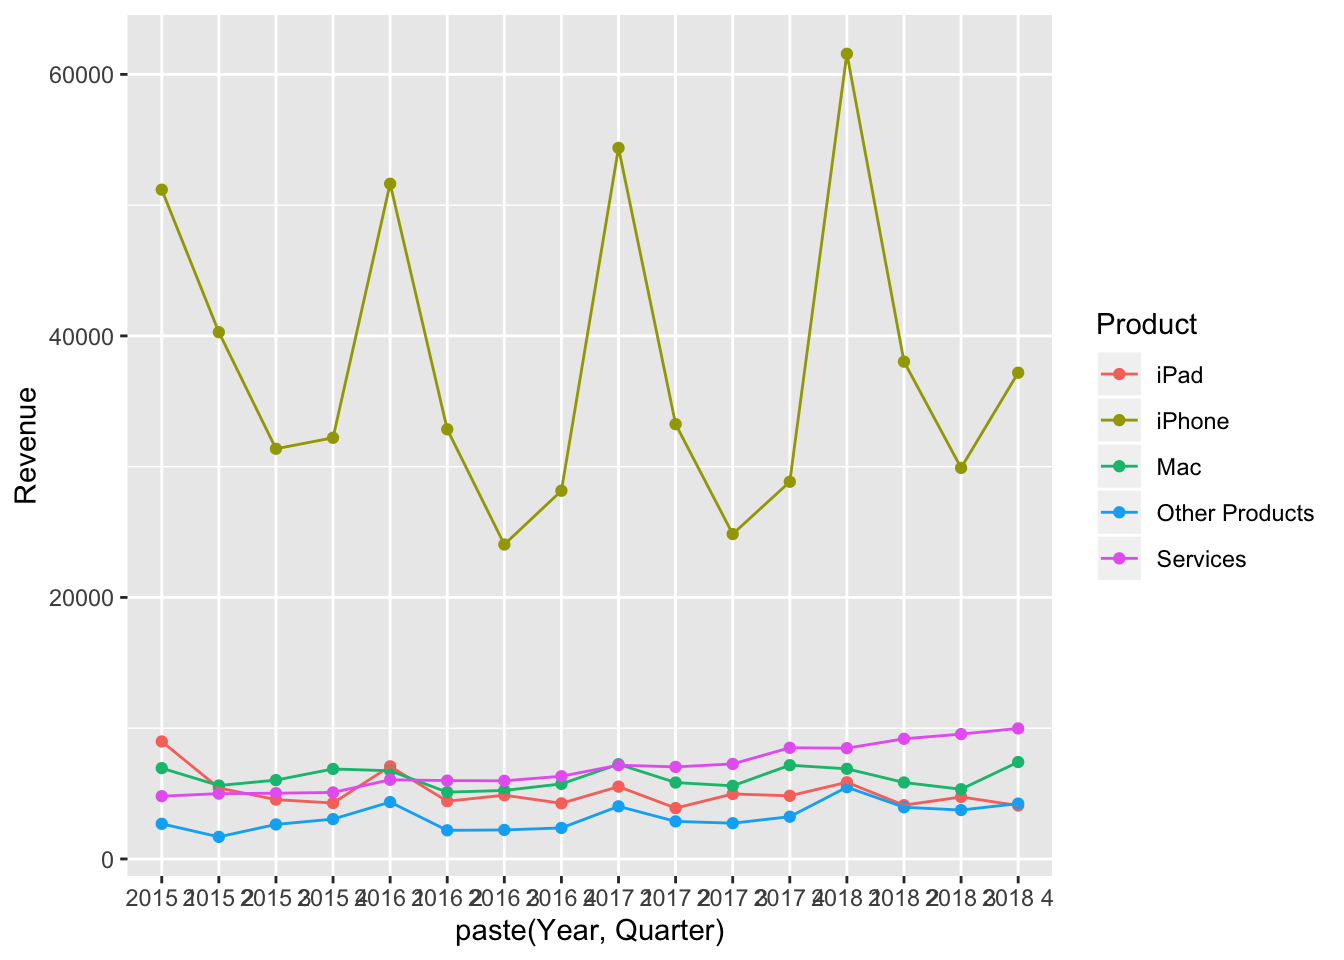
\includegraphics{gggallery_files/figure-latex/unnamed-chunk-88-1.pdf}

\hypertarget{lifeexcountries}{%
\chapter*{Life Expectancy for Selected Countries}\label{lifeexcountries}}
\addcontentsline{toc}{chapter}{Life Expectancy for Selected Countries}

\hypertarget{lifeexcountriesdata}{%
\subsubsection*{Data}\label{lifeexcountriesdata}}
\addcontentsline{toc}{subsubsection}{Data}

This plot uses the \emph{life\_ex} and \emph{regions} data frames of the \emph{gcubed} package.

\begin{Shaded}
\begin{Highlighting}[]
\NormalTok{le <-}\StringTok{ }\KeywordTok{inner_join}\NormalTok{(life_ex, regions, }\DataTypeTok{by =} \KeywordTok{c}\NormalTok{(}\StringTok{"Entity"}\NormalTok{ =}\StringTok{ "country"}\NormalTok{)) }\OperatorTok
\StringTok{  }\KeywordTok{filter}\NormalTok{(Year }\OperatorTok{==}\StringTok{ }\DecValTok{1950} \OperatorTok{|}\StringTok{ }\NormalTok{Year }\OperatorTok{==}\StringTok{ }\DecValTok{2015}\NormalTok{) }
\end{Highlighting}
\end{Shaded}

\begin{Shaded}
\begin{Highlighting}[]
\KeywordTok{library}\NormalTok{(dplyr)}
\NormalTok{income_levels <-}\StringTok{ }\KeywordTok{c}\NormalTok{(}\StringTok{"Low income"}\NormalTok{, }\StringTok{"Lower middle income"}\NormalTok{,}
                            \StringTok{"Upper middle income"}\NormalTok{, }\StringTok{"High income"}\NormalTok{)}
\NormalTok{le}\OperatorTok{$}\NormalTok{incomegroup <-}\StringTok{ }\KeywordTok{factor}\NormalTok{(le}\OperatorTok{$}\NormalTok{incomegroup, }\DataTypeTok{levels =}\NormalTok{ income_levels)}


\NormalTok{le <-}\StringTok{ }\NormalTok{le }\OperatorTok\StringTok{  }\KeywordTok{spread}\NormalTok{(}\DataTypeTok{key =}\NormalTok{ Year, }\DataTypeTok{value =}\NormalTok{ LE) }\OperatorTok
\StringTok{  }\KeywordTok{arrange}\NormalTok{(incomegroup, Entity) }

\NormalTok{country_levels <-}\StringTok{ }\NormalTok{le}\OperatorTok{$}\NormalTok{Entity}
\NormalTok{le}\OperatorTok{$}\NormalTok{country <-}\StringTok{ }\KeywordTok{factor}\NormalTok{(le}\OperatorTok{$}\NormalTok{Entity, }\DataTypeTok{levels =}\NormalTok{ country_levels)}
\end{Highlighting}
\end{Shaded}

\begin{Shaded}
\begin{Highlighting}[]
\NormalTok{le_plt <-}\StringTok{ }\KeywordTok{ggplot}\NormalTok{() }\OperatorTok{+}
\StringTok{  }\KeywordTok{geom_segment}\NormalTok{(}\DataTypeTok{data=}\NormalTok{le, }\DataTypeTok{mapping=}\KeywordTok{aes}\NormalTok{(}\DataTypeTok{x=}\NormalTok{country, }\DataTypeTok{xend=}\NormalTok{country,}
                                    \DataTypeTok{y =} \StringTok{`}\DataTypeTok{1950}\StringTok{`}\NormalTok{, }\DataTypeTok{yend=}\StringTok{`}\DataTypeTok{2015}\StringTok{`}\NormalTok{) ) }\OperatorTok{+}
\StringTok{  }\KeywordTok{geom_point}\NormalTok{(}\DataTypeTok{data =}\NormalTok{ le, }\KeywordTok{aes}\NormalTok{(}\DataTypeTok{x =}\NormalTok{ country, }\DataTypeTok{y =} \StringTok{`}\DataTypeTok{1950}\StringTok{`}\NormalTok{, }\DataTypeTok{colour =} \StringTok{"1950"}\NormalTok{)) }\OperatorTok{+}
\StringTok{  }\KeywordTok{geom_point}\NormalTok{(}\DataTypeTok{data =}\NormalTok{ le, }\KeywordTok{aes}\NormalTok{(}\DataTypeTok{x =}\NormalTok{ country, }\DataTypeTok{y =} \StringTok{`}\DataTypeTok{2015}\StringTok{`}\NormalTok{, }\DataTypeTok{colour =} \StringTok{"2015"}\NormalTok{)) }\OperatorTok{+}
\StringTok{  }\KeywordTok{theme_bw}\NormalTok{() }\OperatorTok{+}
\StringTok{  }\KeywordTok{scale_x_discrete}\NormalTok{(}\DataTypeTok{labels=}\NormalTok{country_levels)}\OperatorTok{+}
\StringTok{  }\KeywordTok{ylab}\NormalTok{(}\StringTok{"Life Expectancy (years)"}\NormalTok{) }\OperatorTok{+}
\StringTok{  }\KeywordTok{ggtitle}\NormalTok{(}\StringTok{"Global Life Expectancy (1950 - 2015)"}\NormalTok{) }\OperatorTok{+}
\StringTok{  }\KeywordTok{scale_colour_manual}\NormalTok{(}\DataTypeTok{values =} \KeywordTok{c}\NormalTok{(}\StringTok{"grey"}\NormalTok{, }\StringTok{"royalblue"}\NormalTok{), }\DataTypeTok{name =} \StringTok{""}\NormalTok{) }
  
\NormalTok{le_plt}
\end{Highlighting}
\end{Shaded}

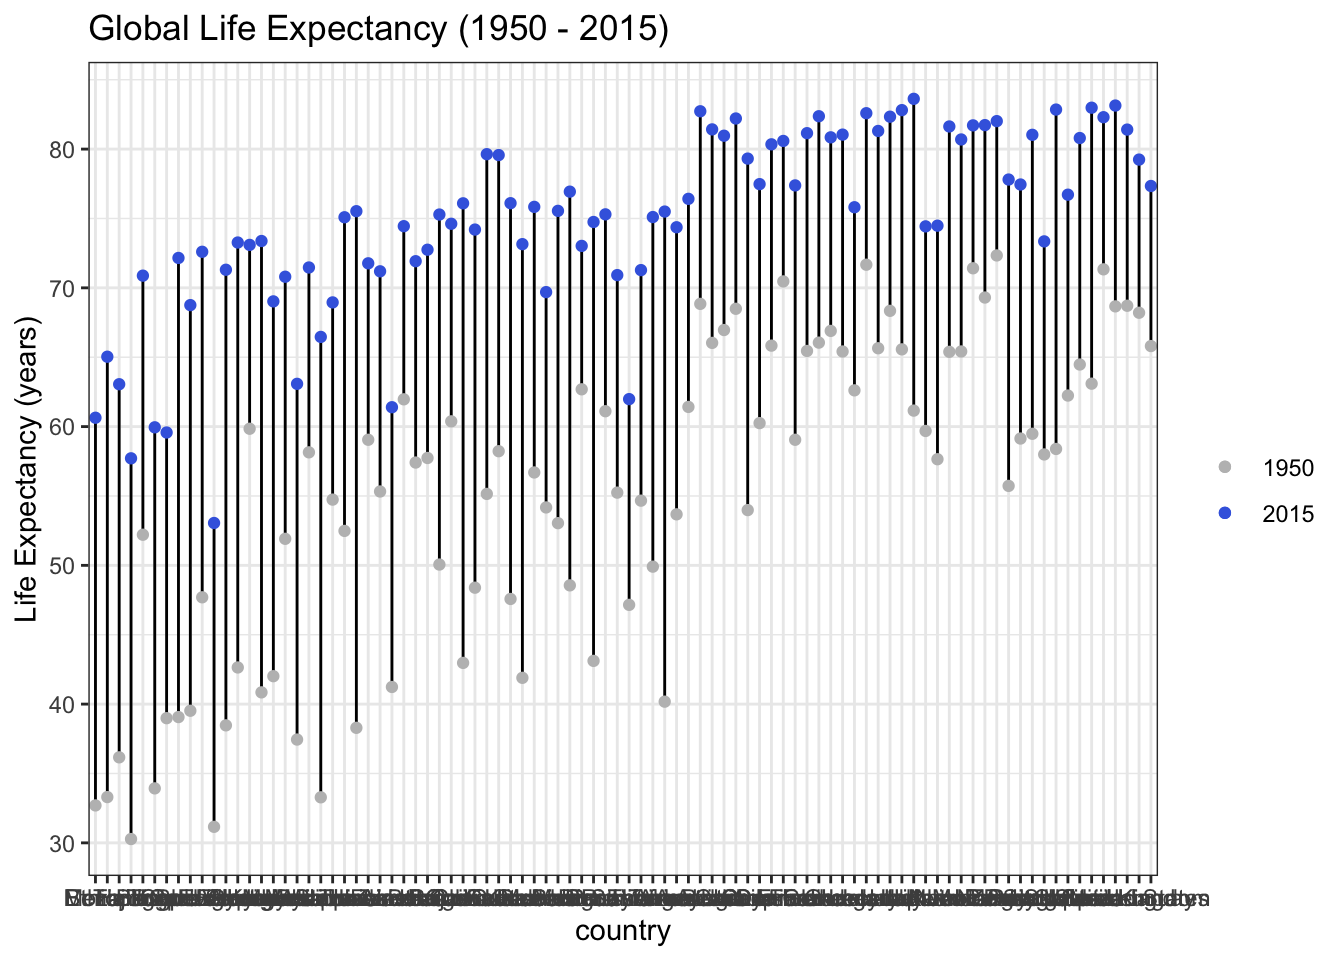
\includegraphics{gggallery_files/figure-latex/unnamed-chunk-93-1.pdf}

\begin{Shaded}
\begin{Highlighting}[]
\NormalTok{le_plt <-}\StringTok{ }\NormalTok{le_plt }\OperatorTok{+}\StringTok{ }
\StringTok{    }\KeywordTok{theme}\NormalTok{(}\DataTypeTok{axis.title.x=}\KeywordTok{element_blank}\NormalTok{(),}
        \DataTypeTok{axis.text.x =} \KeywordTok{element_text}\NormalTok{(}\DataTypeTok{hjust =} \DecValTok{1}\NormalTok{, }\DataTypeTok{angle =} \DecValTok{90}\NormalTok{, }\DataTypeTok{vjust=}\FloatTok{0.1}\NormalTok{),}
        \DataTypeTok{axis.ticks.y =} \KeywordTok{element_blank}\NormalTok{(),}
        \DataTypeTok{panel.grid.minor.y =} \KeywordTok{element_blank}\NormalTok{(),}
        \DataTypeTok{legend.title =} \KeywordTok{element_blank}\NormalTok{(),}
        \DataTypeTok{plot.title =} \KeywordTok{element_text}\NormalTok{(}\DataTypeTok{size =} \DecValTok{16}\NormalTok{, }\DataTypeTok{face =} \StringTok{"bold"}\NormalTok{, }\DataTypeTok{hjust =} \FloatTok{0.5}\NormalTok{))}

\NormalTok{le_plt}
\end{Highlighting}
\end{Shaded}

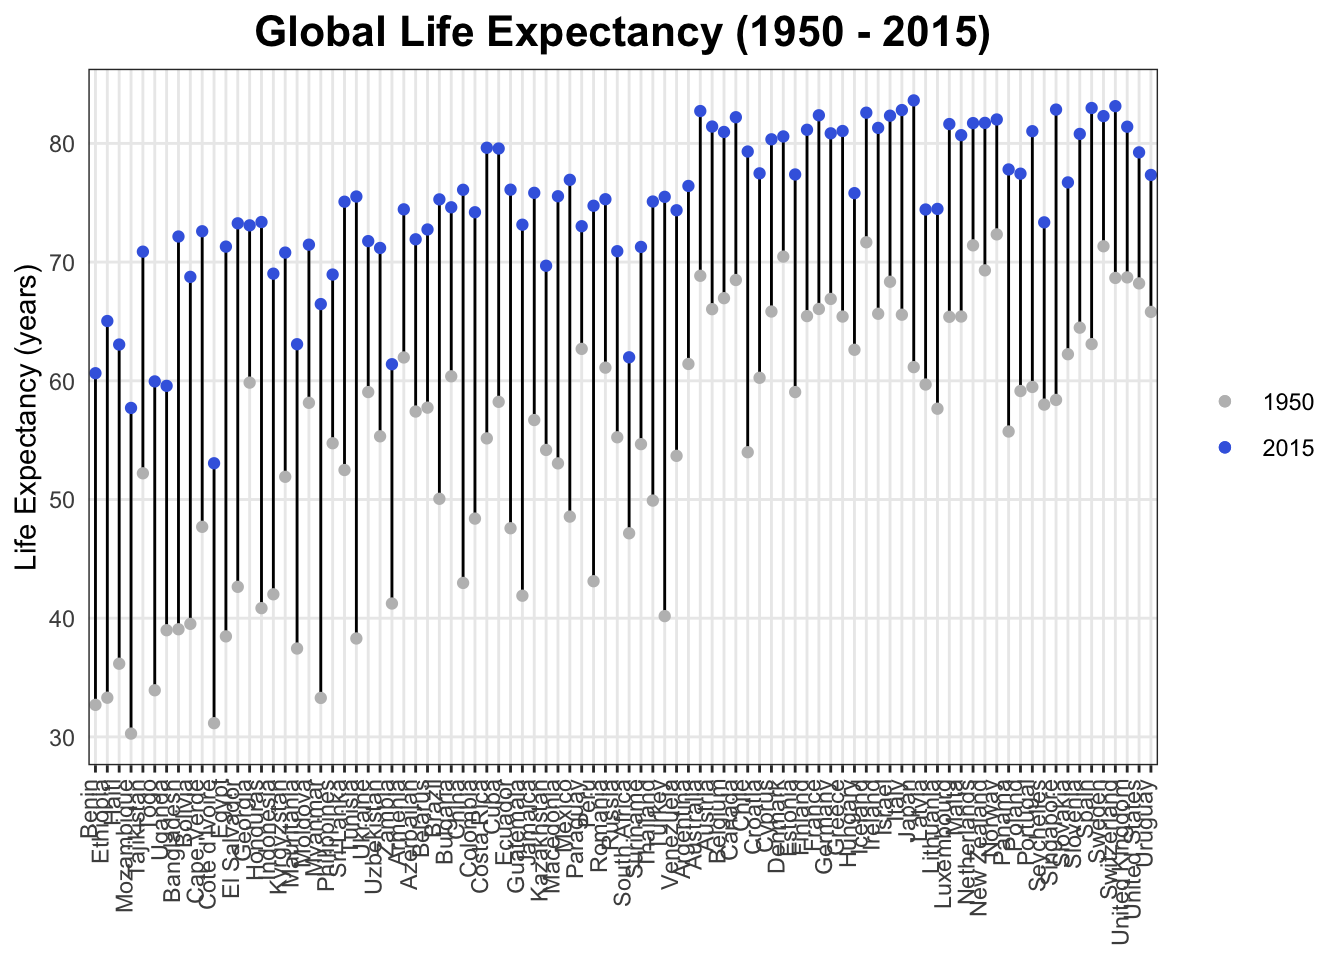
\includegraphics{gggallery_files/figure-latex/unnamed-chunk-94-1.pdf}

\begin{Shaded}
\begin{Highlighting}[]
\KeywordTok{cumsum}\NormalTok{(}\KeywordTok{table}\NormalTok{(le}\OperatorTok{$}\NormalTok{incomegroup))}
\end{Highlighting}
\end{Shaded}

\begin{verbatim}
##          Low income Lower middle income Upper middle income 
##                   7                  26                  50 
##         High income 
##                  90
\end{verbatim}

Adding dividing lines between the income groups using \emph{geom\_vline}:

\begin{Shaded}
\begin{Highlighting}[]
\NormalTok{le_plt <-}\StringTok{ }\NormalTok{le_plt }\OperatorTok{+}
\StringTok{  }\KeywordTok{geom_vline}\NormalTok{(}\DataTypeTok{xintercept =} \FloatTok{7.5}\NormalTok{, }\DataTypeTok{linetype =} \StringTok{"dashed"}\NormalTok{, }\DataTypeTok{colour =} \StringTok{"grey"}\NormalTok{) }\OperatorTok{+}
\StringTok{  }\KeywordTok{geom_vline}\NormalTok{(}\DataTypeTok{xintercept =} \FloatTok{26.5}\NormalTok{, }\DataTypeTok{linetype =} \StringTok{"dashed"}\NormalTok{, }\DataTypeTok{colour =} \StringTok{"grey"}\NormalTok{) }\OperatorTok{+}
\StringTok{  }\KeywordTok{geom_vline}\NormalTok{(}\DataTypeTok{xintercept =} \FloatTok{50.5}\NormalTok{, }\DataTypeTok{linetype =} \StringTok{"dashed"}\NormalTok{, }\DataTypeTok{colour =} \StringTok{"grey"}\NormalTok{)}

\NormalTok{le_plt }
\end{Highlighting}
\end{Shaded}

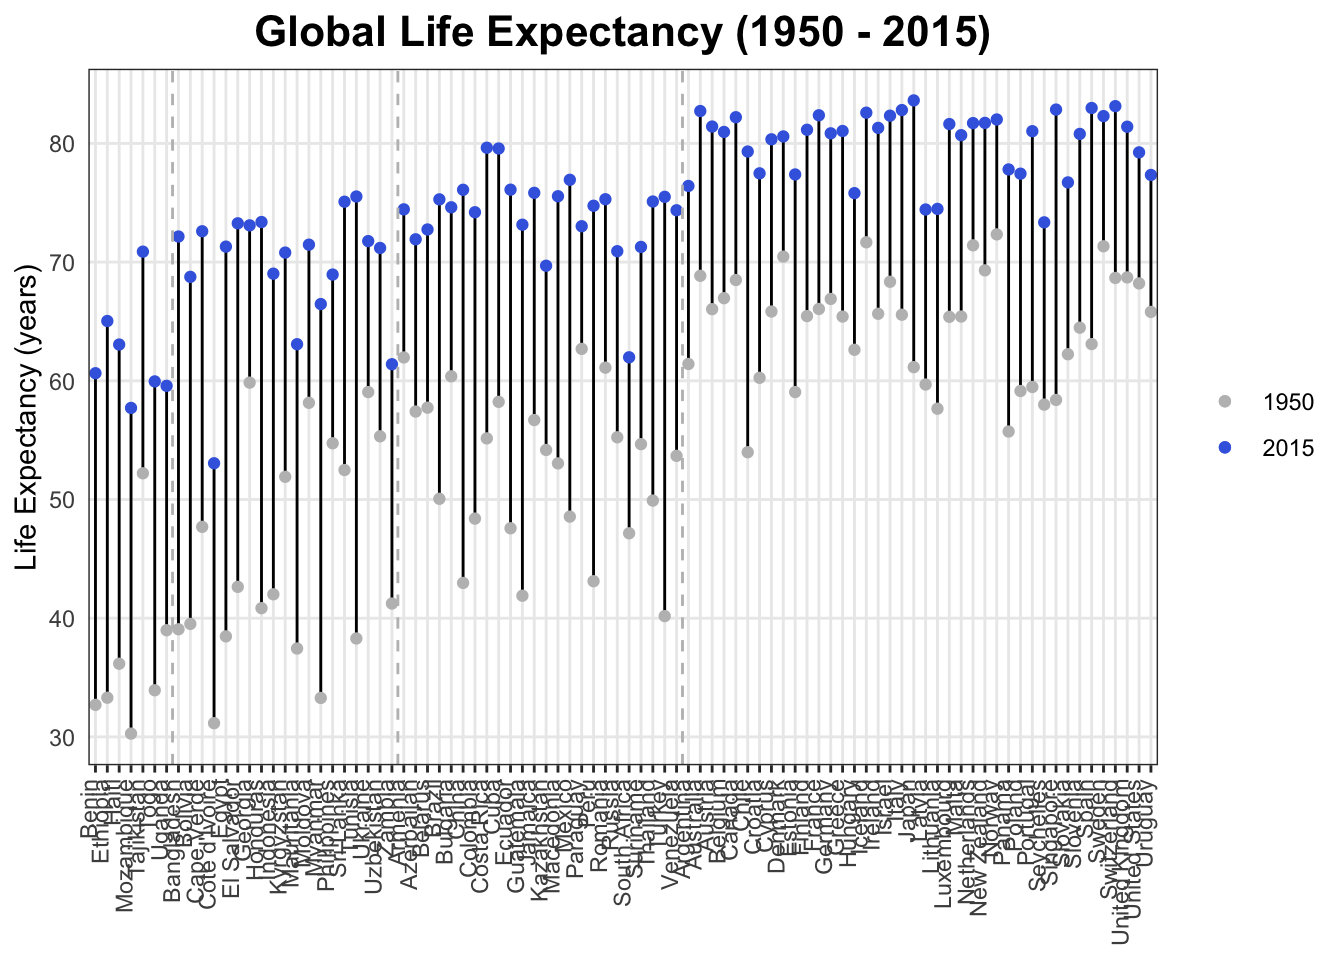
\includegraphics{gggallery_files/figure-latex/unnamed-chunk-96-1.pdf}

Adding the text for the income groups using \emph{geom\_text}:

\begin{Shaded}
\begin{Highlighting}[]
\NormalTok{le_plt <-}\StringTok{ }\NormalTok{le_plt }\OperatorTok{+}\StringTok{ }
\StringTok{  }\KeywordTok{geom_text}\NormalTok{(}\KeywordTok{aes}\NormalTok{(}\DecValTok{4}\NormalTok{,}\DecValTok{87}\NormalTok{,}\DataTypeTok{label =} \StringTok{"Low Income"}\NormalTok{), }\DataTypeTok{colour =} \StringTok{"red"}\NormalTok{) }\OperatorTok{+}
\StringTok{  }\KeywordTok{geom_text}\NormalTok{(}\KeywordTok{aes}\NormalTok{(}\DecValTok{15}\NormalTok{,}\DecValTok{87}\NormalTok{,}\DataTypeTok{label =} \StringTok{"Lower middle income"}\NormalTok{), }\DataTypeTok{colour =} \StringTok{"red"}\NormalTok{) }\OperatorTok{+}
\StringTok{  }\KeywordTok{geom_text}\NormalTok{(}\KeywordTok{aes}\NormalTok{(}\DecValTok{35}\NormalTok{,}\DecValTok{87}\NormalTok{,}\DataTypeTok{label =} \StringTok{"Upper middle income"}\NormalTok{), }\DataTypeTok{colour =} \StringTok{"red"}\NormalTok{) }\OperatorTok{+}
\StringTok{  }\KeywordTok{geom_text}\NormalTok{(}\KeywordTok{aes}\NormalTok{(}\DecValTok{60}\NormalTok{,}\DecValTok{87}\NormalTok{,}\DataTypeTok{label =} \StringTok{"High income"}\NormalTok{), }\DataTypeTok{colour =} \StringTok{"red"}\NormalTok{)}

\NormalTok{le_plt }
\end{Highlighting}
\end{Shaded}

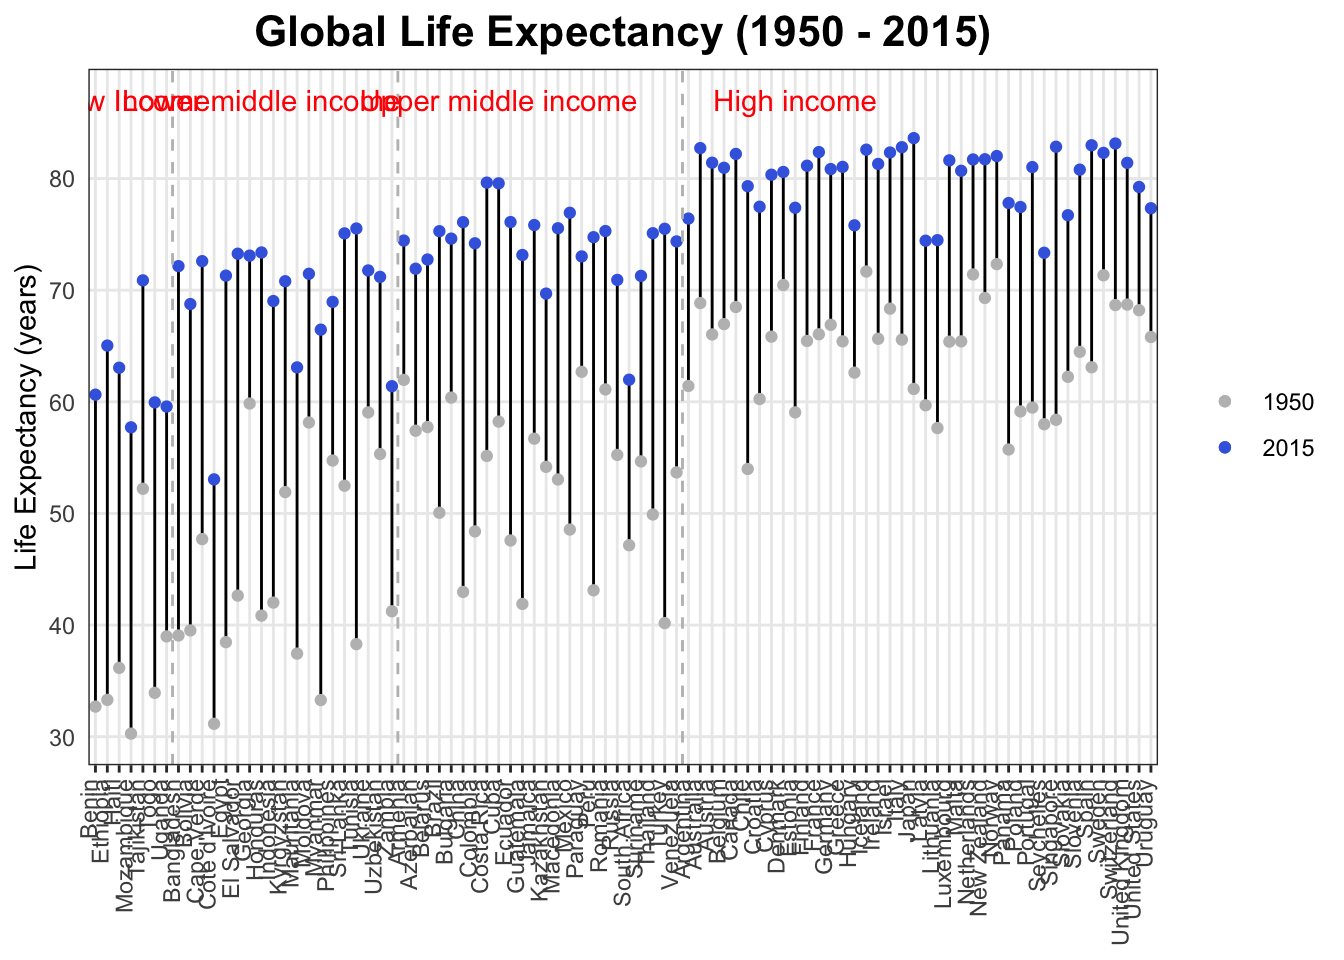
\includegraphics{gggallery_files/figure-latex/unnamed-chunk-97-1.pdf}

\hypertarget{metsbar}{%
\chapter*{NY Mets 2019 Season}\label{metsbar}}
\addcontentsline{toc}{chapter}{NY Mets 2019 Season}

\hypertarget{metsbardata}{%
\subsubsection*{Data}\label{metsbardata}}
\addcontentsline{toc}{subsubsection}{Data}

This plot uses the \emph{nym} data frame of the \emph{gcubed} package.

\begin{Shaded}
\begin{Highlighting}[]
\KeywordTok{head}\NormalTok{(nym)}
\end{Highlighting}
\end{Shaded}

\begin{verbatim}
## # A tibble: 6 x 24
##   `Gm#` Weekday Month Day   Tm    X5    Opp   WL    wo        R    RA   Inn
##   <dbl> <chr>   <chr> <chr> <chr> <chr> <chr> <chr> <chr> <dbl> <dbl> <dbl>
## 1     1 Thursd~ Mar   28    NYM   @     WSN   W     <NA>      2     0    NA
## 2     2 Saturd~ Mar   30    NYM   @     WSN   W     <NA>     11     8    NA
## 3     3 Sunday  Mar   31    NYM   @     WSN   L     wo        5     6    NA
## 4     4 Monday  Apr   1     NYM   @     MIA   W     <NA>      7     3    NA
## 5     5 Tuesday Apr   2     NYM   @     MIA   W     <NA>      6     5    NA
## 6     6 Wednes~ Apr   3     NYM   @     MIA   W     <NA>      6     4    NA
## # ... with 12 more variables: `W-L` <chr>, Rank <dbl>, GB <chr>,
## #   Win <chr>, Loss <chr>, Save <chr>, Time <drtn>, `D/N` <chr>,
## #   Attendance <dbl>, Streak <chr>, `Orig. Scheduled` <lgl>,
## #   HomeAway <chr>
\end{verbatim}

\hypertarget{metsbarcode}{%
\subsubsection*{Code for plot}\label{metsbarcode}}
\addcontentsline{toc}{subsubsection}{Code for plot}

\begin{Shaded}
\begin{Highlighting}[]
\NormalTok{mets_plt <-}\StringTok{ }\KeywordTok{ggplot}\NormalTok{(nym, }\KeywordTok{aes}\NormalTok{(}\DataTypeTok{x =} \StringTok{`}\DataTypeTok{Gm#}\StringTok{`}\NormalTok{, }\DataTypeTok{y =} \KeywordTok{ifelse}\NormalTok{(WL }\OperatorTok{==}\StringTok{ "W"}\NormalTok{, }\DecValTok{1}\NormalTok{,}\OperatorTok{-}\DecValTok{1}\NormalTok{), }\DataTypeTok{fill =}\NormalTok{ WL) ) }\OperatorTok{+}\StringTok{ }
\StringTok{  }\KeywordTok{geom_bar}\NormalTok{(}\DataTypeTok{stat =} \StringTok{"identity"}\NormalTok{) }\OperatorTok{+}\StringTok{ }
\StringTok{  }\KeywordTok{scale_fill_manual}\NormalTok{(}\DataTypeTok{values =} \KeywordTok{c}\NormalTok{(}\StringTok{"#FF5910"}\NormalTok{, }\StringTok{"#002D72"}\NormalTok{)) }\OperatorTok{+}\StringTok{ }
\StringTok{  }\KeywordTok{xlab}\NormalTok{(}\StringTok{"Game #"}\NormalTok{) }\OperatorTok{+}
\StringTok{  }\KeywordTok{ggtitle}\NormalTok{(}\StringTok{"NY Mets Season Results (2019"}\NormalTok{) }\OperatorTok{+}\StringTok{ }
\StringTok{  }\KeywordTok{theme}\NormalTok{(}\DataTypeTok{panel.background =} \KeywordTok{element_blank}\NormalTok{(),}
        \DataTypeTok{axis.title.y =} \KeywordTok{element_blank}\NormalTok{(),}
        \DataTypeTok{legend.title =} \KeywordTok{element_blank}\NormalTok{(),}
        \DataTypeTok{axis.text.y =} \KeywordTok{element_blank}\NormalTok{(),}
        \DataTypeTok{axis.ticks.y =} \KeywordTok{element_blank}\NormalTok{(), }
        \DataTypeTok{plot.title =} \KeywordTok{element_text}\NormalTok{(}\DataTypeTok{size =} \DecValTok{16}\NormalTok{, }\DataTypeTok{face =} \StringTok{"bold"}\NormalTok{, }\DataTypeTok{hjust =} \FloatTok{0.5}\NormalTok{)) }\OperatorTok{+}\StringTok{ }
\StringTok{  }\KeywordTok{guides}\NormalTok{(}\DataTypeTok{fill =} \KeywordTok{guide_legend}\NormalTok{(}\DataTypeTok{reverse=}\OtherTok{TRUE}\NormalTok{))}

\NormalTok{mets_plt}
\end{Highlighting}
\end{Shaded}

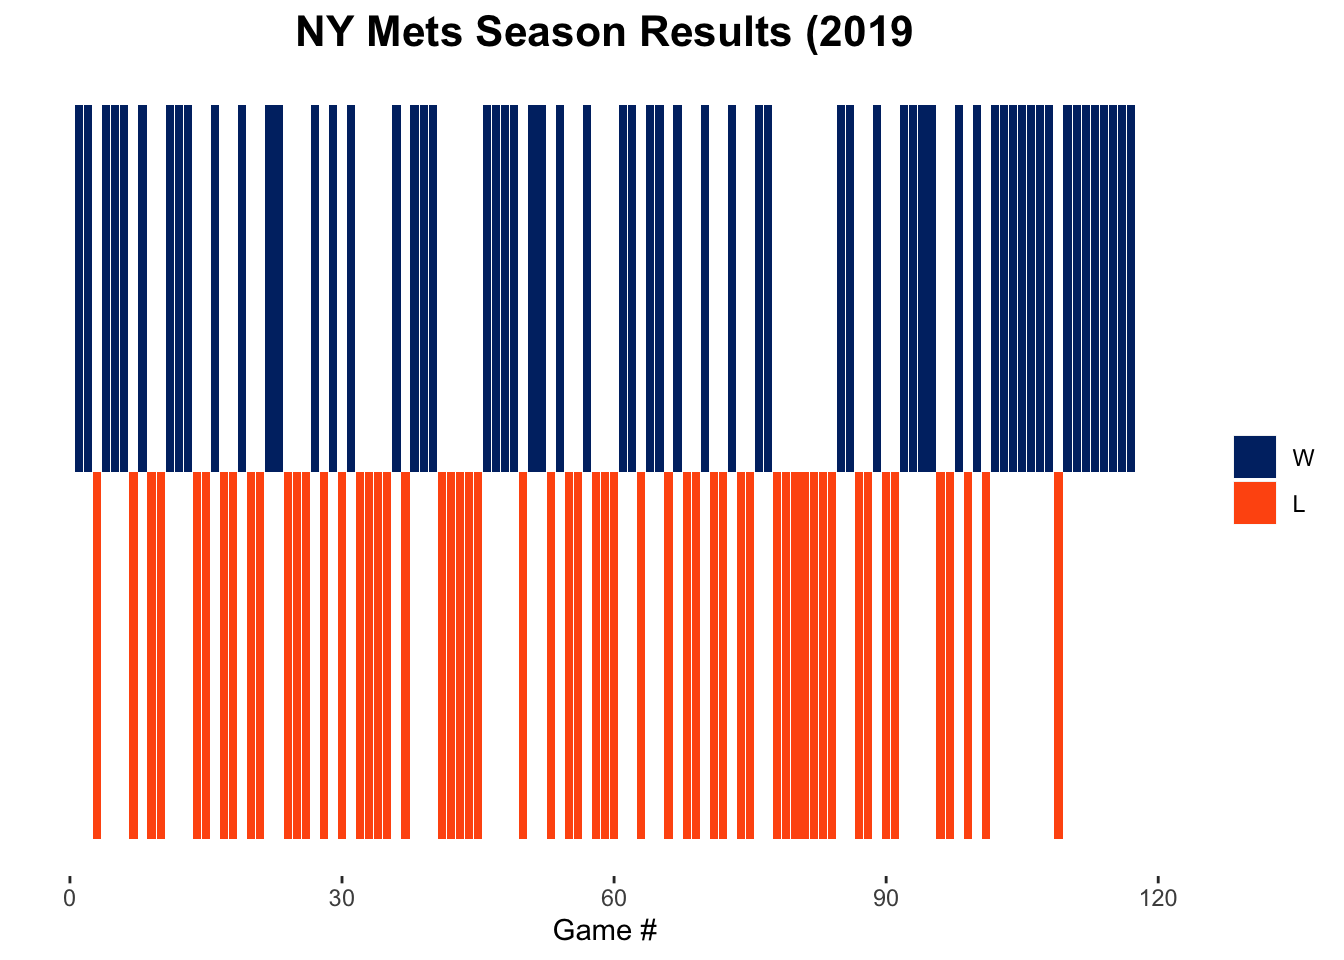
\includegraphics{gggallery_files/figure-latex/unnamed-chunk-102-1.pdf}

\hypertarget{nleastbars}{%
\chapter*{NL East 2019 Season Records}\label{nleastbars}}
\addcontentsline{toc}{chapter}{NL East 2019 Season Records}

\hypertarget{nleastbarsdata}{%
\subsubsection*{Data}\label{nleastbarsdata}}
\addcontentsline{toc}{subsubsection}{Data}

This plot uses the \emph{atl}, \emph{phi}, \emph{was}, \emph{nym} and \emph{mia} data frames of the \emph{gcubed} package.

\begin{Shaded}
\begin{Highlighting}[]
\NormalTok{nleast <-}\StringTok{ }\KeywordTok{bind_rows}\NormalTok{(atl, phi, was, nym, mia)}
\end{Highlighting}
\end{Shaded}

\hypertarget{nleastbarscode}{%
\subsubsection*{Code}\label{nleastbarscode}}
\addcontentsline{toc}{subsubsection}{Code}

\begin{Shaded}
\begin{Highlighting}[]
\NormalTok{nleast}\OperatorTok{$}\NormalTok{Tm <-}\StringTok{ }\KeywordTok{factor}\NormalTok{(nleast}\OperatorTok{$}\NormalTok{Tm, }\DataTypeTok{levels =} \KeywordTok{c}\NormalTok{(}\StringTok{"ATL"}\NormalTok{, }\StringTok{"WSN"}\NormalTok{, }\StringTok{"PHI"}\NormalTok{, }\StringTok{"NYM"}\NormalTok{, }\StringTok{"MIA"}\NormalTok{))}
\NormalTok{nlplot <-}\StringTok{ }\KeywordTok{ggplot}\NormalTok{(}\DataTypeTok{data =}\NormalTok{ nleast, }\KeywordTok{aes}\NormalTok{(}\DataTypeTok{x =} \StringTok{`}\DataTypeTok{Gm#}\StringTok{`}\NormalTok{, }\DataTypeTok{y =}\NormalTok{ win_updown,}
                          \DataTypeTok{fill =} \KeywordTok{factor}\NormalTok{(WL, }\DataTypeTok{levels =} \KeywordTok{c}\NormalTok{(}\StringTok{"W"}\NormalTok{, }\StringTok{"L"}\NormalTok{)))) }\OperatorTok{+}
\StringTok{  }\KeywordTok{geom_bar}\NormalTok{(}\DataTypeTok{stat =} \StringTok{"identity"}\NormalTok{) }\OperatorTok{+}
\StringTok{  }\KeywordTok{facet_wrap}\NormalTok{(}\OperatorTok{~}\NormalTok{Tm, }\DataTypeTok{ncol =} \DecValTok{1}\NormalTok{) }\OperatorTok{+}
\StringTok{  }\KeywordTok{scale_fill_manual}\NormalTok{(}\DataTypeTok{values =} \KeywordTok{c}\NormalTok{(}\StringTok{"royalblue"}\NormalTok{, }\StringTok{"peachpuff"}\NormalTok{), }\DataTypeTok{name =} \StringTok{""}\NormalTok{) }\OperatorTok{+}
\StringTok{  }\KeywordTok{theme_bw}\NormalTok{() }\OperatorTok{+}
\StringTok{  }\KeywordTok{ggtitle}\NormalTok{(}\StringTok{"NL East 2019"}\NormalTok{) }\OperatorTok{+}
\StringTok{  }\KeywordTok{xlab}\NormalTok{(}\StringTok{"Game #"}\NormalTok{) }\OperatorTok{+}
\StringTok{  }\KeywordTok{theme}\NormalTok{(}\DataTypeTok{axis.title.y=}\KeywordTok{element_blank}\NormalTok{(),}
        \CommentTok{#axis.text.x=element_blank(),}
        \DataTypeTok{axis.ticks.x =} \KeywordTok{element_blank}\NormalTok{(),}
        \DataTypeTok{axis.text.y =} \KeywordTok{element_blank}\NormalTok{(),}
        \DataTypeTok{axis.ticks.y =} \KeywordTok{element_blank}\NormalTok{(),}
        \DataTypeTok{panel.grid.major =} \KeywordTok{element_blank}\NormalTok{(),}
        \DataTypeTok{panel.grid.minor =} \KeywordTok{element_blank}\NormalTok{(),}
        \DataTypeTok{plot.title =} \KeywordTok{element_text}\NormalTok{(}\DataTypeTok{size =} \DecValTok{16}\NormalTok{, }\DataTypeTok{face =} \StringTok{"bold"}\NormalTok{, }\DataTypeTok{hjust =} \FloatTok{0.5}\NormalTok{))}

\NormalTok{nlplot}
\end{Highlighting}
\end{Shaded}

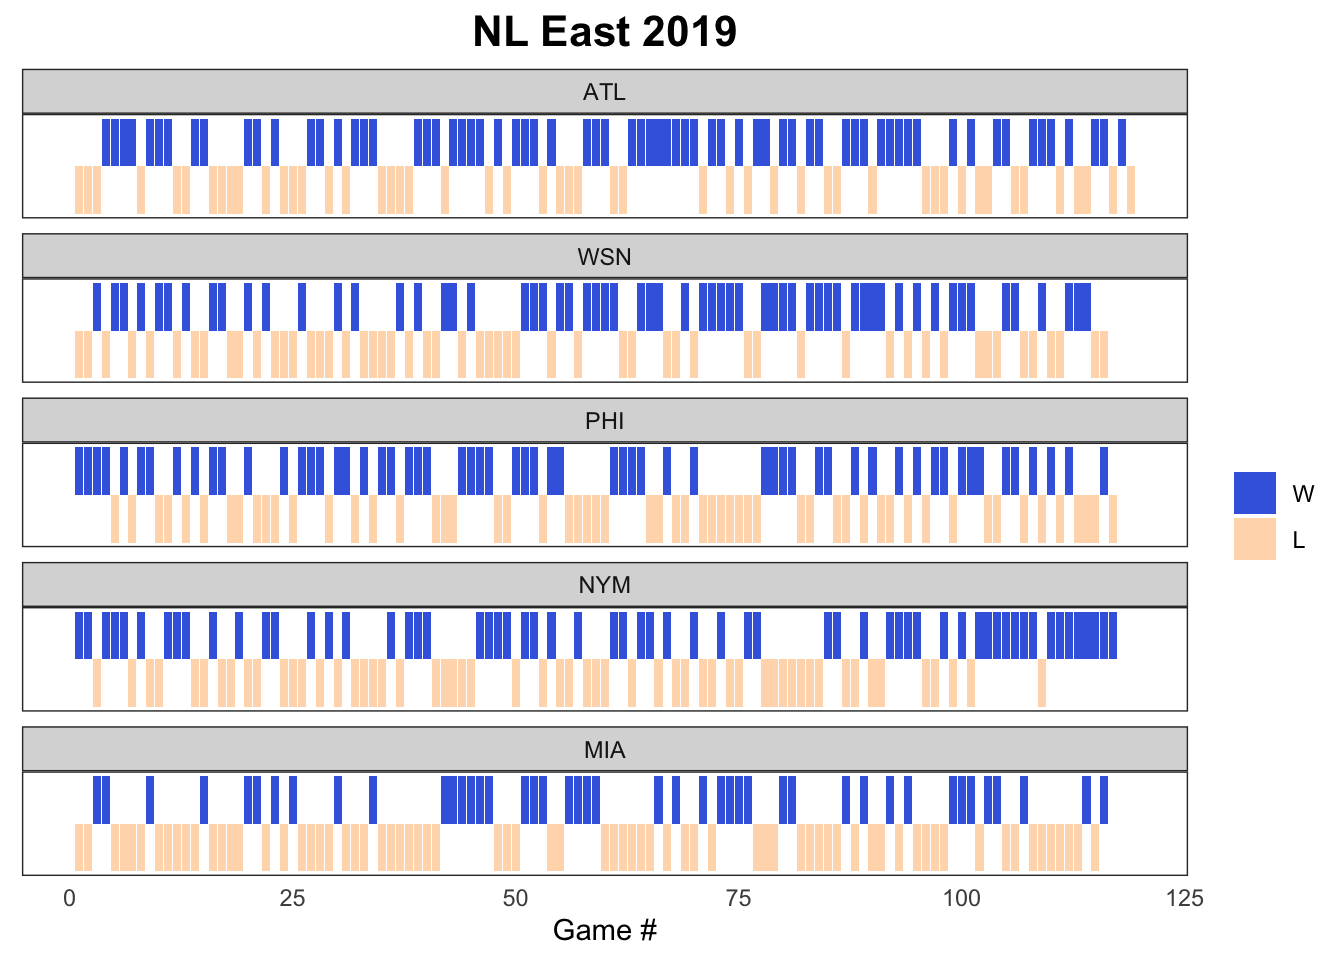
\includegraphics{gggallery_files/figure-latex/unnamed-chunk-107-1.pdf}

\hypertarget{nleastgamesabove}{%
\chapter*{NL East Teams Games above .500 in 2019}\label{nleastgamesabove}}
\addcontentsline{toc}{chapter}{NL East Teams Games above .500 in 2019}

\hypertarget{nleastgamesabovedata}{%
\subsubsection*{Data}\label{nleastgamesabovedata}}
\addcontentsline{toc}{subsubsection}{Data}

\begin{Shaded}
\begin{Highlighting}[]
\NormalTok{nleast <-}\StringTok{ }\KeywordTok{bind_rows}\NormalTok{(atl, phi, was, nym, mia)}
\end{Highlighting}
\end{Shaded}

\hypertarget{nleastgamesabovecode}{%
\subsubsection*{Code}\label{nleastgamesabovecode}}
\addcontentsline{toc}{subsubsection}{Code}

\begin{Shaded}
\begin{Highlighting}[]
\NormalTok{Month =}\StringTok{ }\KeywordTok{c}\NormalTok{(}\StringTok{"Jan"}\NormalTok{, }\StringTok{"Feb"}\NormalTok{, }\StringTok{"Mar"}\NormalTok{, }\StringTok{"Apr"}\NormalTok{, }\StringTok{"May"}\NormalTok{, }\StringTok{"Jun"}\NormalTok{, }\StringTok{"Jul"}\NormalTok{, }\StringTok{"Aug"}\NormalTok{, }\StringTok{"Sep"}\NormalTok{, }\StringTok{"Oct"}\NormalTok{, }\StringTok{"Nov"}\NormalTok{, }\StringTok{"Dec"}\NormalTok{)}

\NormalTok{month_num_table <-}\StringTok{ }\KeywordTok{data.frame}\NormalTok{(Month, }\DataTypeTok{MonthNum =} \DecValTok{1}\OperatorTok{:}\DecValTok{12}\NormalTok{)}

\NormalTok{nleast <-}\StringTok{ }\KeywordTok{separate}\NormalTok{(nleast, Date, }\DataTypeTok{into =} \KeywordTok{c}\NormalTok{(}\StringTok{"WeekDay"}\NormalTok{, }\StringTok{"Month"}\NormalTok{, }\StringTok{"Day"}\NormalTok{), }\DataTypeTok{sep =} \StringTok{" "}\NormalTok{) }\OperatorTok
\StringTok{  }\KeywordTok{mutate}\NormalTok{(}\DataTypeTok{Day =} \KeywordTok{as.integer}\NormalTok{(Day))}
\end{Highlighting}
\end{Shaded}

\begin{verbatim}
## Warning: Expected 3 pieces. Additional pieces discarded in 14 rows [19, 20,
## 191, 192, 308, 309, 336, 337, 418, 419, 464, 465, 579, 580].
\end{verbatim}

\begin{Shaded}
\begin{Highlighting}[]
\NormalTok{nleast <-}\StringTok{ }\KeywordTok{left_join}\NormalTok{(nleast, month_num_table, }\DataTypeTok{by =} \StringTok{"Month"}\NormalTok{) }\OperatorTok
\StringTok{  }\KeywordTok{mutate}\NormalTok{(}\DataTypeTok{MonthNum =} \KeywordTok{sprintf}\NormalTok{(}\StringTok{"%02d"}\NormalTok{, }\KeywordTok{as.numeric}\NormalTok{(MonthNum)),}
         \DataTypeTok{Day =} \KeywordTok{sprintf}\NormalTok{(}\StringTok{"%02d"}\NormalTok{, }\KeywordTok{as.numeric}\NormalTok{(Day)),}
         \DataTypeTok{MonthDay =} \KeywordTok{paste}\NormalTok{(MonthNum, Day, }\DataTypeTok{sep =} \StringTok{"-"}\NormalTok{)) }\OperatorTok
\StringTok{  }\KeywordTok{arrange}\NormalTok{(MonthDay)}
\end{Highlighting}
\end{Shaded}

\begin{verbatim}
## Warning: Column `Month` joining character vector and factor, coercing into
## character vector
\end{verbatim}

\begin{Shaded}
\begin{Highlighting}[]
\NormalTok{nleast}\OperatorTok{$}\NormalTok{MonthDay <-}\StringTok{ }\KeywordTok{factor}\NormalTok{(nleast}\OperatorTok{$}\NormalTok{MonthDay)}
\NormalTok{games_}\DecValTok{500}\NormalTok{_plot <-}\StringTok{ }\KeywordTok{ggplot}\NormalTok{(}\DataTypeTok{data =}\NormalTok{ nleast, }\KeywordTok{aes}\NormalTok{(}\DataTypeTok{x =}\NormalTok{ MonthDay, }\DataTypeTok{y =}\NormalTok{ games_updown, }\DataTypeTok{group =}\NormalTok{ Tm, }\DataTypeTok{colour =}\NormalTok{ Tm)) }\OperatorTok{+}
\StringTok{  }\KeywordTok{geom_step}\NormalTok{() }\OperatorTok{+}
\StringTok{  }\KeywordTok{theme_bw}\NormalTok{() }\OperatorTok{+}
\StringTok{  }\KeywordTok{geom_vline}\NormalTok{(}\DataTypeTok{xintercept =} \DecValTok{5}\NormalTok{, }\DataTypeTok{linetype =} \StringTok{"dashed"}\NormalTok{, }\DataTypeTok{colour =} \StringTok{"grey"}\NormalTok{) }\OperatorTok{+}
\StringTok{  }\KeywordTok{geom_vline}\NormalTok{(}\DataTypeTok{xintercept =} \DecValTok{35}\NormalTok{, }\DataTypeTok{linetype =} \StringTok{"dashed"}\NormalTok{, }\DataTypeTok{colour =} \StringTok{"grey"}\NormalTok{) }\OperatorTok{+}
\StringTok{  }\KeywordTok{geom_vline}\NormalTok{(}\DataTypeTok{xintercept =} \DecValTok{66}\NormalTok{, }\DataTypeTok{linetype =} \StringTok{"dashed"}\NormalTok{, }\DataTypeTok{colour =} \StringTok{"grey"}\NormalTok{) }\OperatorTok{+}
\StringTok{  }\KeywordTok{geom_vline}\NormalTok{(}\DataTypeTok{xintercept =} \DecValTok{96}\NormalTok{, }\DataTypeTok{linetype =} \StringTok{"dashed"}\NormalTok{, }\DataTypeTok{colour =} \StringTok{"grey"}\NormalTok{) }\OperatorTok{+}
\StringTok{  }\KeywordTok{geom_vline}\NormalTok{(}\DataTypeTok{xintercept =} \DecValTok{122}\NormalTok{, }\DataTypeTok{linetype =} \StringTok{"dashed"}\NormalTok{, }\DataTypeTok{colour =} \StringTok{"grey"}\NormalTok{) }\OperatorTok{+}
\StringTok{  }\KeywordTok{geom_text}\NormalTok{(}\KeywordTok{aes}\NormalTok{(}\DecValTok{10}\NormalTok{,}\DecValTok{22}\NormalTok{,}\DataTypeTok{label =} \StringTok{"April"}\NormalTok{), }\DataTypeTok{colour =} \StringTok{"grey"}\NormalTok{) }\OperatorTok{+}
\StringTok{  }\KeywordTok{geom_text}\NormalTok{(}\KeywordTok{aes}\NormalTok{(}\DecValTok{40}\NormalTok{,}\DecValTok{22}\NormalTok{,}\DataTypeTok{label =} \StringTok{"May"}\NormalTok{), }\DataTypeTok{colour =} \StringTok{"grey"}\NormalTok{) }\OperatorTok{+}
\StringTok{  }\KeywordTok{geom_text}\NormalTok{(}\KeywordTok{aes}\NormalTok{(}\DecValTok{71}\NormalTok{,}\DecValTok{22}\NormalTok{,}\DataTypeTok{label =} \StringTok{"June"}\NormalTok{), }\DataTypeTok{colour =} \StringTok{"grey"}\NormalTok{) }\OperatorTok{+}
\StringTok{  }\KeywordTok{geom_text}\NormalTok{(}\KeywordTok{aes}\NormalTok{(}\DecValTok{101}\NormalTok{,}\DecValTok{22}\NormalTok{,}\DataTypeTok{label =} \StringTok{"July"}\NormalTok{), }\DataTypeTok{colour =} \StringTok{"grey"}\NormalTok{) }\OperatorTok{+}
\StringTok{  }\KeywordTok{ylab}\NormalTok{(}\StringTok{"Games above .500"}\NormalTok{) }\OperatorTok{+}
\StringTok{  }\KeywordTok{ggtitle}\NormalTok{(}\StringTok{"NL East 2019"}\NormalTok{) }\OperatorTok{+}
\StringTok{  }\KeywordTok{theme}\NormalTok{(}\DataTypeTok{axis.title.x=}\KeywordTok{element_blank}\NormalTok{(),}
        \DataTypeTok{axis.ticks.x =} \KeywordTok{element_blank}\NormalTok{(),}
        \DataTypeTok{axis.text.x =} \KeywordTok{element_blank}\NormalTok{(),}
        \DataTypeTok{axis.ticks.y =} \KeywordTok{element_blank}\NormalTok{(),}
        \DataTypeTok{panel.grid.major.x =} \KeywordTok{element_blank}\NormalTok{(),}
        \DataTypeTok{panel.grid.minor.x =} \KeywordTok{element_blank}\NormalTok{(),}
        \DataTypeTok{legend.title =} \KeywordTok{element_blank}\NormalTok{(),}
        \DataTypeTok{plot.title =} \KeywordTok{element_text}\NormalTok{(}\DataTypeTok{size =} \DecValTok{16}\NormalTok{, }\DataTypeTok{face =} \StringTok{"bold"}\NormalTok{, }\DataTypeTok{hjust =} \FloatTok{0.5}\NormalTok{))}


\NormalTok{games_}\DecValTok{500}\NormalTok{_plot}
\end{Highlighting}
\end{Shaded}

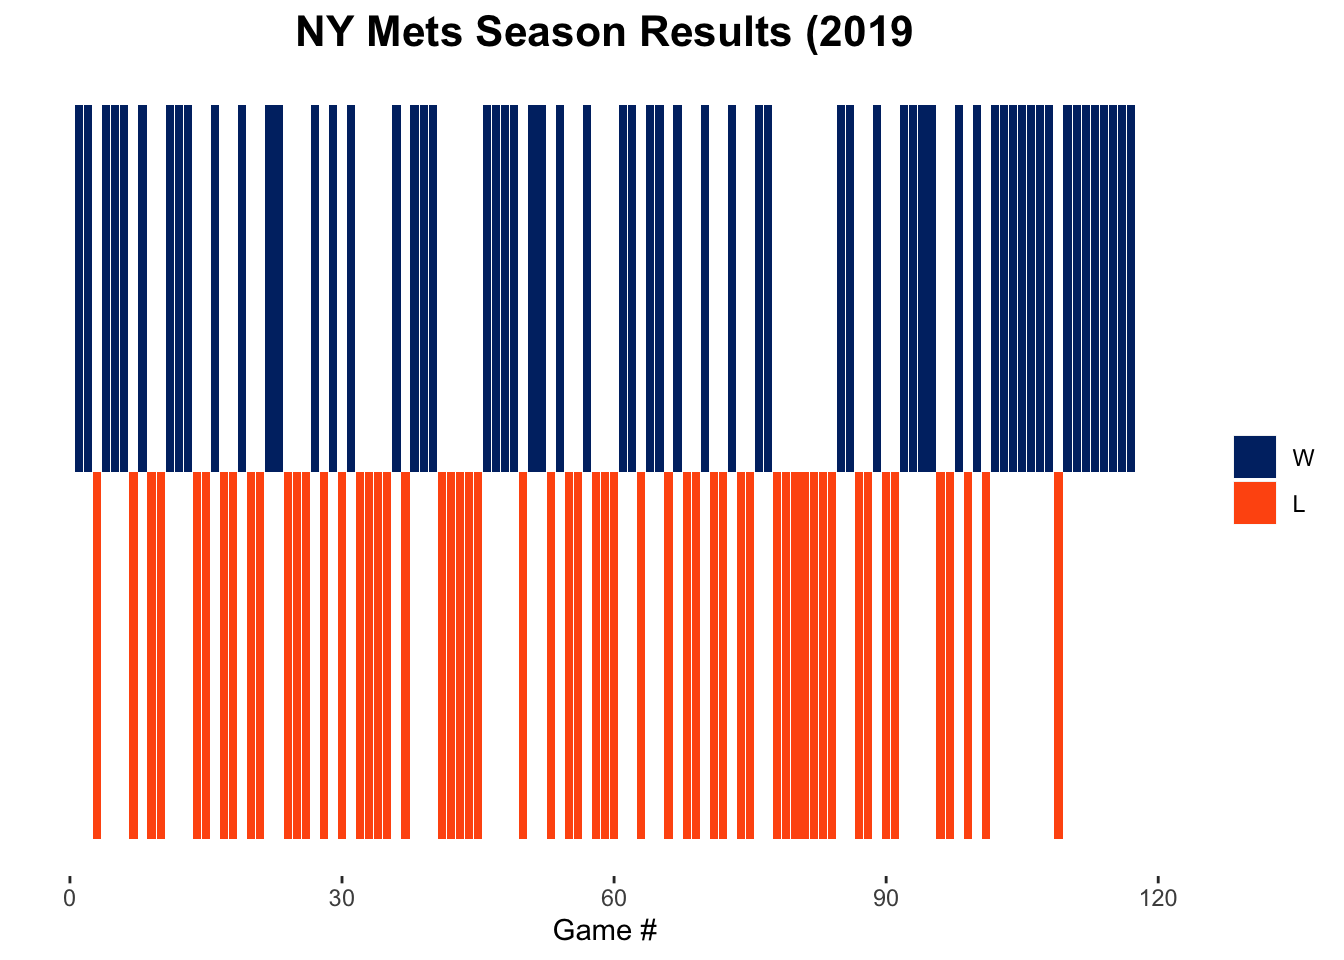
\includegraphics{gggallery_files/figure-latex/unnamed-chunk-111-1.pdf}

\hypertarget{chihist}{%
\chapter*{Chicago Employee Salaries}\label{chihist}}
\addcontentsline{toc}{chapter}{Chicago Employee Salaries}

\hypertarget{chihistdata}{%
\subsubsection*{Data}\label{chihistdata}}
\addcontentsline{toc}{subsubsection}{Data}

This plot uses the \emph{chi\_emps} data frame of the \emph{gcubed} package.

\begin{Shaded}
\begin{Highlighting}[]
\NormalTok{df <-}\StringTok{ }\KeywordTok{filter}\NormalTok{(chi_emps, SalHour }\OperatorTok{==}\StringTok{ "Salary"}\NormalTok{)}
\end{Highlighting}
\end{Shaded}

\hypertarget{chihistcode}{%
\subsubsection*{Code for plot}\label{chihistcode}}
\addcontentsline{toc}{subsubsection}{Code for plot}

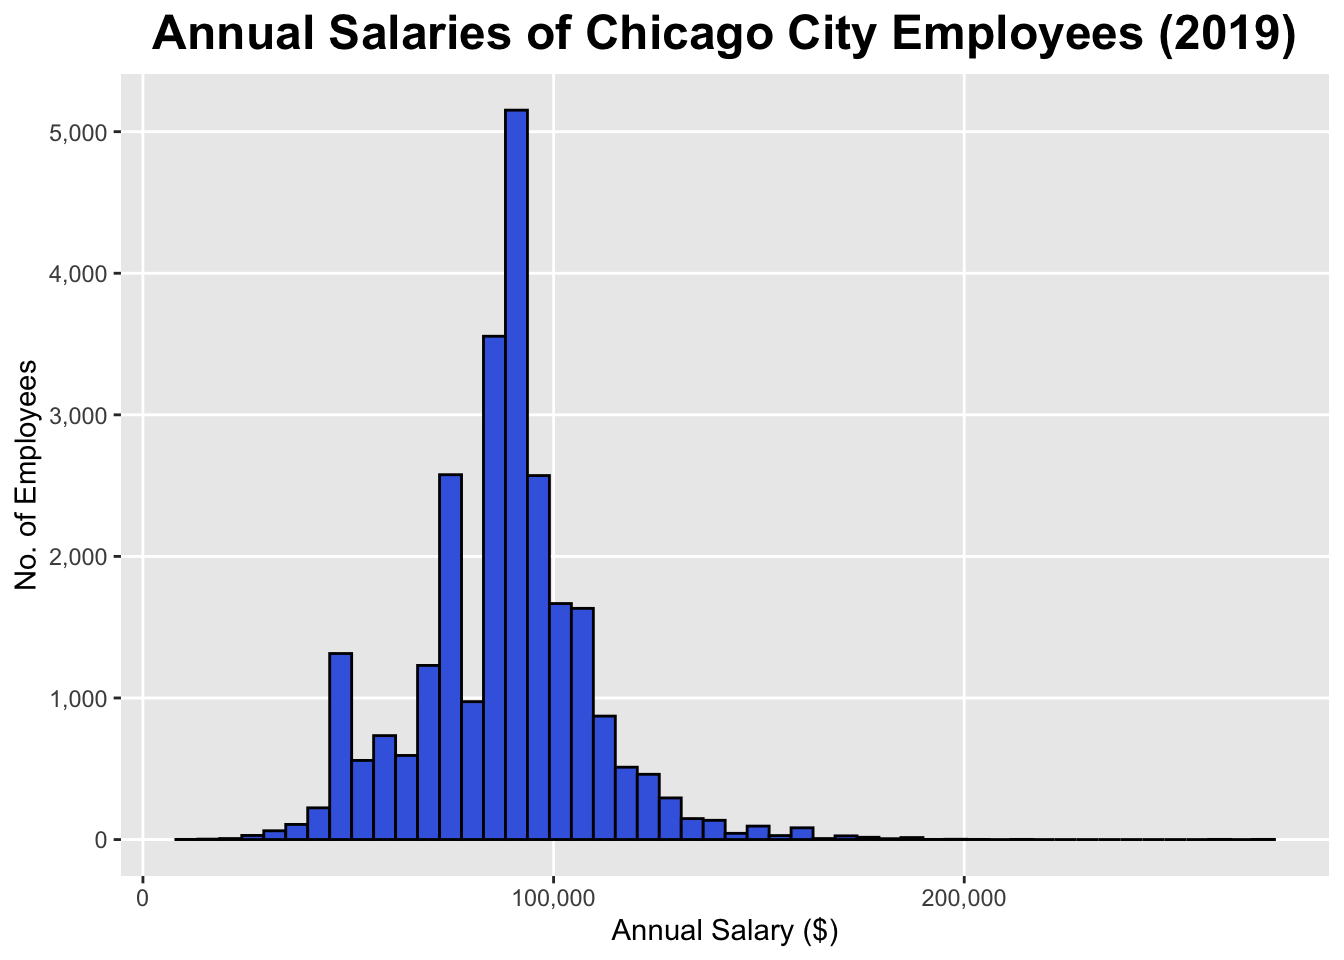
\includegraphics{gggallery_files/figure-latex/unnamed-chunk-115-1.pdf}

\begin{Shaded}
\begin{Highlighting}[]
\KeywordTok{ggsave}\NormalTok{(}\StringTok{"images/ChicagoEmployeeSalariesHist.png"}\NormalTok{, chi_emps_hist, }\DataTypeTok{width =} \DecValTok{7}\NormalTok{, }\DataTypeTok{height =} \DecValTok{7}\NormalTok{)}
\end{Highlighting}
\end{Shaded}

\hypertarget{comphists}{%
\chapter*{Chicago Histograms Faceted}\label{comphists}}
\addcontentsline{toc}{chapter}{Chicago Histograms Faceted}

\hypertarget{comphistsdata}{%
\subsubsection*{Data}\label{comphistsdata}}
\addcontentsline{toc}{subsubsection}{Data}

This plot uses the \emph{chi\_emps} data frame from package \emph{gcubed}.

First, find the 3 departments with the most salaried employees.

\begin{Shaded}
\begin{Highlighting}[]
\NormalTok{df <-}\StringTok{ }\KeywordTok{filter}\NormalTok{(chi_emps, SalHour }\OperatorTok{==}\StringTok{ "Salary"}\NormalTok{) }
\NormalTok{large_dept_names <-}\StringTok{ }\KeywordTok{names}\NormalTok{(}\KeywordTok{sort}\NormalTok{(}\KeywordTok{table}\NormalTok{(df}\OperatorTok{$}\NormalTok{Department), }\DataTypeTok{decreasing =} \OtherTok{TRUE}\NormalTok{))[}\DecValTok{1}\OperatorTok{:}\DecValTok{3}\NormalTok{]}
\NormalTok{large_dept_names}
\end{Highlighting}
\end{Shaded}

\begin{verbatim}
## [1] "POLICE" "FIRE"   "OEMC"
\end{verbatim}

\begin{Shaded}
\begin{Highlighting}[]
\NormalTok{large_depts <-}\StringTok{ }\NormalTok{chicago_salaries[chicago_salaries}\OperatorTok{$}\NormalTok{Department }\OperatorTok\StringTok{ }\NormalTok{large_dept_names, ]}
\KeywordTok{head}\NormalTok{(large_depts)}
\end{Highlighting}
\end{Shaded}

\begin{verbatim}
## # A tibble: 6 x 4
##   Name               Titles                         Department AnnualSalary
##   <chr>              <chr>                          <chr>             <dbl>
## 1 AARON,  JEFFERY M  SERGEANT                       POLICE           101442
## 2 AARON,  KARINA     POLICE OFFICER (ASSIGNED AS D~ POLICE            94122
## 3 ABARCA,  FRANCES J POLICE OFFICER                 POLICE            48078
## 4 ABBATEMARCO,  JAM~ FIRE ENGINEER-EMT              FIRE             103350
## 5 ABBATE,  TERRY M   POLICE OFFICER                 POLICE            93354
## 6 ABBOTT,  CARMELLA  POLICE OFFICER                 POLICE            68616
\end{verbatim}

\hypertarget{comphistscode}{%
\subsubsection*{Code for plot}\label{comphistscode}}
\addcontentsline{toc}{subsubsection}{Code for plot}

\begin{Shaded}
\begin{Highlighting}[]
\NormalTok{chi_comp_plt <-}\StringTok{ }\KeywordTok{ggplot}\NormalTok{(large_depts, }\KeywordTok{aes}\NormalTok{(}\DataTypeTok{x =}\NormalTok{ AnnualSalary, }\DataTypeTok{fill =}\NormalTok{ Department)) }\OperatorTok{+}\StringTok{ }
\StringTok{         }\KeywordTok{geom_histogram}\NormalTok{(}\DataTypeTok{bins =} \DecValTok{50}\NormalTok{, }\DataTypeTok{colour =} \StringTok{"black"}\NormalTok{) }\OperatorTok{+}\StringTok{ }
\StringTok{         }\KeywordTok{facet_wrap}\NormalTok{(}\OperatorTok{~}\NormalTok{Department, }\DataTypeTok{ncol =} \DecValTok{1}\NormalTok{, }\DataTypeTok{scales =} \StringTok{"free_y"}\NormalTok{) }\OperatorTok{+}\StringTok{ }
\StringTok{  }\KeywordTok{theme_bw}\NormalTok{() }\OperatorTok{+}\StringTok{ }
\StringTok{  }\KeywordTok{scale_x_continuous}\NormalTok{(}\DataTypeTok{label =}\NormalTok{ comma) }\OperatorTok{+}\StringTok{ }
\StringTok{  }\KeywordTok{scale_y_continuous}\NormalTok{(}\DataTypeTok{label =}\NormalTok{ comma) }\OperatorTok{+}\StringTok{ }
\StringTok{  }\KeywordTok{xlab}\NormalTok{(}\StringTok{"Annual Salary ($)"}\NormalTok{) }\OperatorTok{+}\StringTok{ }\KeywordTok{ylab}\NormalTok{(}\StringTok{"# of Employees"}\NormalTok{) }\OperatorTok{+}\StringTok{ }
\StringTok{  }\KeywordTok{ggtitle}\NormalTok{(}\StringTok{"Annual Salaries of Chicago City Employees (2019)"}\NormalTok{) }\OperatorTok{+}\StringTok{ }
\StringTok{  }\KeywordTok{theme}\NormalTok{(}\DataTypeTok{legend.position =} \StringTok{"none"}\NormalTok{, }\DataTypeTok{plot.title =} \KeywordTok{element_text}\NormalTok{(}\DataTypeTok{size =} \DecValTok{16}\NormalTok{, }\DataTypeTok{face =} \StringTok{"bold"}\NormalTok{, }\DataTypeTok{hjust =} \FloatTok{0.5}\NormalTok{))}

\NormalTok{chi_comp_plt}
\end{Highlighting}
\end{Shaded}

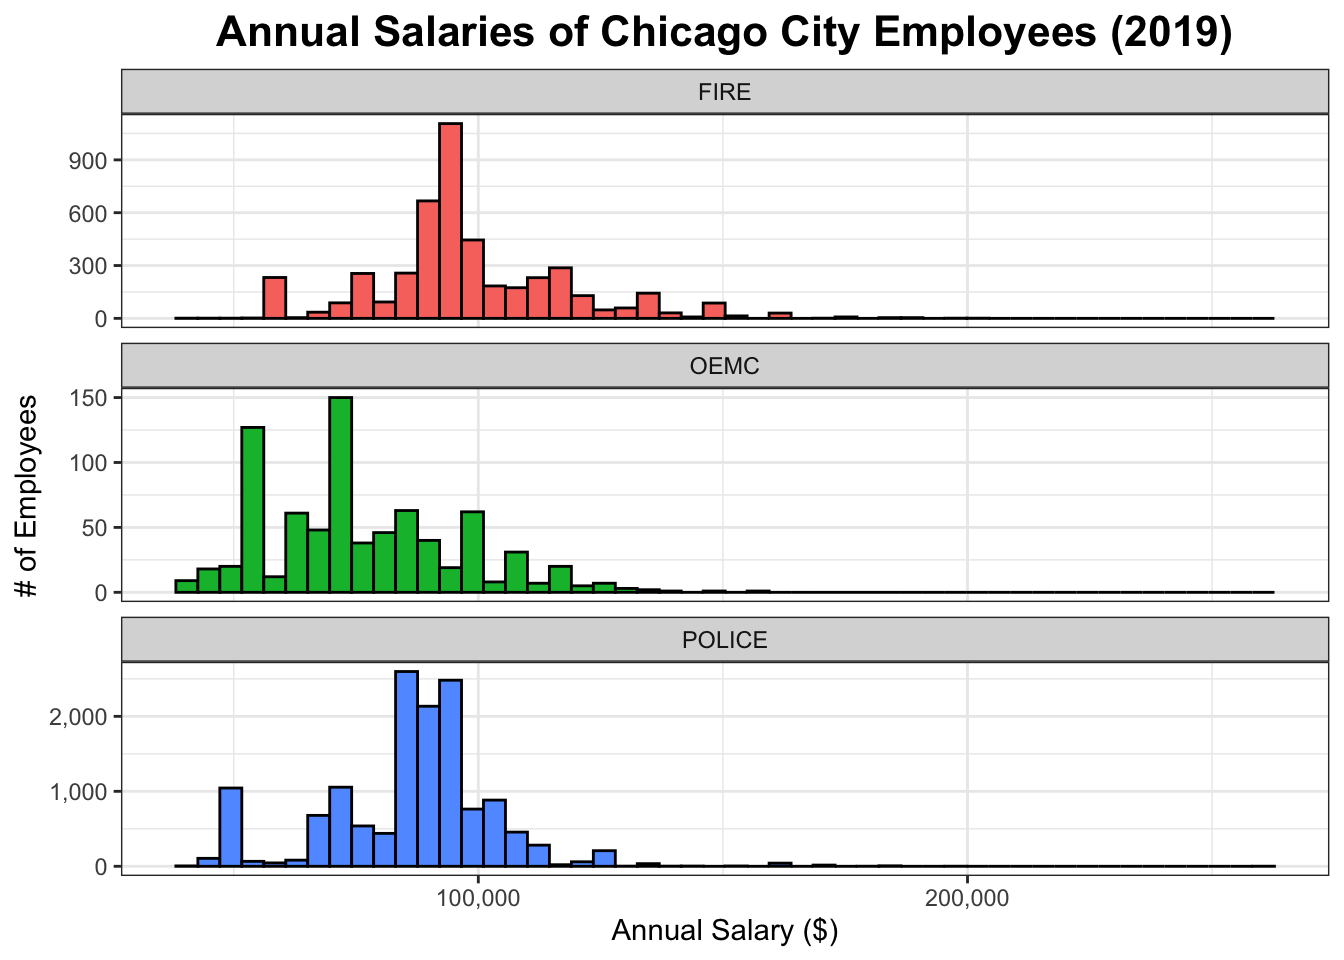
\includegraphics{gggallery_files/figure-latex/unnamed-chunk-119-1.pdf}

\hypertarget{nhanes}{%
\chapter*{Histogram of NHANES}\label{nhanes}}
\addcontentsline{toc}{chapter}{Histogram of NHANES}

\begin{Shaded}
\begin{Highlighting}[]
\KeywordTok{library}\NormalTok{(NHANES)}

\NormalTok{NHANES_adults <-}\StringTok{ }\KeywordTok{filter}\NormalTok{(NHANES, Age }\OperatorTok{>=}\StringTok{ }\DecValTok{18}\NormalTok{) }
\NormalTok{NHANES_bg <-}\StringTok{ }\KeywordTok{select}\NormalTok{(NHANES_adults, }\OperatorTok{-}\NormalTok{Gender) }


\NormalTok{nhanes_height_plot <-}\StringTok{ }\KeywordTok{ggplot}\NormalTok{(}\DataTypeTok{data =}\NormalTok{ NHANES_adults, }\KeywordTok{aes}\NormalTok{(}\DataTypeTok{x =}\NormalTok{ Height)) }\OperatorTok{+}
\StringTok{  }\KeywordTok{geom_histogram}\NormalTok{(}\DataTypeTok{data =}\NormalTok{ NHANES_bg, }\DataTypeTok{fill =} \StringTok{"grey"}\NormalTok{, }\DataTypeTok{alpha =} \FloatTok{.4}\NormalTok{) }\OperatorTok{+}
\StringTok{  }\KeywordTok{geom_histogram}\NormalTok{(}\DataTypeTok{mapping =} \KeywordTok{aes}\NormalTok{(}\DataTypeTok{fill =}\NormalTok{ Gender), }\DataTypeTok{colour =} \StringTok{"black"}\NormalTok{) }\OperatorTok{+}
\StringTok{  }\KeywordTok{facet_wrap}\NormalTok{(}\OperatorTok{~}\StringTok{ }\NormalTok{Gender, }\DataTypeTok{ncol =} \DecValTok{1}\NormalTok{) }\OperatorTok{+}
\StringTok{  }\KeywordTok{guides}\NormalTok{(}\DataTypeTok{fill =} \OtherTok{FALSE}\NormalTok{) }\OperatorTok{+}\StringTok{  }\CommentTok{# to remove the legend}
\StringTok{  }\KeywordTok{theme_bw}\NormalTok{() }\OperatorTok{+}\StringTok{ }\KeywordTok{xlab}\NormalTok{(}\StringTok{"Height (cm)"}\NormalTok{) }\OperatorTok{+}\StringTok{ }\KeywordTok{ggtitle}\NormalTok{(}\StringTok{"Heights of Surveyed US Adults (2009 - 2012)"}\NormalTok{)  }\OperatorTok{+}\StringTok{ }
\StringTok{  }\KeywordTok{theme}\NormalTok{(}\DataTypeTok{panel.grid.minor =} \KeywordTok{element_blank}\NormalTok{(), }
        \DataTypeTok{plot.title =} \KeywordTok{element_text}\NormalTok{(}\DataTypeTok{size =} \DecValTok{18}\NormalTok{, }\DataTypeTok{face =} \StringTok{"bold"}\NormalTok{, }\DataTypeTok{hjust =} \FloatTok{0.5}\NormalTok{))}
  

\NormalTok{nhanes_height_plot}
\end{Highlighting}
\end{Shaded}

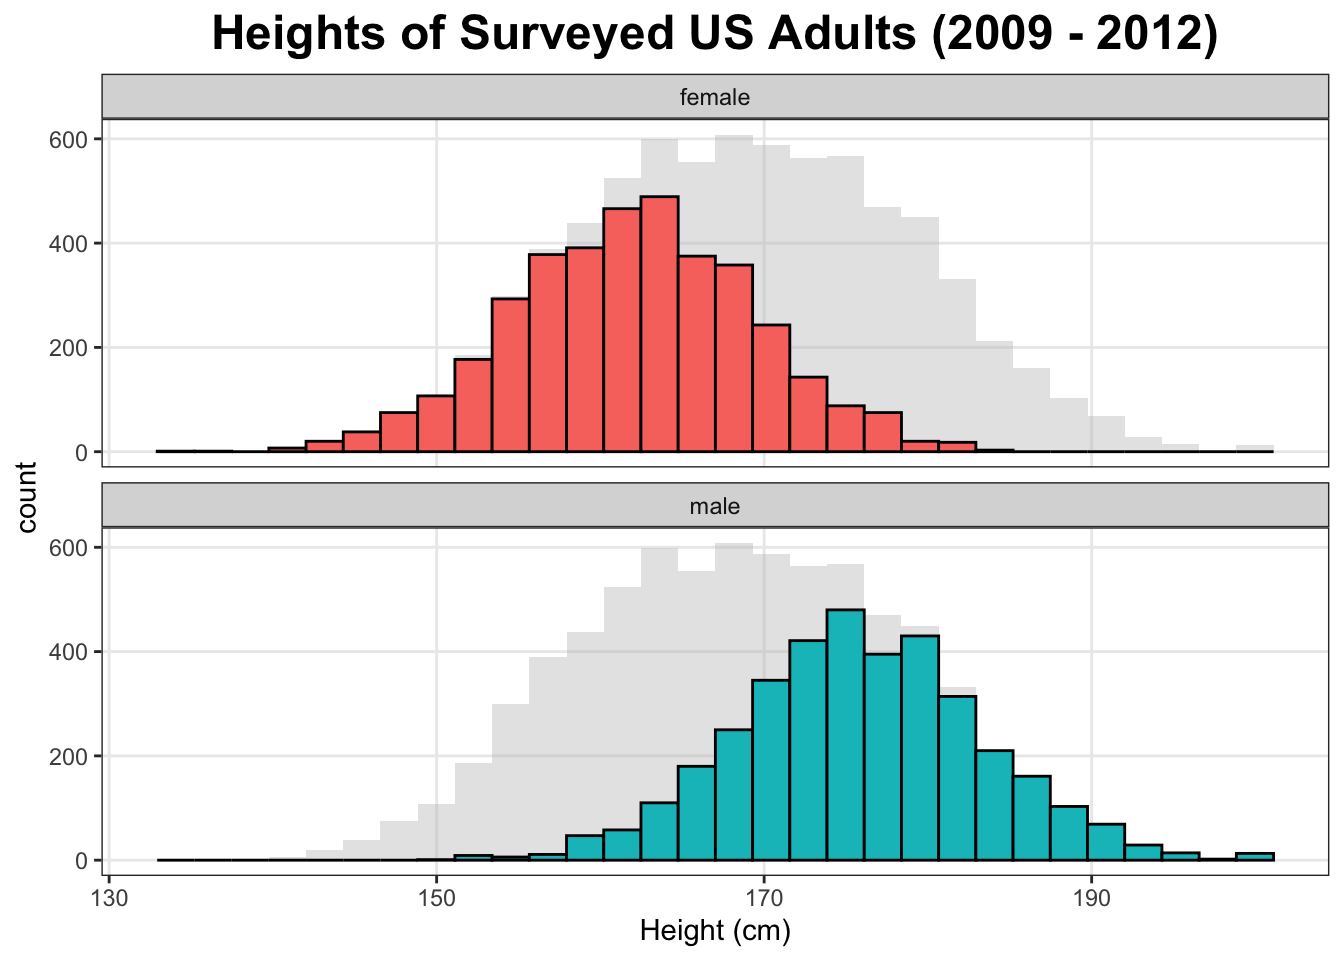
\includegraphics{gggallery_files/figure-latex/nhaneshists-1.pdf}

\begin{verbatim}
## Warning: Removed 114 rows containing non-finite values (stat_bin).
\end{verbatim}

\begin{verbatim}
## Warning: Removed 57 rows containing non-finite values (stat_bin).
\end{verbatim}

\hypertarget{chibox}{%
\chapter*{Chicago Employee Salary Box plot}\label{chibox}}
\addcontentsline{toc}{chapter}{Chicago Employee Salary Box plot}

\begin{Shaded}
\begin{Highlighting}[]
\NormalTok{dept_counts <-}\StringTok{ }\KeywordTok{table}\NormalTok{(chi_emps}\OperatorTok{$}\NormalTok{Department)}
\NormalTok{large_dept_counts <-}\StringTok{ }\NormalTok{dept_counts[dept_counts }\OperatorTok{>=}\StringTok{ }\DecValTok{500}\NormalTok{ ]}
\NormalTok{large_dept_names <-}\StringTok{ }\KeywordTok{names}\NormalTok{(large_dept_counts)}




\NormalTok{large_depts <-}\StringTok{ }\NormalTok{chi_emps[chi_emps}\OperatorTok{$}\NormalTok{Department }\OperatorTok\StringTok{ }\NormalTok{large_dept_names }\OperatorTok{&}\StringTok{ }\NormalTok{chi_emps}\OperatorTok{$}\NormalTok{SalHour }\OperatorTok{==}\StringTok{ "Salary"}\NormalTok{, ]}


\NormalTok{sorted_depts <-}\StringTok{ }\KeywordTok{group_by}\NormalTok{(large_depts, Department) }\OperatorTok\StringTok{ }
\StringTok{  }\KeywordTok{summarise}\NormalTok{(}\DataTypeTok{MedSal =} \KeywordTok{median}\NormalTok{(AnnualSalary)) }\OperatorTok\StringTok{ }
\StringTok{  }\KeywordTok{arrange}\NormalTok{(MedSal)}

\NormalTok{large_depts}\OperatorTok{$}\NormalTok{Department <-}\StringTok{ }\KeywordTok{factor}\NormalTok{(large_depts}\OperatorTok{$}\NormalTok{Department, }\DataTypeTok{levels =}\NormalTok{ sorted_depts}\OperatorTok{$}\NormalTok{Department) }


\NormalTok{chi_dept500_boxplot <-}\StringTok{ }\KeywordTok{ggplot}\NormalTok{(}\DataTypeTok{data =}\NormalTok{ large_depts, }\KeywordTok{aes}\NormalTok{(}\DataTypeTok{x =}\NormalTok{ Department, }\DataTypeTok{y =}\NormalTok{ AnnualSalary)) }\OperatorTok{+}\StringTok{ }
\StringTok{  }\KeywordTok{geom_boxplot}\NormalTok{() }\OperatorTok{+}\StringTok{ }
\StringTok{  }\KeywordTok{ggtitle}\NormalTok{(}\StringTok{"Salaries of Chicago City Govt Employees"}\NormalTok{) }\OperatorTok{+}\StringTok{ }
\StringTok{  }\KeywordTok{theme}\NormalTok{(}\DataTypeTok{plot.title =} \KeywordTok{element_text}\NormalTok{(}\DataTypeTok{size =} \DecValTok{16}\NormalTok{, }\DataTypeTok{face =} \StringTok{"bold"}\NormalTok{, }\DataTypeTok{hjust =} \FloatTok{0.5}\NormalTok{), }
        \DataTypeTok{axis.text.x =} \KeywordTok{element_text}\NormalTok{(}\DataTypeTok{angle =} \DecValTok{90}\NormalTok{),}
        \DataTypeTok{axis.title.x=}\KeywordTok{element_blank}\NormalTok{()) }\OperatorTok{+}\StringTok{ }
\StringTok{  }\KeywordTok{ylab}\NormalTok{(}\StringTok{"Annual Salary ($)"}\NormalTok{) }\OperatorTok{+}
\StringTok{  }\KeywordTok{scale_y_continuous}\NormalTok{(}\DataTypeTok{label =}\NormalTok{ comma)}

\NormalTok{chi_dept500_boxplot }
\end{Highlighting}
\end{Shaded}

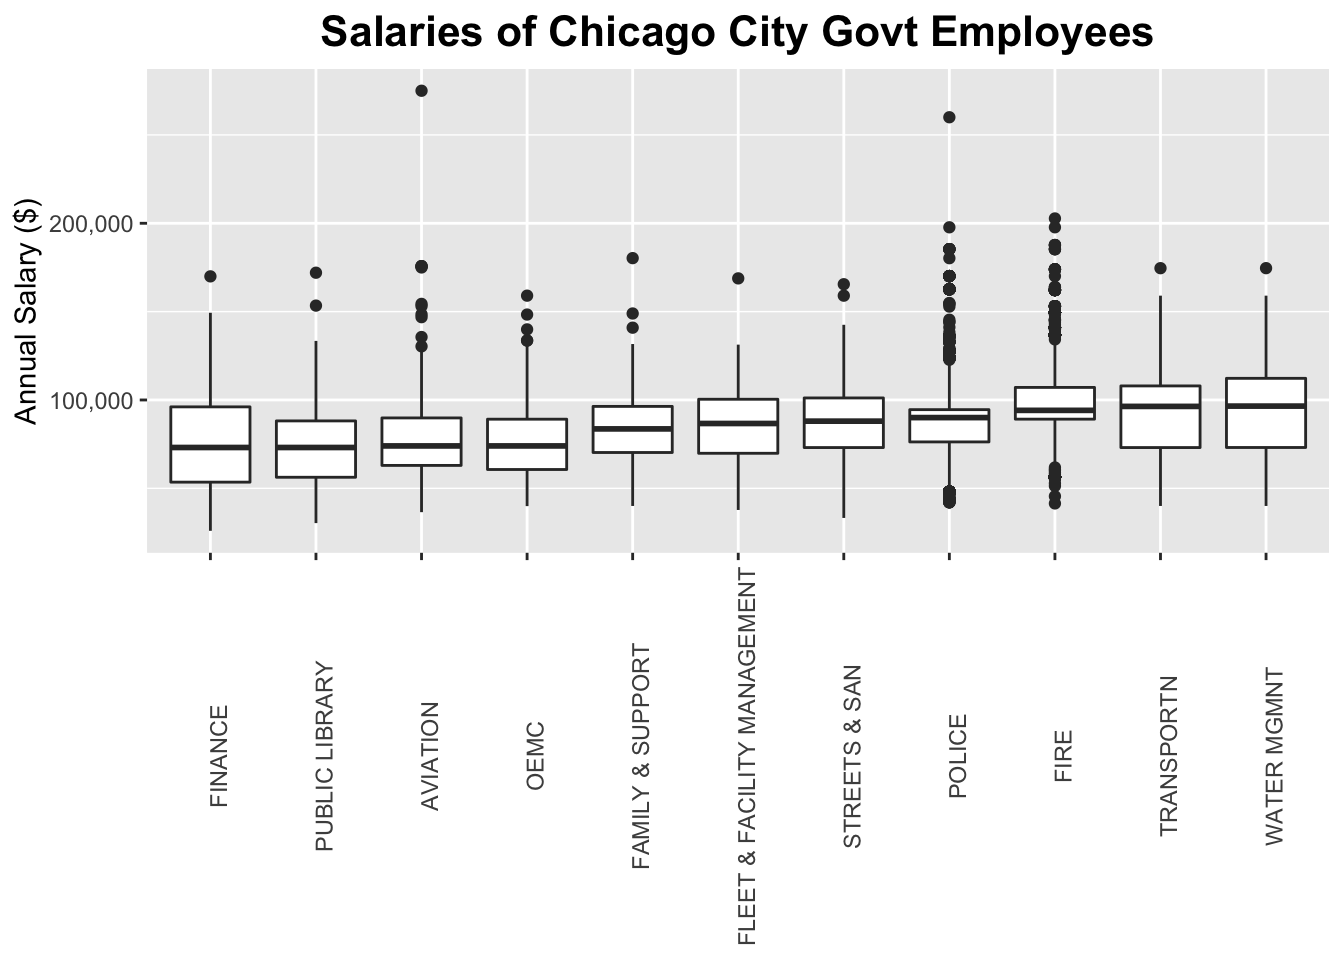
\includegraphics{gggallery_files/figure-latex/unnamed-chunk-122-1.pdf}

\hypertarget{chiridges}{%
\chapter*{Chicago City Salaries Compared: Density Ridges}\label{chiridges}}
\addcontentsline{toc}{chapter}{Chicago City Salaries Compared: Density Ridges}

\begin{Shaded}
\begin{Highlighting}[]
\NormalTok{df <-}\StringTok{ }\NormalTok{chicago_salaries}
\NormalTok{dept_counts <-}\StringTok{ }\KeywordTok{table}\NormalTok{(df}\OperatorTok{$}\NormalTok{Department)}
\NormalTok{large_dept_names <-}\StringTok{ }\KeywordTok{names}\NormalTok{(dept_counts[dept_counts }\OperatorTok{>}\StringTok{ }\DecValTok{500}\NormalTok{])}
\NormalTok{large_dept_names}
\end{Highlighting}
\end{Shaded}

\begin{verbatim}
## [1] "AVIATION"       "FINANCE"        "FIRE"           "OEMC"          
## [5] "POLICE"         "PUBLIC LIBRARY"
\end{verbatim}

\begin{Shaded}
\begin{Highlighting}[]
\NormalTok{df}\OperatorTok{$}\NormalTok{Dept <-}\StringTok{ }\KeywordTok{ifelse}\NormalTok{(df}\OperatorTok{$}\NormalTok{Department }\OperatorTok\StringTok{ }\NormalTok{large_dept_names, df}\OperatorTok{$}\NormalTok{Department, }\StringTok{"OTHER"}\NormalTok{)}
\KeywordTok{table}\NormalTok{(df}\OperatorTok{$}\NormalTok{Dept)}
\end{Highlighting}
\end{Shaded}

\begin{verbatim}
## 
##       AVIATION        FINANCE           FIRE           OEMC          OTHER 
##            583            534           4631            799           4432 
##         POLICE PUBLIC LIBRARY 
##          14060            702
\end{verbatim}

\begin{Shaded}
\begin{Highlighting}[]
\NormalTok{dept_levels <-}\StringTok{ }\KeywordTok{c}\NormalTok{(}\StringTok{"OTHER"}\NormalTok{, }\KeywordTok{rev}\NormalTok{(large_dept_names))}
\NormalTok{df}\OperatorTok{$}\NormalTok{Dept <-}\StringTok{ }\KeywordTok{factor}\NormalTok{(df}\OperatorTok{$}\NormalTok{Dept, }\DataTypeTok{levels =}\NormalTok{ dept_levels)}
\KeywordTok{library}\NormalTok{(ggridges)}
\NormalTok{chi_ridge_plt <-}\StringTok{ }\KeywordTok{ggplot}\NormalTok{(}\DataTypeTok{data =}\NormalTok{ df, }\KeywordTok{aes}\NormalTok{(}\DataTypeTok{x =}\NormalTok{ AnnualSalary, }\DataTypeTok{y =}\NormalTok{ Dept)) }\OperatorTok{+}\StringTok{ }
\StringTok{  }\KeywordTok{geom_density_ridges}\NormalTok{() }\OperatorTok{+}\StringTok{ }
\StringTok{  }\KeywordTok{scale_x_continuous}\NormalTok{(}\DataTypeTok{label=}\NormalTok{comma) }\OperatorTok{+}
\StringTok{  }\KeywordTok{ggtitle}\NormalTok{(}\StringTok{"Annual Salaries of Chicago City Employees (2019)"}\NormalTok{) }\OperatorTok{+}\StringTok{ }
\StringTok{  }\KeywordTok{theme}\NormalTok{(}\DataTypeTok{plot.title =} \KeywordTok{element_text}\NormalTok{(}\DataTypeTok{size =} \DecValTok{16}\NormalTok{, }\DataTypeTok{face =} \StringTok{"bold"}\NormalTok{, }\DataTypeTok{hjust =} \FloatTok{0.5}\NormalTok{))}

\NormalTok{chi_ridge_plt}
\end{Highlighting}
\end{Shaded}

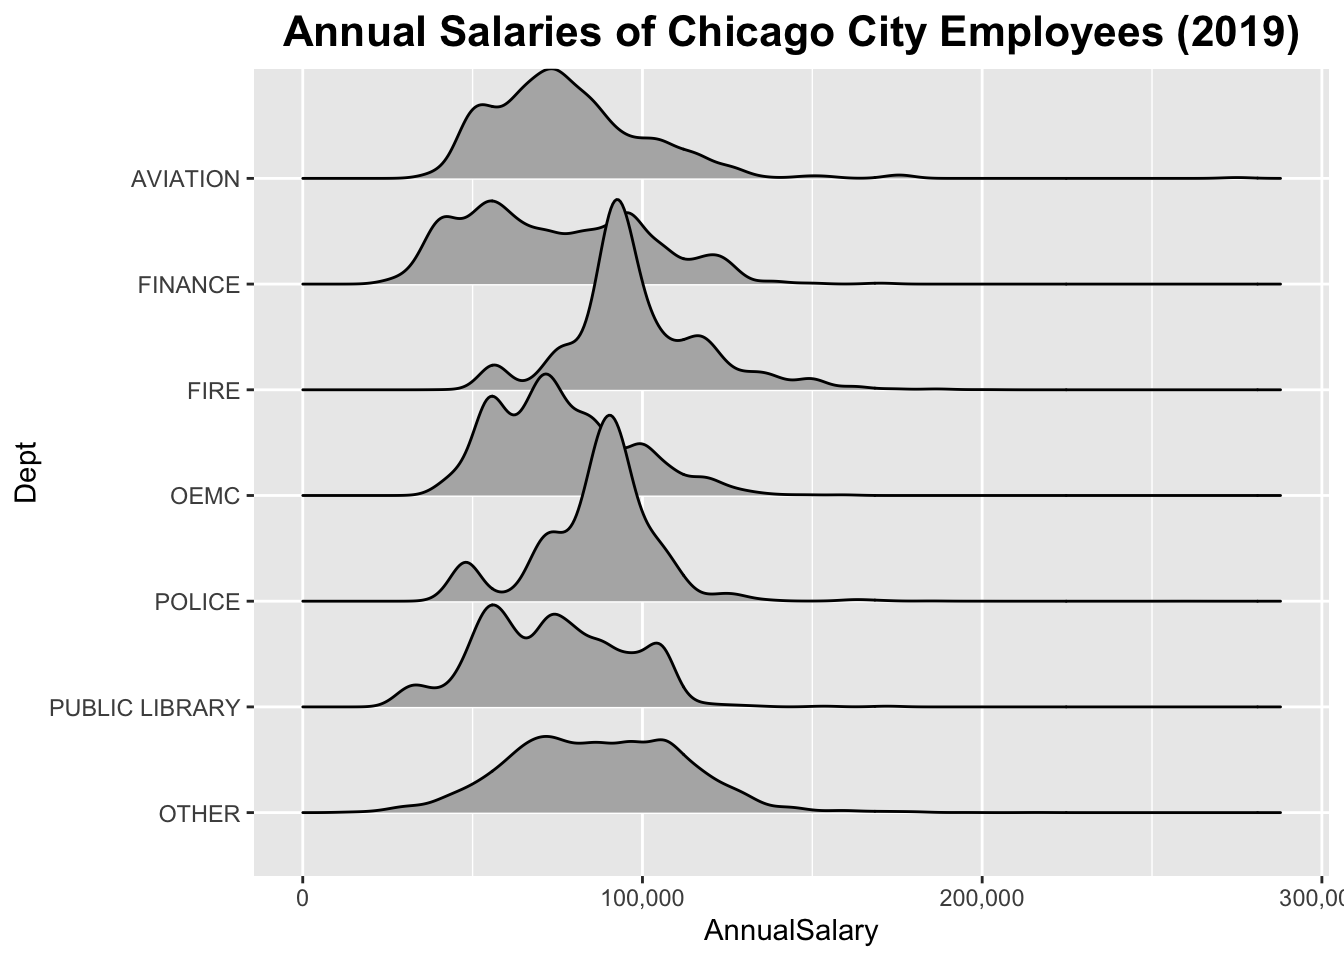
\includegraphics{gggallery_files/figure-latex/unnamed-chunk-126-1.pdf}

\bibliography{book.bib,packages.bib}


\end{document}
